%%%% Master thesis - LMS template (FAU Erlangen-Nuernberg)
%%%% Based on the LMS-Bericht-LaTeX template by Dipl.-Ing. Marcus Laumer
%%%% All files must be encoded in UTF-8.

\documentclass[
paper=A4,               % paper format
pagesize=auto,          % provide page size for compiler
fontsize=12pt,          % font size
DIV=16,                 % type area calculation
twoside=true,           % two-sided layout for printing
BCOR=20mm,              % binding correction for printing (ask at copy shop!)
parskip=false,          % space between paragraphs
chapterprefix=true,     % prefix before chapter names: Chapter #
listof=totoc,           % include lists of figures and tables in TOC
bibliography=totoc,     % include bibliography in TOC
headinclude=true,       % header included in type area
footinclude=false,      % footer included in type area
headsepline=true,       % separation line between header and text
footsepline=false,      % separation line between footer and text
headings=small,         % size of headings
numbers=noenddot        % no dot after chapter heading prefixes
] {scrbook}

\usepackage{lmodern}
\usepackage[T1]{fontenc}
\usepackage[utf8]{inputenc}
\usepackage[english]{babel}
\usepackage[onehalfspacing]{setspace}
\usepackage{amsmath,amssymb}
\usepackage{graphicx}
\usepackage{packages/wrapfig}
\usepackage[caption=false]{subfig}
\usepackage{array}
\usepackage{booktabs}
\usepackage{longtable}
\usepackage{placeins}
\usepackage{etoolbox}
\AtBeginEnvironment{longtable}{\singlespacing}
% Keep bibliography text at 12 pt while avoiding isolated entries on a new page.
\AtBeginEnvironment{thebibliography}{\singlespacing}
\usepackage{multirow}
% left-aligned fixed-width column: avoids heavy hyphenation in narrow columns
\newcolumntype{L}[1]{>{\raggedright\arraybackslash}p{#1}}
\usepackage{siunitx}
\usepackage{packages/xstring}
\usepackage{packages/suffix}
\usepackage[printonlyused]{packages/acronym}
\acrodef{LiDAR}{Light Detection and Ranging}
\acrodef{AP}{Average Precision}
\acrodef{MLP}{Multi-Layer Perceptron}
\acrodef{FPS}{Farthest Point Sampling}
\acrodef{MSG}{Multi-Scale Grouping}
\usepackage{pdfpages}
\usepackage[nocompress]{cite}
\usepackage[hidelinks]{hyperref}

\graphicspath{{figure/}}
\setkomafont{caption}{\normalfont\normalsize}
\setkomafont{captionlabel}{\normalfont\normalsize}
\newcommand{\thesisfigure}[4]{%
  \begin{figure}[!t]\centering
  \includegraphics[width=\linewidth]{#1.pdf}%
  \caption[#2]{#3}\label{#4}\end{figure}}
\raggedbottom
\widowpenalty=10000
\clubpenalty=10000
\emergencystretch=1.5em
\makeatletter
\let\tableinput\@@input
\renewcommand{\@pnumwidth}{2.5em}
\setlength{\@fptop}{0pt}
\makeatother

%%%% Float placement tuning.
%%%% The LaTeX defaults are conservative and push tables onto pages of their
%%%% own, leaving large holes in the preceding text page. These values allow a
%%%% float to share a page with more text and require a float page to be
%%%% better filled before it is created.
\setcounter{topnumber}{2}
\setcounter{bottomnumber}{1}
\setcounter{totalnumber}{3}
\renewcommand{\topfraction}{0.85}
\renewcommand{\bottomfraction}{0.65}
\renewcommand{\textfraction}{0.10}
\renewcommand{\floatpagefraction}{0.80}

\recalctypearea

\begin{document}

    \pagenumbering{Alph} % will not be displayed
    \begin{titlepage}
    \vspace*{6ex}
    \begin{center}
        \LARGE
        Friedrich-Alexander-Universität Erlangen-Nürnberg\\[1.5ex]
        \Large
        \textbf{Lehrstuhl für Multimediakommunikation und Signalverarbeitung}\\[1.5ex]
        Prof. Dr.-Ing. André Kaup\\
        \vfill
        \LARGE
        Master Thesis\\[3ex]
        \textbf{Investigating the Impact of\\Point Cloud Upsampling on\\3D Object Detection Performance}\\[3ex]
        Jiahui Shen\\
        \vfill
        \Large
        September 2026\\[1.5ex]
        \begin{tabular}{ll}
            Supervisor: & Marina Ritthaler, M.Sc.
        \end{tabular}
    \end{center}
\end{titlepage}

    \cleardoublepage
    % Signed thesis task / topic description. Replace topic/description.pdf
    % with the signed Masterthesis task sheet before submission.
    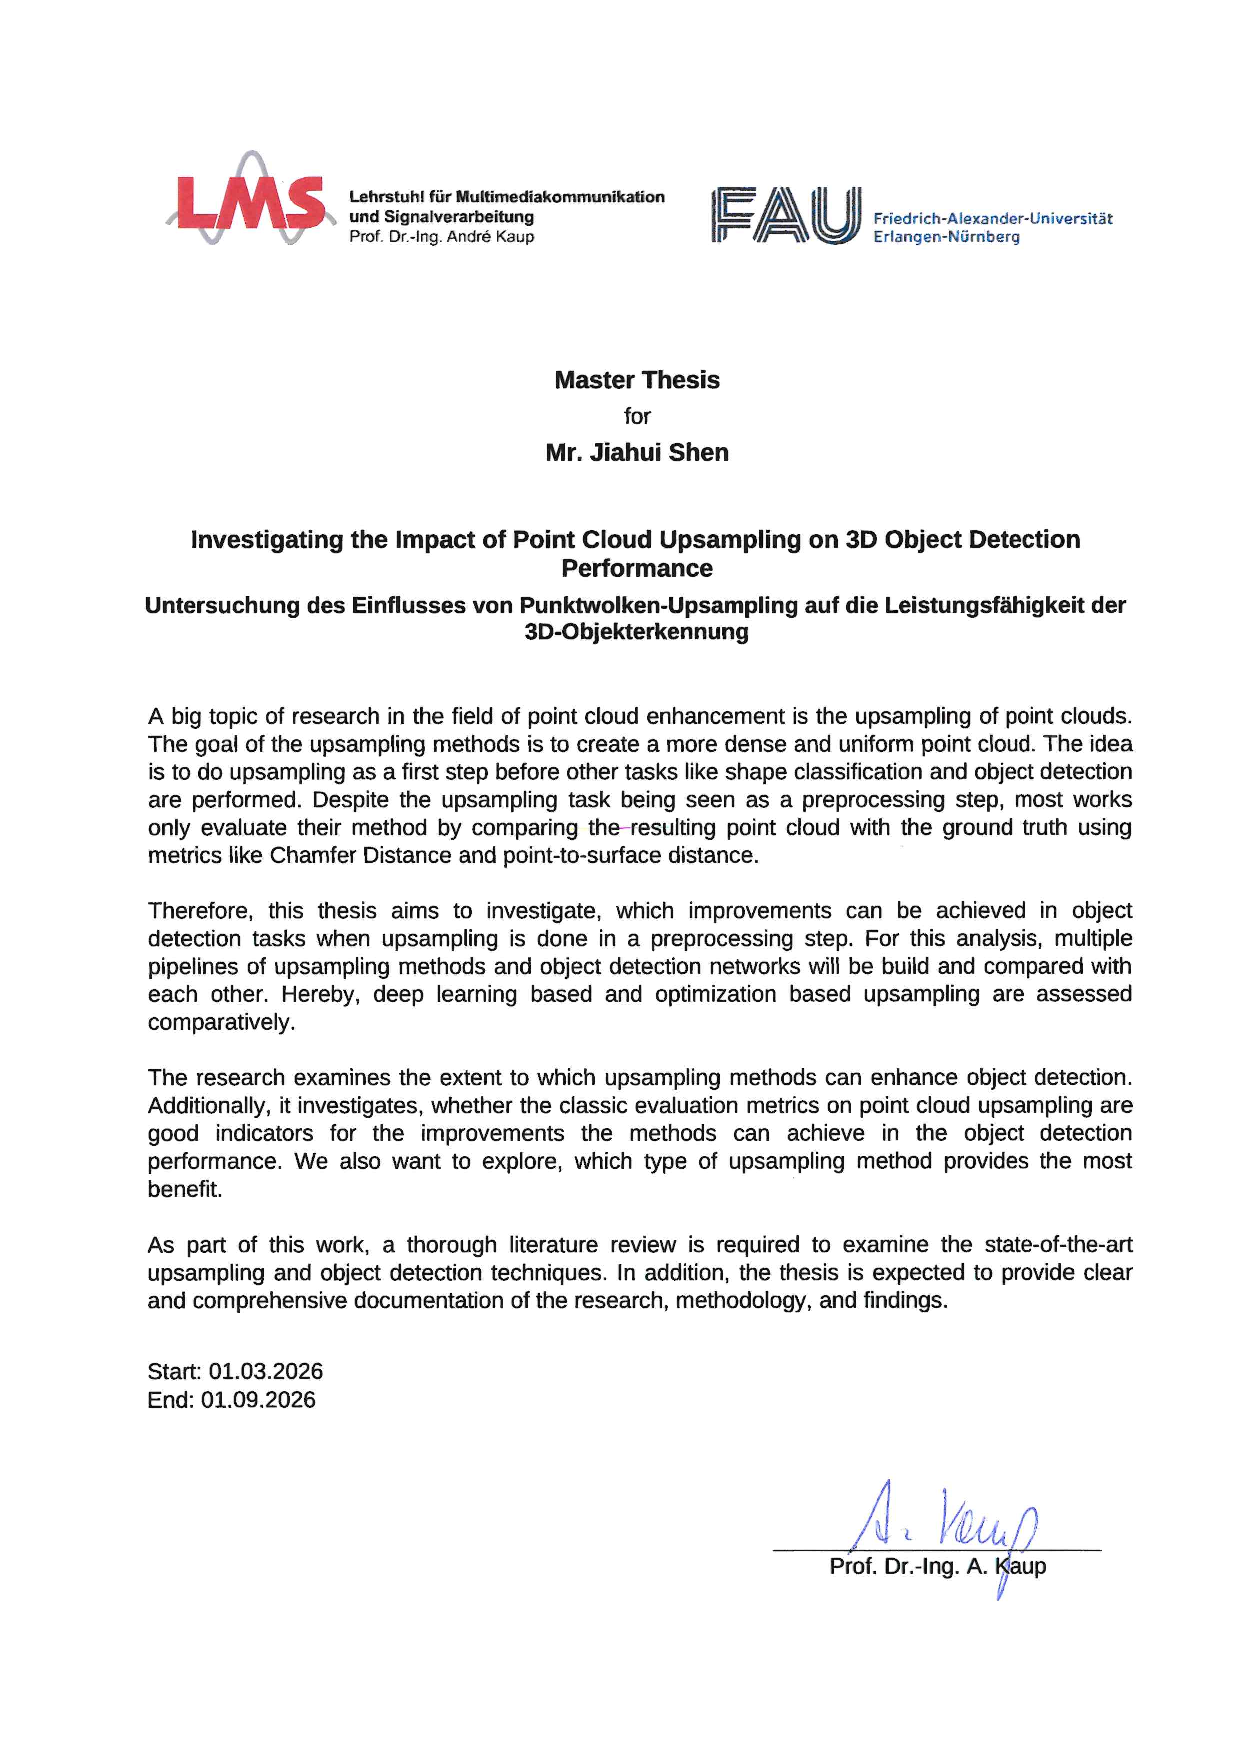
\includepdf[pages={1},scale={0.95}]{topic/description}
    \cleardoublepage

    \chapter*{Declaration}
\thispagestyle{empty}

\noindent
I confirm that I have written this thesis unaided and without using sources other than those listed and that this thesis has never been submitted to another examination authority and accepted as part of an examination achievement, neither in this form nor in a similar form.
All content that was taken from a third party either verbatim or in substance has been acknowledged as such.

\vspace{3cm}

\begin{minipage}[t]{0.45\textwidth}
    \rule{\textwidth}{0.5pt}\\
	Place, Date
\end{minipage}
\hfill
\begin{minipage}[t]{0.45\textwidth}
	\rule{\textwidth}{0.5pt}\\
	Jiahui Shen
\end{minipage}


    \frontmatter
    \pagenumbering{Roman}
    {\singlespacing\tableofcontents}
    \chapter*{Kurzfassung}\addcontentsline{toc}{chapter}{Kurzfassung}
Die Hochabtastung von Punktwolken erhöht die Anzahl räumlicher Abtastpunkte.
Ein Nutzen für nachgelagerte Wahrnehmungsaufgaben lässt sich jedoch nicht
allein aus geometrischen Abständen ableiten. Diese Arbeit untersucht die
Verdichtung einer ursprünglichen Eingabe sowie die Rekonstruktion nach
einer Reduktion auf ein Viertel der Punkte. Auf ModelNet40 werden EAR,
PDANS, PU-Net, PU-GCN und PU-EdgeFormer mit separat trainierten
PointNet++-Klassifikatoren und geometrischen Referenzen gleicher
Punktanzahl verglichen. Auf KITTI werden PointRCNN und CenterPoint
untersucht. Eine PU-GCN-Eingabe- und Detektoranpassungsstudie über drei
Epochen umfasst 20 Auswertungen. Anschließend wird das Training mit
Eingaben unter Erhalt der beobachteten Punkte verlängert. Jede
Hauptauswertung verwendet 3.769 Validierungsframes.

Bei der protokollierten, über Batches gemittelten Genauigkeit übertrifft
keine getestete Methode in ModelNet40-Linie~A die beste
Gesamtgenauigkeit der ursprünglichen Darstellung mit 1.024 Punkten
von 91,95\%. Nach der Ausdünnung verbessert PU-Net diese Genauigkeit
von 90,85\% auf 91,27\%, während PU-GCN in beiden Linien den niedrigsten
mittleren Chamfer-Abstand erreicht. Auf KITTI verschlechtern direkte
PU-GCN-Eingaben die Ergebnisse der unveränderten Detektoren. Der Erhalt
gemessener Punkte und die Anpassung der Detektoren verbessern die
Ergebnisse, übertreffen jedoch nicht die jeweiligen Referenzen. Das
verlängerte Training verbessert alle vier Detektor-Linien-Kombinationen
weiter und erfüllt das festgelegte Plateaukriterium für die
Car-Validierungsmetrik. Dennoch verbleiben Rückstände von 3,31 bis
11,28 AP-Punkten gegenüber den jeweiligen Linienreferenzen. Das
PU-GCN-Netz selbst verwendet weiterhin seine veröffentlichten Gewichte.

Diagnostische Versuche zu Patch-Normalisierung, Punktverarbeitung und
Voxelbelegung zeigen, warum gespeicherte Punktdichte und wirksame
Modelleingabe verschieden sind. Die Aussagekraft wird durch nur einen
Trainingsseed, die Auswahl des besten Klassifikators anhand des Testsatzes,
ungleiche Trainingsbudgets der Detektoren und die Auswahl ihrer
Checkpoints anhand desselben Validierungssatzes begrenzt. Geometrische Qualität allein reicht somit nicht aus, um einen Nutzen
für nachgelagerte Aufgaben nachzuweisen.

    \chapter*{Abstract}\addcontentsline{toc}{chapter}{Abstract}
Point-cloud upsampling increases the number of spatial samples, but its
benefit for downstream perception cannot be inferred from geometric
distance alone. This thesis evaluates densification of an original input
and recovery after fourfold sparsification on two complementary tasks.
The ModelNet40 study compares EAR, PDANS, PU-Net, PU-GCN, and PU-EdgeFormer
using separately trained PointNet++ classifiers and equal-cardinality
geometric references. The KITTI study evaluates point-based PointRCNN
and voxel-based CenterPoint, with a 20-arm PU-GCN input and three-epoch
detector-adaptation matrix, followed by extended observed-first training.
Each main evaluation covers 3,769 validation frames.

Using the recorded batch-aggregated accuracy, no tested method improves
ModelNet40 Line~A best overall accuracy over
the original 1,024-point representation at 91.95\%. After sparsification,
PU-Net raises best accuracy from 90.85\% to 91.27\%, while PU-GCN achieves
the lowest mean Chamfer distance in both lines. On KITTI, direct insertion
degrades frozen detection. Preserving measured points and adapting the
detectors recover performance but leave deficits relative to the
corresponding baselines. Extended adaptation further improves all four
detector--line conditions and meets the specified Car-validation plateau
criterion, but still leaves deficits of 3.31--11.28 AP points relative
to the line-specific references. PU-GCN itself retains its released
pretrained weights throughout this later study.

Patch-normalisation, point-reception, and voxel-occupancy diagnostics show
why stored density differs from effective task input. The findings are
bounded by single-seed classifier training, test-based best-checkpoint
selection, unequal detector-training budgets, and detector checkpoint
selection on the reported validation set. The combined evidence establishes a
limited object-level recovery benefit and partial scene-level recovery,
while showing that geometric fidelity alone is insufficient to establish
downstream utility.

    \chapter{Symbols and Notations}
Symbols are defined at their first use. The following list collects the
principal quantities; method-specific indices are defined locally.

\begin{singlespace}
\noindent\textbf{Point Sets and Scan Geometry}\par\nobreak\vspace{0.4em}
\noindent\begin{tabular}{@{}lL{0.71\linewidth}@{}}
$\mathcal P,\mathcal X$ & Input point sets\\
$\mathbf p_i,\mathbf x_i$ & Three-dimensional coordinates\\
$\iota_i$ & Reflectance associated with a measured point\\
$N_s,M_s$ & Original and sparse point counts in frame $s$\\
$\mathcal R$ & Geometric reference point set\\
\end{tabular}\par\vspace{0.8em}
\noindent\textbf{Networks and Detection}\par\nobreak\vspace{0.4em}
\noindent\begin{tabular}{@{}lL{0.71\linewidth}@{}}
$\phi_\theta,f_\theta$ & Learned feature map and classifier\\
$\mathcal N_j(R)$ & Radius-$R$ neighbourhood of centroid $j$\\
$y_m,\hat y_m$ & True and predicted class of test object $m$\\
$B_{\mathrm{pred}},B_{\mathrm{gt}}$ & Predicted and ground-truth boxes\\
\end{tabular}\par\vspace{0.8em}
\noindent\textbf{Upsampling and Evaluation}\par\nobreak\vspace{0.4em}
\noindent\begin{tabular}{@{}lL{0.71\linewidth}@{}}
$U_m$ & Upsampling method $m$\\
$\mathcal C,\mathcal Y$ & Candidate and strict output sets\\
$S_4,A_d$ & Cardinality operator and downstream adapter\\
$\boldsymbol\mu,s$ & Patch centroid and normalisation radius\\
$\Delta$ & Difference from the stated reference\\
\end{tabular}\par\vspace{0.8em}
\end{singlespace}

    \chapter{Abbreviations and Acronyms}
\begin{singlespace}
\noindent\begin{tabular}{@{}>{\bfseries}lL{0.80\linewidth}@{}}
AP & Average precision\\
BEV & Bird's-eye view\\
CAD & Computer-aided design\\
CD & Chamfer distance\\
CPU & Central processing unit\\
CUDA & Compute Unified Device Architecture\\
DDIM & Denoising diffusion implicit model\\
EAR & Edge-Aware Resampling\\
EMD & Earth Mover's Distance\\
FAU & Friedrich-Alexander-Universit\"at Erlangen-N\"urnberg\\
FPS & Farthest Point Sampling\\
GPU & Graphics processing unit\\
HD & Hausdorff distance\\
HPC & High-performance computing\\
IoU & Intersection over union\\
LiDAR & Light Detection and Ranging\\
mAcc & Mean class accuracy\\
MD5 & Message-Digest Algorithm 5\\
MLP & Multilayer perceptron\\
MSG & Multi-scale grouping\\
NUC & Local non-uniformity coefficient used in the evaluation\\
OA & Overall accuracy\\
P2F & Point-to-face distance\\
PCA & Principal component analysis\\
RCNN & Region-based convolutional neural network\\
RPN & Region proposal network\\
SHA-256 & Secure Hash Algorithm, 256-bit\\
SSG & Single-scale grouping\\
XYZI & Cartesian coordinates with intensity\\
\end{tabular}
\end{singlespace}


    \mainmatter
    \chapter{Introduction}
\label{chap:introduction}

As a principal data source for perception in autonomous driving, \ac{LiDAR}
provides direct and precise range measurements of the three-dimensional
environment~\cite{geiger2013kitti}. The measurement process is, however, inherently non-uniform.
Because a \ac{LiDAR} sensor emits rotating laser beams at a fixed angular
resolution, two adjacent beams are always separated by a constant angle:
close to the sensor the beams lie near one another, whereas their separation
grows steadily with distance. An object of a given size therefore receives
progressively fewer laser returns the farther away it is located. As a
consequence, \ac{LiDAR} point clouds are dense in the near range and sparse
in the far range, and they additionally suffer from occlusion and from an
insufficient number of points on small objects. The density of the points in
turn affects both the classification of an object and the localisation of
its three-dimensional bounding box. In the KITTI detection
benchmark~\cite{geiger2012kitti,geiger2013kitti}, objects that are more
distant or occluded and thus carry fewer points are harder to detect.

Precisely because the detection difficulty is caused by a shortage of
points, an idea suggests itself: to make the points denser, that is, to
generate a denser and more uniform point cloud from the sparse input, in the
hope of recovering the object surface and its local structure. In other
words, before the data enter the classification, segmentation or detection
module, an independent module could generate additional points that lie on
the observed surfaces and thereby recover part of the lost performance ---
without replacing the sensor and without retraining the downstream detector.
Point cloud upsampling provides exactly such methods. Covering both
object-level and scene-level problems, this thesis compares different
upsampling methods, comprising classical geometric-optimisation approaches,
represented by edge-aware resampling~\cite{huang2013ear}, and
deep-learning-based
approaches~\cite{yu2018punet,qian2021pugcn,kim2023puedgeformer,%
zhang2025pdans}. Whether a method that performs better on geometric metrics
also performs better in downstream classification and detection, however,
remains open. This leads to the fundamental question addressed in this
thesis.

To examine this relationship, it is necessary to distinguish geometric
reconstruction quality from downstream task performance. Geometric
evaluation in point cloud upsampling uses distances to reference points or
surfaces and measures of sampling uniformity~\cite{yu2018punet,qian2021pugcn}.
These include Chamfer distance (CD), Hausdorff distance (HD),
point-to-surface distance and uniformity measures. They can reflect changes
in surface boundaries and local point distribution, so these properties
are not exclusive to detector evaluation. However, such geometric scores
do not directly evaluate a downstream network's predicted classes or
bounding boxes. PointRCNN uses foreground classification and proposal
refinement, whereas CenterPoint predicts object centres and box
attributes~\cite{shi2019pointrcnn,yin2021centerpoint}. Whether an
improvement in geometric reconstruction also improves these predictions
therefore needs to be evaluated on the downstream task.

The automotive setting poses a further difficulty when applying networks
trained on sampled object surfaces to \ac{LiDAR} scenes. PU-Net, for
example, learns from point patches sampled from 3D
models~\cite{yu2018punet}. This differs from the partial observations
obtained by a vehicle-mounted \ac{LiDAR}
sensor~\cite{geiger2012kitti,geiger2013kitti}. In this thesis, the
integration of the selected patch-based networks includes local patch
extraction and normalisation. In the later PU-GCN pipeline, predicted
patches are rescaled and translated back to \ac{LiDAR} coordinates before
merging and detector-input construction
(Section~\ref{sec:fc-4-5-2}). Normalisation is therefore reversed before
the downstream task; it does not itself imply a permanent change in scene
scale. The integration experiments examine coordinate-transformation
errors and the effects of patch construction and merging
(Section~\ref{sec:fc-4-12}). This allows implementation effects to be
examined separately from the behaviour attributed to the upsampling method.

This thesis therefore investigates upsampling under controlled output
point counts and explicitly specified downstream training conditions.
The central question is whether upsampling recovers useful surface
evidence and improves downstream classification or detection. A related
question is how changes in geometric quality correspond to changes in
these task outcomes. The study compares CD and HD with downstream
performance and considers the recorded point-to-face (P2F) distances as a
separate surface diagnostic. The different normalisation used for this
diagnostic is specified in Section~\ref{sec:geometry-audit}.

To address these questions, this thesis makes the following contributions.

\begin{enumerate}
    \item \textbf{A strict, cardinality-controlled evaluation protocol.}
    Within each input line, upsampling methods produce the same target
    number of output points for a given input. Original and sparse
    baselines retain their native point counts. Direct outputs are
    distinguished from observed-first KITTI inputs, which concatenate
    all measured input rows with selected predicted rows. Preservation
    applies to the constructed point-cloud file in that condition; direct
    outputs do not impose this requirement. Later detector sampling or
    voxelisation can still limit which points enter the network
    (Sections~\ref{sec:fc-4-6} and~\ref{sec:fc-4-8}).

    \item \textbf{A two-line experimental design.} Line~A tests whether
    densifying the original input improves performance over that original
    input. Line~B tests recovery after deliberate fourfold downsampling,
    using the sparse input as the baseline and the original input as a
    recovery reference. Results are reported separately because the lines
    start from different observations and address different performance
    questions.

    \item \textbf{A cross-task evaluation framework.} The same protocol is
    applied both to object-level shape classification on
    ModelNet40~\cite{wu2015modelnet} with PointNet++~\cite{qi2017pointnetpp}
    and to scene-level 3D detection on KITTI --- with the point-based
    detector PointRCNN~\cite{shi2019pointrcnn} and the voxel-based detector
    CenterPoint~\cite{yin2021centerpoint}. The two detectors consume the
    input in structurally different ways, which makes it possible to
    distinguish the effect of the generated geometry itself from the effect
    of a particular detector architecture; the object-level branch, in turn,
    provides a controlled surface-sampling setting in which to examine
    whether the same behaviour also occurs outside real sensor scenes.

    \item \textbf{Task-level evaluation.} Geometric metrics are used
    together with the classification accuracy of PointNet++ and the
    detection \ac{AP} of PointRCNN and CenterPoint.

    \item \textbf{An explicit treatment of the input budget.} This thesis
    formalises the observation that a detector accepts only a bounded
    amount of input, so that adding points beyond that budget forces a selection. The protocol includes configurations that separate
    this effect from the geometric quality of the generated points.

    \item \textbf{The integration process itself as an object of study.}
    The spatial locality of the patches, unique support, coverage and
    normalisation are explicitly defined, measured and audited rather than
    taken for granted, so that conclusions about a method do not
    inadvertently become conclusions about its wrapper code.
\end{enumerate}

To describe this evaluation design consistently, the experiments
distinguish between \emph{task branches} and \emph{input lines}.

Two task branches are studied:
\begin{itemize}
    \item classification with PointNet++ on ModelNet40, and
    \item detection with PointRCNN and CenterPoint on KITTI.
\end{itemize}

Each task branch contains two input lines: Line~A densifies the original
observation, whereas Line~B first degrades the observation
by a deterministic fourfold reduction and then attempts to recover it. Both
lines are specified formally in Section~\ref{sec:fc-3-3}.
Throughout this thesis the terminology is therefore used uniformly as
follows: \emph{task branch} refers to ModelNet40 or KITTI, and \emph{input
line} refers to Line~A or Line~B.

The primary detection comparison keeps the downstream detectors frozen.
A later, separate experiment adapts PointRCNN and CenterPoint to PU-GCN
inputs while retaining a fixed PU-GCN upsampler. This is detector adaptation,
not retraining of the upsampling network. The object-classification branch
uses separately trained PointNet++ SSG classifiers under the common training
recipe described in Chapter~\ref{chap:setup}; it is distinct from this later
detector-adaptation experiment.

The following chapters describe the foundations, experimental design and
results of this evaluation. Chapter~\ref{chap:fundamentals} introduces
point clouds, \ac{LiDAR} perception and the networks used for classification
and detection. It explains the upsampling methods and their mathematical
formulation. It also defines the geometric and task metrics used in the
evaluation.
Chapter~\ref{chap:concept} develops the concept: the research hypothesis,
the evaluation pipeline, the two comparison lines, the fairness protocol,
and the challenges that had to be solved. Chapter~\ref{chap:setup} documents
the experimental setup at the level of detail required for reproduction:
data preparation, downsampling, the integration of each upsampling method,
the format conversions, the detector and classifier configurations, the
computation of the geometric metrics, and the verification procedures.
Chapter~\ref{chap:results} presents and discusses the results.
Chapter~\ref{chap:conclusion} summarises the findings and outlines the
direction in which an upsampling method would have to be developed in order
to be genuinely useful for downstream 3D perception.

    \chapter{Fundamentals and Related Work}
\label{chap:fundamentals}

This chapter discusses the concepts and mathematical background needed to
understand point cloud upsampling and its use in three-dimensional
perception. It begins with point representation and sampling, then explains
classification and detection before introducing the upsampling methods.
The final section defines geometric and task metrics. The purpose is to
explain how the methods work and how their outputs should be interpreted;
the particular datasets, training settings and evaluation configurations
are introduced in Chapter~\ref{chap:setup}.

\section{Point Clouds and 3D Perception}
\label{sec:point_clouds}

Point clouds provide spatial observations; classification and detection
assign semantic meaning to those observations. In object classification,
a classifier receives the points of one segmented object and predicts one
category~\cite{qi2017pointnet}. In three-dimensional object detection, a
detector receives a scene and predicts object instances, their categories,
confidence scores and oriented bounding boxes
\cite{shi2019pointrcnn,yin2021centerpoint}. A detector must therefore
localise objects as well as recognise them. The distinction connects the
point representation introduced below to the classification networks in
Section~\ref{sec:classification} and the detectors in
Section~\ref{sec:detection}. Upsampling supplies denser coordinates to
either task; it does not itself assign an object label or a detection box
\cite{yu2018punet,qian2021pugcn}.

\subsection{Definition and Properties of Point Clouds}
\label{subsec:pc_definition}

A point cloud is an unordered finite set of discretely sampled points in
three-dimensional space~\cite{qi2017pointnet}. When only geometric
coordinates $x_i$, $y_i$ and $z_i$ are used, a point cloud consisting
of $N$ points is written as
\begin{equation}
  \mathcal P=\{\mathbf p_i\}_{i=1}^N,
  \qquad \mathbf p_i=(x_i,y_i,z_i)^{\mathsf T}\in\mathbb R^3.
  \label{eq:pointcloud}
\end{equation}
Here $N$ is the number of stored points, $i$ indexes a point, and
$(x_i,y_i,z_i)$ are its Cartesian coordinates. The superscript
$\mathsf T$ denotes transpose, so that $\mathbf p_i$ is a column vector;
$\mathbb R^3$ is three-dimensional real coordinate space. A point gives a
location, not a small solid object. Connections, faces and a surface normal
are not supplied by the coordinate set itself. A mesh, in contrast,
explicitly records connections between vertices~\cite{qi2017pointnet}.

Figure~\ref{fig:random-point-cloud} illustrates this definition with a
random point set. The example has no object category and no experimental
meaning: it shows only positions in a coordinate system. The highlighted
point has three coordinates just like every other point. The apparent
distance between points in a projected image must not be confused with
their full three-dimensional distance.
\thesisfigure{random_point_cloud}{An unordered point cloud}{A synthetic
random set of 192 points in the unit cube, used only to illustrate
three-dimensional coordinates and irregular point spacing. All points are
shown; the highlighted point is one member of the same set. Coordinates
are dimensionless. This is a conceptual example, not an object sample or
an experimental result.}{fig:random-point-cloud}

If the sensor additionally provides reflectance, colour or normal vectors,
the spatial coordinates can be stored together with an attribute vector as
\begin{equation}
  \mathbf u_i=[\mathbf p_i^{\mathsf T},\mathbf a_i^{\mathsf T}]^{\mathsf T}
  \in\mathbb R^{3+d_a}.
  \label{eq:point_attributes}
\end{equation}
Here $\mathbf a_i\in\mathbb R^{d_a}$ contains $d_a$ attributes, and
$\mathbf u_i$ is the extended record. This notation keeps the spatial
point $\mathbf p_i\in\mathbb R^3$ separate from its features. An XYZI record,
for example, contains $(x_i,y_i,z_i,\iota_i)$ with measured reflectance
$\iota_i$~\cite{geiger2013kitti}. Distances between positions use the first
three coordinates; adding reflectance to a Euclidean distance without a
defined scaling would mix different quantities.

Point clouds possess, first of all, the property of being
\emph{unordered}. Writing the records as rows of a matrix
$\mathbf U\in\mathbb R^{N\times(3+d_a)}$ is a storage convention and
does not express a natural ordering. For a set-level output such as a
classification score, a function $f$ must satisfy
\begin{equation}
 f(\{\mathbf p_1,\ldots,\mathbf p_N\})
 =f(\{\mathbf p_{\pi(1)},\ldots,\mathbf p_{\pi(N)}\})
 \label{eq:permutation_invariance}
\end{equation}
for every permutation $\pi$ of the indices $1,\ldots,N$. This is
permutation invariance. For a per-point output, such as foreground
segmentation, reordering the inputs should reorder the outputs in the same
way; this is permutation equivariance. A shared pointwise mapping followed
by symmetric aggregation implements the invariant case in
PointNet~\cite{qi2017pointnet}. Section~\ref{subsec:pointnet} explains how the network uses this construction.

Point clouds often exhibit \emph{irregular sampling}. The representation
does not require a fixed image-like lattice, and local distances and
neighbourhood sizes can vary substantially~\cite{qi2017pointnetpp}.
Measured point clouds are also often \emph{incomplete}, because a sensor
records visible surfaces subject to occlusion and acquisition limitations
\cite{geiger2013kitti}. Unordered storage, irregular density and incomplete
coverage are different properties. A randomly reordered cloud preserves
its geometry; removing points can change both its sampling density and its
coverage. These distinctions lead to two different observation processes.

An object-level cloud represents one segmented shape; surface sampling
from a mesh can cover regions that would be hidden from a single viewpoint.
A scene-level scan instead contains returns from several objects, ground
and background. Surface coverage depends on the observation process, not
on the definition of a point cloud
\cite{wu2015modelnet,geiger2013kitti,qi2017pointnet}.
The concrete object dataset, normalisation and scene data preparation are
specified in Sections~\ref{sec:fc-4-3-1} and~\ref{sec:fc-4-3-2}.

\subsection{Differences Between Object-Level and Scene-Level Point Clouds}
\label{subsec:domain_gap}

Table~\ref{tab:object_vs_scene} compares the two
observation processes. It describes common surface-sampling and sensor
settings; it does not specify a particular experimental split or point
count~\cite{geiger2013kitti,shi2019pointrcnn,wu2015modelnet,qi2017pointnet}.
\begin{table}[!t]
 \centering
 \caption[Object-level point clouds versus LiDAR scenes]{Structural
 differences between object-level surface samples and LiDAR scenes.
 Surface completeness and normalisation describe common preparation
 conventions, not requirements of either representation
 \cite{geiger2013kitti,shi2019pointrcnn,wu2015modelnet,qi2017pointnet}.}
 \label{tab:object_vs_scene}
 \begin{tabular}{L{0.24\textwidth}L{0.32\textwidth}L{0.32\textwidth}}
 \toprule
 \textbf{Comparison dimension}&\textbf{Object-level point cloud}&\textbf{LiDAR scene}\\
 \midrule
 Data source&Sampling of a CAD mesh surface&Real sensor returns\\
 Spatial content&A single, already segmented object&Multiple objects, ground and background\\
 Surface completeness&Can cover the complete available surface&Covers sensor-visible surfaces\\
 Coordinate scale&Often centred and unit-normalised&Real metric coordinates\\
 Sampling regularity&Controlled surface sampling&Determined by scan angles, range and occlusion\\
 Primary task&Output of one object category&Output of multiple categories and 3D boxes\\
 Dominant error consequence&Altered class-discriminative features&Altered class, centre, size and orientation\\
 \bottomrule
 \end{tabular}
\end{table}

In the last row, \emph{error} refers to a distortion of the input geometry,
such as missing surface support, displaced points or spurious added points.
Its \emph{consequence} is a possible change in the features used for a task.
For classification, this can alter the evidence distinguishing categories.
For detection, it can additionally affect the estimated centre, dimensions
or orientation of an object~\cite{qi2017pointnet,shi2019pointrcnn}.
The row describes possible pathways from geometric distortion to a task
error; it does not assert that every upsampling operation causes them.

The table therefore explains why the same geometric operation need not have
the same task effect in both settings. A category label summarises one input shape;
a detector must additionally separate instances and localise them within a
scene~\cite{shi2019pointrcnn,qi2017pointnet}. To understand where additional
points enter those decisions, the next two sections follow the processing
chain from coordinates to class scores and then from scene features to
three-dimensional boxes.

\FloatBarrier
\section{Point Cloud Classification}
\label{sec:classification}

\subsection{Problem Formulation}
\label{subsec:cls_formulation}

The input of point cloud classification is the point set $\mathcal{P}$ of a
single object and the output is its category $y$~\cite{qi2017pointnetpp,qi2017pointnet}. Here $y\in\{1,\ldots,C\}$ and $C$ is the number of classes. The subscript $\theta$ denotes learned parameters. A classification network
$f_\theta$ produces the logits of $C$ categories,
%
\begin{equation}
    \label{eq:logits}
    \mathbf{z} = f_\theta(\mathcal{P}) \in \mathbb{R}^{C}.
\end{equation}
%
Here $\mathbf z$ is a vector of real-valued class scores, or logits. After softmax, the predicted probability $\hat p_c$ of class $c$ is
%
\begin{equation}
    \label{eq:softmax}
    \hat{p}_c = \frac{\exp(z_c)}{\sum_{j=1}^{C} \exp(z_j)} .
\end{equation}
%
Here $z_c$ is the score of class $c$, $j$ indexes all candidate classes, and $\exp$ is the exponential function. The denominator makes the probabilities sum to one. Given the ground-truth label $y$, the cross-entropy objective used for classification~\cite{qi2017pointnet} is
%
\begin{equation}
    \label{eq:cross_entropy}
    \mathcal{L}_{\mathrm{cls}} = -\log \hat{p}_y ,
\end{equation}
%
where $\log$ is the natural logarithm and $\hat p_y$ is the probability assigned to the true class. A confident correct prediction has a small loss; assigning little probability to the true class gives a large loss. For $M$ training samples the empirical risk is
%
\begin{equation}
    \label{eq:empirical_risk}
    \mathcal{L}_{\mathrm{train}}
    = \frac{1}{M} \sum_{m=1}^{M} \mathcal{L}_{\mathrm{cls}}^{(m)} .
\end{equation}
%
The superscript $(m)$ indexes a sample and $\mathcal L_{\mathrm{train}}$ is its sample-averaged training objective. These equations express the classification objective of PointNet-family networks~\cite{qi2017pointnetpp,qi2017pointnet}. The classification decision is $\hat{y} = \arg\max_c \hat{p}_c$. This
formulation shows that upsampling yields a benefit only if it changes the
features extracted by the network in such a way that the score of the true
class is raised relative to the scores of the remaining classes. Defining
the classification margin as
%
\begin{equation}
    \label{eq:margin}
    \Delta_{\mathrm{cls}}(\mathcal{P}) = z_y - \max_{c \neq y} z_c ,
\end{equation}
%
a positive margin means that the true class has the largest score. Here
$z_y$ is the true-class logit and the maximum selects the strongest competing
class; a zero margin is a tie. For a fixed classifier, a change in point
count alone imposes no constraint on this margin. The margin can increase or decrease when the input changes. A change
across zero can correct a previous classification error or introduce a
new one. These statements follow from the decision rule; they are not
additional measured results. The
following architectures explain how the point coordinates become the scores
used by that rule.

\subsection{PointNet}
\label{subsec:pointnet}

PointNet processes an unordered point set directly through a shared
pointwise mapping, symmetric aggregation and a classification head
\cite{qi2017pointnet}. The shared multilayer perceptron (MLP) applies
the same learned transformation to every point. Its output is a feature
vector describing that point in a learned space. A channelwise max
operation then retains the largest response in each feature channel
across the whole set. Because the maximum is unchanged by reordering,
the resulting global feature satisfies the permutation invariance in
Equation~\eqref{eq:permutation_invariance}. The classification head maps
that feature to category scores.

PointNet also uses transformation networks to align input coordinates
and intermediate features in learned spaces. The feature transformation
is regularised towards an orthogonal matrix, which discourages severe
distortion without imposing an exact rigid rotation
\cite{qi2017pointnet}. These transformations complement the shared
mapping and pooling; they do not introduce an ordering of the points.

The global maximum is determined by the points attaining the largest
response in each channel. Qi et al. describe this property through a
critical-point set~\cite{qi2017pointnet}. Repeating an identical
pointwise feature does not change a channel's maximum. However, the
shared mapping before pooling does not explicitly aggregate the relative
positions of neighbouring points. PointNet++ addresses this limitation
by applying local PointNet operations within nested metric regions
\cite{qi2017pointnetpp}. This progression from global aggregation to
local geometric aggregation connects the two architectures.

\subsection{PointNet++}
\label{subsec:pointnetpp}

PointNet++~\cite{qi2017pointnetpp} learns local-to-global features
progressively by means of hierarchical sampling, radius grouping and local
PointNet aggregation. A set abstraction layer usually comprises the three
steps of sampling, grouping and feature extraction.

Figure~\ref{fig:pointnet-principle} connects these operations in the feature hierarchy.
\thesisfigure{pointnet_principle}{PointNet++ principle}{Sampling, local
grouping and shared feature aggregation in PointNet++, redrawn from the
published architecture~\cite{qi2017pointnetpp}.}{fig:pointnet-principle}

The first step selects $M < N$ centroids by
\ac{FPS}, as used in PointNet++~\cite{qi2017pointnetpp}. If the set of already selected centroids is
$\mathcal{M}_t$, the next centroid is
%
\begin{equation}
    \label{eq:fps}
    \mathbf{c}_{t+1}
    = \arg\max_{\mathbf{p}_i \in \mathcal{P}}\;
      \min_{\mathbf{c} \in \mathcal{M}_t} \big\| \mathbf{p}_i - \mathbf{c} \big\|_2 .
\end{equation}
%
Here $t$ counts selection steps, and $\mathcal M_t$ contains the
centroids already selected. The inner minimum gives a candidate point's
distance to its nearest selected centroid. The outer maximum chooses the
candidate with the largest such distance, namely the least-covered
remaining point. Starting from an initial centroid, the procedure repeats
until $M$ centroids have been selected~\cite{qi2017pointnetpp}.
An initial-point rule and a rule for equal distances specify the selection
completely. The operation selects existing points; it does not create
new coordinates.

The second step constructs a local neighbourhood
around each centroid $\mathbf{c}_j$. The radius grouping takes the form
%
\begin{equation}
    \label{eq:ball_query}
    \mathcal{N}_j(R) = \big\{ \mathbf{p}_i : \| \mathbf{p}_i - \mathbf{c}_j \|_2 \le R \big\}.
\end{equation}
%
Here $R>0$ is a radius in the coordinate units of the input; $j$ indexes centroids. A $k$-nearest-neighbour query instead fixes the number $k$ of neighbours and permits the neighbourhood radius to vary. The two alternatives are discussed in PointNet++~\cite{qi2017pointnetpp}. In order to
obtain a translation-invariant local description, relative coordinates are
obtained by subtracting the centroid,
%
\begin{equation}
    \label{eq:relative_coords}
    \Delta \mathbf{p}_{ij} = \mathbf{p}_i - \mathbf{c}_j .
\end{equation}
%
Unlike a $k$ nearest neighbour query, the ball query of
\eqref{eq:ball_query} guarantees a fixed metric scale, so that the learned
features carry a consistent spatial scale in regions of differing
density. For normalised coordinates this scale is relative to the normalisation radius, not a distance in metres.

The third step applies a shared mapping and
a symmetric pooling within each local set, expressing the grouped points
relative to their centroid and producing one feature vector per centroid according to
%
\begin{equation}
    \label{eq:sa_layer}
    \mathbf{f}'_j
    = \max_{\mathbf{p}_i \in \mathcal{N}_j}
      \phi_\theta\big( [\, \Delta \mathbf{p}_{ij},\, \mathbf{f}_i \,] \big),
\end{equation}
%
where $\phi_\theta$ is a shared MLP with learned parameters $\theta$,
$\mathbf f^{\prime}_j$ is the output feature, $[\,\cdot,\cdot\,]$ denotes concatenation, $\mathcal N_j$ is the ball-query set, and $\mathbf{f}_i$ is the point feature of the preceding layer; the first
layer may use the coordinates alone or the coordinates together with the
normal vectors. Stacking several set abstraction layers steadily reduces the
number of centroids while enlarging the receptive field, and finally yields
an object-level feature. In order to accommodate a non-uniform density,
PointNet++ can employ \ac{MSG}. Given several radii $R_1,\dots,R_L$, the
local features are extracted separately and concatenated as
%
\begin{equation}
    \label{eq:msg}
    \mathbf{f}^{\mathrm{MSG}}_j
    = \mathop{\Big\Vert}\limits_{\ell=1}^{L}\;
      \max_{\mathbf{p}_i \in \mathcal{N}_j(R_\ell)}
      \phi_{\theta_\ell}\big( [\, \mathbf{p}_i - \mathbf{c}_j,\, \mathbf{f}_i \,] \big).
\end{equation}
%
Here $L$ is the number of scales, $\ell$ indexes a scale, $R_\ell$ is its radius, and $\theta_\ell$ denotes the parameters of that branch; $\Vert$ denotes feature concatenation. Single-scale grouping (SSG) uses one radius per layer, whereas multi-scale grouping (MSG) concatenates several radii~\cite{qi2017pointnetpp}. A small radius attends to
detail, whereas a large radius provides a wider context whenever the number
of local points is insufficient.

\FloatBarrier
\section{3D Object Detection from Point Clouds}
\label{sec:detection}

The preceding classifier maps one point cloud to one category. Detection
extends this task to a scene containing several objects and background:
it must decide which points support an object, distinguish instances, and
estimate each object's position and extent~\cite{shi2019pointrcnn}.
An oriented three-dimensional box can be written as
\begin{equation}
 \mathbf b=(x_c,y_c,z_c,l,w,h,\psi)^{\mathsf T},
 \label{eq:box}
\end{equation}
where $(x_c,y_c,z_c)$ is the centre, $(l,w,h)$ are length, width and height,
and $\psi$ is yaw about the vertical axis. A detector returns
\begin{equation}
 \hat{\mathcal B}=\{(\hat{\mathbf b}_j,\hat c_j,\hat s_j)\}_{j=1}^{n_\mathrm{det}}.
 \label{eq:detections}
\end{equation}
Here $n_\mathrm{det}$ is the number of retained detections, $j$ indexes one
detection, $\hat c_j$ is its predicted class and $\hat s_j$ its confidence.
The box notation is independent of a particular coordinate convention;
the choice of vertical axis must be stated when writing its regression
targets~\cite{shi2019pointrcnn}.

Both detection families considered below learn features, classify candidate
objects and regress box parameters. They differ in the representation from
which candidates are formed. PointRCNN predicts proposals from foreground
points; CenterPoint predicts centre peaks from a spatial feature map
\cite{shi2019pointrcnn,yin2021centerpoint}. Figure~\ref{fig:detector-principles}
shows where these processing paths diverge. The distinction matters for
upsampling because adding points changes the input to a sequence of
sampling and aggregation operations, not directly the final boxes.
\thesisfigure{detector_principles}{Point-based and centre-based detection}{
Processing paths of PointRCNN and a voxel-based CenterPoint configuration,
redrawn from the method descriptions~\cite{shi2019pointrcnn,yin2021centerpoint}.
The diagram shows the principal representations; it omits layer sizes and
implementation-specific input limits.}{fig:detector-principles}

\subsection{PointRCNN}
\label{subsec:pointrcnn}

PointRCNN is a two-stage, point-based detector. Its first stage uses a
PointNet++ backbone to obtain pointwise semantic features, segments points
into foreground and background, and generates proposals directly from
foreground points. Its second stage pools the points around each proposal
and refines that proposal in local coordinates~\cite{shi2019pointrcnn}.
This connects the local feature hierarchy of
Section~\ref{subsec:pointnetpp} to instance localisation.

Let $\mathbf f_i\in\mathbb R^F$ be the $F$-dimensional feature of point
$\mathbf p_i$. A learned scalar mapping $g_\theta$ produces a foreground
probability
\begin{equation}
 \hat q_i=\operatorname{sigmoid}(g_\theta(\mathbf f_i)),
 \qquad\operatorname{sigmoid}(u)=\frac{1}{1+e^{-u}}.
 \label{eq:fg_prob}
\end{equation}
PointRCNN derives foreground labels from annotated three-dimensional boxes
and uses focal loss to address the foreground--background imbalance
\cite{shi2019pointrcnn,lin2017focal}. For binary label $q_i\in\{0,1\}$,
define the probability of the correct binary class and its weighting as
\begin{equation}
 \begin{aligned}
 p_{t,i}&=q_i\hat q_i+(1-q_i)(1-\hat q_i),\\
 \alpha_{t,i}&=q_i\alpha_f+(1-q_i)(1-\alpha_f).
 \end{aligned}
 \label{eq:focal_targets}
\end{equation}
The per-point focal loss is
\begin{equation}
 \ell_{\mathrm{seg},i}=-\alpha_{t,i}(1-p_{t,i})^{\gamma_f}\log p_{t,i}.
 \label{eq:focal}
\end{equation}
Here $\alpha_f\in(0,1)$ controls class weighting and $\gamma_f\ge0$
controls suppression of easily classified examples. If the correct class
already has probability close to one, the factor
$(1-p_{t,i})^{\gamma_f}$ reduces its contribution. For $q_i=0$ the formula
uses $1-\hat q_i$, so it supervises background as well as foreground.
This is the binary focal-loss formulation of Lin et al.; it does not
specify the hyperparameters of the experiments in this
thesis~\cite{lin2017focal}.

A foreground point provides a local reference from which PointRCNN
predicts the offset to the object centre, box dimensions and orientation.
For horizontal position and yaw, PointRCNN combines a discrete bin
classification with a continuous residual within the selected bin
\cite{shi2019pointrcnn}. To express the centre-offset construction without
mixing camera and LiDAR axes, let $\zeta$ denote either horizontal offset.
For a horizontal offset $\zeta\in[-S,S)$ and bin width $\delta>0$,
\begin{equation}
 b^\star=\left\lfloor\frac{\zeta+S}{\delta}\right\rfloor,
 \quad c_b=-S+(b+\tfrac12)\delta,
 \quad r^\star=\frac{\zeta-c_{b^\star}}{\delta}.
 \label{eq:bin_decomposition}
\end{equation}
Here $S>0$ is the half-width of the search range, $b^\star$ the target bin,
$c_b$ the centre of bin $b$, and $r^\star$ its dimensionless residual.
The floor operation selects a discrete interval. With predicted bin
$\hat b$ and predicted residual $\hat r_{\hat b}$, the offset is recovered
as $\hat\zeta=c_{\hat b}+\delta\hat r_{\hat b}$. Angular regression uses
the analogous construction over an angular interval. The original paper
uses camera-frame $x$ and $z$ as horizontal axes; this does not make
$z$ horizontal in a LiDAR coordinate convention~\cite{shi2019pointrcnn}.

The bin label is supervised by cross-entropy and the residual by smooth
$L_1$ regression. For scalar residual error $e$, the latter is
\begin{equation}
 \operatorname{smooth}_{L_1}(e)=
 \begin{cases}\tfrac12e^2,&|e|<1,\\|e|-\tfrac12,&|e|\ge1.\end{cases}
 \label{eq:smooth_l1}
\end{equation}
It is quadratic near zero and linear for larger errors. Thus the network
first learns a coarse location and then a finer correction, while other
box terms such as dimensions are regressed separately
\cite{shi2019pointrcnn}. Proposal filtering removes redundant candidates
before the refinement stage.

The second stage pools point coordinates and features within an enlarged
proposal region. For proposal centre $\mathbf c$ and yaw $\psi$, a
$z$-up notation for its local coordinates is
\begin{equation}
 \mathbf p_i^\mathrm{can}=\mathbf R_z(-\psi)(\mathbf p_i-\mathbf c),
 \qquad
 \mathbf R_z(\varphi)=
 \begin{bmatrix}
 \cos\varphi&-\sin\varphi&0\\
 \sin\varphi&\cos\varphi&0\\
 0&0&1
 \end{bmatrix}.
 \label{eq:canonical}
\end{equation}
Here $\mathbf R_z(\varphi)$ rotates through angle $\varphi$ around the
vertical axis. Translation removes the proposal centre and inverse yaw
aligns its heading. The refinement network then predicts residual box
parameters and confidence from the aligned region. PointRCNN uses the
corresponding transformation about the vertical axis of its working frame
\cite{shi2019pointrcnn}.

These stages explain two possible routes by which generated points can
affect a point-based detector. They can change the pointwise features and
foreground proposals, and they can change the points pooled for refinement.
Moreover, if an implementation samples an input set $\mathcal Y$ to a
budget $B_p\le|\mathcal Y|$, it actually processes
\begin{equation}
 \mathcal P_\mathrm{det}=\mathcal S_{B_p}(\mathcal Y),
 \qquad |\mathcal P_\mathrm{det}|=B_p,
 \label{eq:point_budget}
\end{equation}
where $\mathcal S_{B_p}$ denotes the chosen sampling operator. PointRCNN
uses input point sampling~\cite{shi2019pointrcnn}; the consequence is that
file-level cardinality need not equal the number of points consumed.
The implemented full-frame sampling and the separate region-split
controls are distinguished in Sections~\ref{sec:fc-4-8-1}
and~\ref{sec:fc-4-12-3}. The next detector aggregates points into spatial cells before
forming object candidates, introducing a different kind of reduction.

\subsection{CenterPoint}
\label{subsec:centerpoint}

CenterPoint extends the centre-keypoint idea of CenterNet to
three-dimensional detection~\cite{yin2021centerpoint,zhou2019objectsaspoints}.
It predicts a class-specific centre heatmap in bird's-eye view and regresses
box attributes at the predicted centres. The centre head can operate with
voxel or pillar encoders; voxelisation is a backbone choice rather than
the definition of every CenterPoint variant~\cite{yin2021centerpoint}.
The voxel-based path is explained here to show how point density and spatial
occupancy differ.

With voxel dimensions $\mathbf v=(v_x,v_y,v_z)^{\mathsf T}$, where each
entry is positive, and a lower spatial bound $\mathbf o$, a point is
assigned to the grid cell
\begin{equation}
 \mathbf k_i=\left\lfloor(\mathbf p_i-\mathbf o)\oslash\mathbf v\right\rfloor.
 \label{eq:voxel_index}
\end{equation}
Here $\oslash$ denotes componentwise division and the floor acts on each
coordinate. The integer vector $\mathbf k_i$ identifies a voxel. A voxel
feature encoder combines the points within each occupied cell, and sparse
convolutions propagate information across the occupied grid
\cite{zhou2018voxelnet,yan2018second}.

For example, the learned voxel encoding used by VoxelNet combines each
point's features with its displacement from the voxel centroid before
symmetric pooling~\cite{zhou2018voxelnet}. Abstracting this operation,
\begin{equation}
 \mathbf f_k=\max_{i:\mathbf k_i=k}
 \phi_\theta([\mathbf u_i,\mathbf p_i-\bar{\mathbf p}_k]).
 \label{eq:vfe_general}
\end{equation}
The vector $\bar{\mathbf p}_k$ is the mean position in voxel $k$,
$\mathbf u_i$ is the coordinate-and-attribute record from
Equation~\eqref{eq:point_attributes}, and $\phi_\theta$ is a shared learned
mapping. The maximum operates channelwise. Mean encoders instead average
retained point records; these are alternative implementations, not the
same operation as VoxelNet's learned encoder. The spatial backbone converts
the encoded grid into the bird's-eye-view feature map used by the centre
head~\cite{yin2021centerpoint}.

For one annotated centre projected onto a feature grid at integer position
$\boldsymbol\mu$, a Gaussian target has the form
\begin{equation}
 H(\mathbf u)=\exp\left(-\frac{\|\mathbf u-\boldsymbol\mu\|_2^2}
 {2\sigma^2}\right).
 \label{eq:heatmap}
\end{equation}
Here $\mathbf u$ is a two-dimensional grid index, and $\sigma>0$ determines
the target's spread in grid cells. The target is centred on a discrete grid
location; a separate offset compensates for the continuous centre's
displacement from that location. When several objects share a class,
their Gaussian targets are combined by an elementwise maximum. This
heatmap construction originates in CenterNet and is used in CenterPoint
\cite{yin2021centerpoint,zhou2019objectsaspoints}.

The centre head is trained with a variant of focal loss adapted to Gaussian
targets. For target value $H_{uvc}$ and predicted value $\hat H_{uvc}$ at
grid position $(u,v)$ and class channel $c$, a per-location term is
\begin{equation}
 \ell_{uvc}=
 \begin{cases}
 -(1-\hat H_{uvc})^a\log\hat H_{uvc},&H_{uvc}=1,\\
 -(1-H_{uvc})^b(\hat H_{uvc})^a\log(1-\hat H_{uvc}),&H_{uvc}<1.
 \end{cases}
 \label{eq:center_heatmap_loss}
\end{equation}
The exponents $a,b\ge0$ control downweighting, and the complete heatmap
loss sums these terms with normalisation by the number of target centres.
Locations around a Gaussian peak are downweighted as negatives, rather
than treated as additional positive object centres
\cite{zhou2019objectsaspoints}. This supervision differs from the binary
foreground loss in PointRCNN.

At a detected peak, additional heads regress the centre offset, height,
dimensions and orientation~\cite{yin2021centerpoint}. Orientation can be represented
by $(\sin\psi,\cos\psi)$ and decoded by the two-argument arctangent,
which avoids a scalar discontinuity where an angle wraps around.
During training, the box attributes at annotated centres are supervised
with weighted $L_1$ regression terms alongside the centre-heatmap loss.
Each weight scales the contribution of an attribute, such as size or
orientation; the loss therefore supervises localisation as well as the
presence of a centre~\cite{yin2021centerpoint}. At inference, the predicted
attributes are decoded into metric boxes and redundant boxes are
suppressed.

Several input points can occupy the same voxel. Added points may change
the encoded feature of that cell without creating another occupied cell;
the outcome depends on the encoder and point-selection rule
\cite{zhou2018voxelnet}. This distinction explains how point-based and
voxel-based representations process density differently. It is not a
geometric accuracy metric or a claim that one detector is always more
robust. With the downstream processing paths established, the next section
explains how the additional points are generated.

\FloatBarrier
\section{Point Cloud Upsampling}
\label{sec:upsampling}

Classification and detection produce semantic predictions from an input
representation. Upsampling instead changes that representation: it infers
a denser point set from sparse spatial support. Given
$\mathcal X=\{\mathbf x_i\}_{i=1}^N$, a fixed-ratio upsampling model is
written as
\begin{equation}
 \mathcal Y=\mathcal U_\theta(\mathcal X;r)
 =\{\mathbf y_j\}_{j=1}^{rN},\qquad |\mathcal Y|=rN.
 \label{eq:upsampling_map}
\end{equation}
Here $r>1$ is an integer expansion ratio, $\theta$ denotes the parameters
of a learned model, and $j$ indexes output points. This formulation follows
the sparse-to-dense task used by PU-Net~\cite{yu2018punet}; a geometric
optimisation method need not have learned parameters. The output should
represent the underlying surface, preserve its local structure and avoid
excessive clustering. Cardinality alone cannot establish any of those
properties.

It is not presupposed that $\mathcal X\subseteq\mathcal Y$. A coordinate
regression network can predict the whole output anew, while a residual
network can move every repeated input anchor~\cite{yu2018punet,kim2023puedgeformer}.
Thus even an architecture that begins by repeating input coordinates need
not retain the original measurements exactly. Whether observations are
explicitly kept is a separate property of an output construction.

The methods below illustrate five ways of addressing the ambiguity of
sparse-to-dense reconstruction: geometric resampling, hierarchical feature
expansion, graph-based expansion, graph attention and conditional diffusion.
Related developments include adversarial distribution learning in PU-GAN,
progressive patch refinement, and edge-supervised consolidation
\cite{li2019pugan,wang2019mpu,yu2018ecnet}. The following descriptions
separate the published method principles from the wrappers and downstream
training choices introduced later in the thesis.

\subsection{Edge-Aware Resampling (EAR)}
\label{subsec:ear}

EAR is an optimisation-based resampling method developed by Huang et al.
to consolidate noisy point sets while preserving sharp features
\cite{huang2013ear}. The central difficulty is that normals estimated close
to a sharp edge can mix information from different surface sides. EAR
therefore first resamples away from uncertain edge regions to obtain
reliable oriented points. It then inserts points progressively towards
the gaps near edges. This two-stage sequence is the reason for the term
edge-aware resampling; it is more specific than simply smoothing a cloud
and adding points.

Let $\mathbf n_i$ be a unit normal associated with point $\mathbf p_i$.
EAR combines a spatial weight and a normal-similarity weight
\cite{huang2013ear}, giving
\begin{equation}
 \kappa_p(d)=\exp(-d^2/\sigma_p^2),\qquad
 \kappa_n(\mathbf n_i,\mathbf n_j)
 =\exp\left[-\left(\frac{1-\mathbf n_i^{\mathsf T}\mathbf n_j}
 {1-\cos\sigma_n}\right)^2\right].
 \label{eq:ear_kernels}
\end{equation}
Here $d=\|\mathbf p_i-\mathbf p_j\|_2$ is spatial distance,
$\sigma_p>0$ sets its neighbourhood scale, and $0<\sigma_n<\pi$ is an angular
bandwidth in radians. The dot product of unit normals is the cosine of their angular
difference. Nearby points with compatible normals receive high weight;
disagreeing normals are downweighted even when the points are close.
Using $w_{ij}=\kappa_p(\|\mathbf p_i-\mathbf p_j\|_2)
\kappa_n(\mathbf n_i,\mathbf n_j)$, the weighted normal update is
\begin{equation}
 \bar{\mathbf n}_i=
 \frac{\sum_{j\in\mathcal N(i)}w_{ij}\mathbf n_j}
 {\sum_{j\in\mathcal N(i)}w_{ij}}.
 \label{eq:ear_normal_filter}
\end{equation}
The set $\mathcal N(i)$ contains spatial neighbours and $\bar{\mathbf n}_i$
is their weighted mean direction; a nonzero vector can be normalised when
a unit direction is required. This is the bilateral normal-smoothing step,
not the entire EAR algorithm. EAR alternates normal processing with locally
anisotropic projection to move samples away from ambiguous edges, because
normal smoothing alone can retain incorrect assignments
\cite{huang2013ear}.

For a new sample, EAR chooses a base position between existing points,
selects a projection direction compatible with surrounding normals, and
computes a projection distance towards the latent surface. Positions and
normals influence all three decisions. Repeating this process fills sparse
regions and approaches sharp features from better-supported regions
\cite{huang2013ear}. The method does not require a trained generator, but
its geometric neighbourhoods and normals must be meaningful. Sparse or
mixed-surface neighbourhoods therefore warrant inspection when the method
is used outside the surface-scan setting of its original evaluation.
Learned methods address the reconstruction ambiguity differently, through
features estimated from training examples.

\subsection{PU-Net}
\label{subsec:punet}

PU-Net is an early end-to-end network dedicated to point cloud upsampling.
It consists of multi-level feature embedding, feature expansion and
coordinate reconstruction~\cite{yu2018punet}. Its encoder adapts the
hierarchical feature extraction of PointNet++ to local surface patches.
Because deeper levels contain fewer sampled locations, their features are
interpolated back to the original points before aggregation.

For a point $\mathbf x$ and its three nearest feature locations
$\mathbf x_j^{(\ell)}$ at level $\ell$, PU-Net uses inverse-distance
interpolation~\cite{yu2018punet}, expressed as
\begin{equation}
 \tilde{\mathbf f}^{(\ell)}(\mathbf x)=
 \frac{\sum_{j=1}^3 w_j(\mathbf x)\mathbf f^{(\ell)}(\mathbf x_j^{(\ell)})}
 {\sum_{j=1}^3w_j(\mathbf x)},\qquad
 w_j(\mathbf x)=\frac1{\|\mathbf x-\mathbf x_j^{(\ell)}\|_2}.
 \label{eq:punet_interpolation}
\end{equation}
Here $\mathbf f^{(\ell)}$ is the feature field on the sampled level.
The expression applies at positive distances; an exactly coincident
location takes the coincident feature rather than dividing by zero.
Features from the different levels are projected to compatible channel
dimensions and concatenated, giving
$\mathbf F\in\mathbb R^{N\times F}$. The number $F$ denotes the resulting
feature width. Local detail and broader patch context are therefore made
available to the expansion stage at every original point.

PU-Net uses $r$ branches of independent pointwise convolutions, followed
by a reshape~\cite{yu2018punet}, producing
\begin{equation}
 \mathbf F'=\operatorname{RS}\left[
 C_1^2(C_1^1(\mathbf F)),\ldots,C_r^2(C_r^1(\mathbf F))\right]
 \in\mathbb R^{rN\times F_2}.
 \label{eq:punet_expansion}
\end{equation}
Each $C_m^1,C_m^2$ is a learned $1\times1$ convolution in branch $m$.
The bracket concatenates channels into an $N\times rF_2$ tensor;
$\operatorname{RS}$ reshapes it to $rN$ rows of width $F_2$.
Separate branch weights reduce the correlation between the new features.
A shared coordinate head then maps each expanded row to three coordinates,
$\mathbf y_{i,m}=\psi_\theta(\mathbf f'_{i,m})$, with $i$ indexing
an input feature and $m=1,\ldots,r$ its expanded features.

\begin{samepage}
PU-Net uses Earth Mover's Distance (EMD) for reconstruction.
Let $\mathcal Y$ be the predicted point set and $\mathcal R$ its dense
reference, with $|\mathcal Y|=|\mathcal R|$. The reconstruction loss is
\begin{equation}
 \mathcal L_\mathrm{rec}
 =\min_{\substack{\varphi:\mathcal Y\to\mathcal R\\
                  \varphi\ \mathrm{bijective}}}
 \sum_{\mathbf y\in\mathcal Y}\|\mathbf y-\varphi(\mathbf y)\|_2.
 \label{eq:emd}
\end{equation}
\end{samepage}
Here $\mathbf y$ denotes an output point and $\varphi(\mathbf y)$ its
assigned reference point. The bijective map $\varphi$ pairs every output
with exactly one reference point,
unlike nearest-neighbour Chamfer matching, which permits many outputs to
share one reference~\cite{yu2018punet,fan2017pointsetgen}. Equal cardinality
is required by this discrete bijection. Dividing the sum by $|\mathcal Y|$
would give a mean variant with different numerical scaling.

Reconstruction alone can leave clustered outputs. PU-Net therefore adds
the local repulsion term
\begin{equation}
 \mathcal L_\mathrm{rep}=\sum_{i=1}^{rN}\sum_{j\in\mathcal N_k(i)}
 -d_{ij}\exp(-d_{ij}^2/h^2),
 \qquad d_{ij}=\|\mathbf y_i-\mathbf y_j\|_2.
 \label{eq:repulsion}
\end{equation}
Here $\mathcal N_k(i)$ contains the $k$ nearest other output points and
$h>0$ controls the decay scale. The negative distance favours separation
of very close neighbours, while the exponential limits the range over
which the interaction is effective. The published loss combines
reconstruction, weighted repulsion and parameter regularisation
\cite{yu2018punet}. These terms are expressed in the coordinates used for
training. Patch normalisation and its inverse therefore affect the scale
of both reconstructed geometry and local separation. The next method
changes the expansion operation itself by incorporating graph neighbours.

\subsection{PU-GCN}
\label{subsec:pugcn}

PU-GCN proposes an Inception DenseGCN feature extractor and the NodeShuffle
upsampling module~\cite{qian2021pugcn}. Graph convolution represents local
relations between points explicitly. For features $\mathbf h_i$ and
neighbour indices $j\in\mathcal N_k(i)$, the EdgeConv construction used
in this graph-convolution family is
\begin{equation}
 \mathbf e_{ij}=\phi_\theta([\mathbf h_i,\mathbf h_j-\mathbf h_i]),
 \qquad\mathbf h'_i=\max_{j\in\mathcal N_k(i)}\mathbf e_{ij}.
 \label{eq:edge_feature}
\end{equation}
Here $\mathcal N_k(i)$ is the set of indices of the $k$ neighbours of
node $i$; $\mathbf h_i$ and $\mathbf h_j$ are the centre and neighbour
features. The learned shared mapping $\phi_\theta$ transforms their
concatenation into the edge feature $\mathbf e_{ij}$. Channelwise max
aggregation produces the updated node feature $\mathbf h'_i$
\cite{wang2019dgcnn}.
The centre feature preserves information about the point itself, while
the feature difference describes its relationship to a neighbour.
Neighbourhoods may be constructed in a coordinate or feature space; the
space and graph rule are part of the architecture specification.

Inception DenseGCN combines densely connected graph layers with branches
having different receptive fields. Dilated neighbourhoods let the branches
reach different spatial extents without simply duplicating one local
operation. Their features are fused with broader pooled information
\cite{qian2021pugcn}. Dense connections retain intermediate features
so that later processing can use both earlier local detail and deeper
representations. Figure~\ref{fig:pugcn-principle} shows how feature
extraction leads to expansion and coordinate reconstruction.
\thesisfigure{pugcn_principle}{PU-GCN principle}{Graph feature extraction,
NodeShuffle and coordinate reconstruction in PU-GCN, redrawn from the
published method~\cite{qian2021pugcn}.}{fig:pugcn-principle}

The graph layers first embed coordinates and then combine features from
different receptive fields. The block outputs are combined through
residual connections and passed through a pointwise bottleneck before
upsampling~\cite{qian2021pugcn}. Denote the resulting feature of point $i$
by $\mathbf f_i^{\mathrm{multi}}$. Stacking these features as rows gives
$\mathbf F\in\mathbb R^{N\times F}$, where the scalar $F$ is their channel
width. Thus $\mathbf F$ is the processed output of feature extraction,
not an independently supplied input.

NodeShuffle applies a graph convolution to $\mathbf F$ that expands each
node's channel width from $F$ to $rF$,

\begin{equation}
 \mathbf F_\mathrm{exp}=\operatorname{GCN}_\theta(\mathbf F)
 \in\mathbb R^{N\times rF}.
 \label{eq:nodeshuffle_expand}
\end{equation}
The operator $\operatorname{GCN}_\theta$ denotes the graph-convolution
layer with learned parameters $\theta$, and $\mathbf F_\mathrm{exp}$
contains its expanded features. Periodic shuffling then rearranges groups
of $F$ channels into additional rows,
\begin{equation}
 \mathbf F_\mathrm{shuffle}=\operatorname{PS}(\mathbf F_\mathrm{exp})
 \in\mathbb R^{rN\times F}.
 \label{eq:nodeshuffle_ps}
\end{equation}
The matrix $\mathbf F_\mathrm{shuffle}$ contains one feature row per
prospective output point. The operator $\operatorname{PS}$ is a
deterministic rearrangement, not a learned coordinate displacement. The preceding graph convolution learns the new
features; the following coordinate head converts the shuffled features
into dense point positions~\cite{qian2021pugcn}. PU-GCN trains this output
with a squared Chamfer reconstruction loss, whose distance convention is
distinguished from the unsquared metric in Section~\ref{sec:metrics}.

The construction makes neighbourhood selection relevant to transfer.
For fixed $k$, a sparse region can have a much larger neighbourhood radius
than a dense one. A graph that crosses unrelated surfaces presents
different relations to the learned mapping. The graph construction therefore determines which local relationships
reach the learned feature extractor.

Reconstruction training and downstream detector retraining have different
targets. PU-GCN learns dense coordinates using a geometric reconstruction
loss~\cite{qian2021pugcn}. PointRCNN and CenterPoint learn object
classification and box localisation through their detection losses
\cite{shi2019pointrcnn,yin2021centerpoint}. With a fixed upsampler, its
outputs can be supplied as detector-training inputs while the detection
loss updates only the detector parameters. The saved point-cloud files are not regenerated by that optimisation.

The detector-side retraining studied in this thesis follows this
separation: PointRCNN and CenterPoint are adapted to PU-GCN inputs,
while the PU-GCN upsampling network retains its fixed checkpoint.
Section~\ref{sec:fc-4-11} specifies the completed training conditions;
Figure~\ref{fig:adaptation-design} identifies which network is updated.

Attention-based upsampling changes feature generation itself by combining
local relationships with the wider patch context.

\subsection{PU-EdgeFormer}
\label{subsec:puedgeformer}

PU-EdgeFormer combines local graph features with multi-head
self-attention~\cite{kim2023puedgeformer}. Its encoder stacks EdgeFormer
units, followed by feature extension and coordinate reconstruction. To
explain the modification, standard scaled dot-product attention first
forms queries, keys and values from a feature matrix
$\mathbf H\in\mathbb R^{N\times F}$ through learned projections,
\begin{equation}
 \mathbf Q=\mathbf H\mathbf W_Q,\quad
 \mathbf K=\mathbf H\mathbf W_K,\quad
 \mathbf V=\mathbf H\mathbf W_V,
 \label{eq:qkv}
\end{equation}
\begin{equation}
 \operatorname{Attn}(\mathbf Q,\mathbf K,\mathbf V)
 =\operatorname{softmax}\left(\frac{\mathbf Q\mathbf K^{\mathsf T}}
 {\sqrt{d_k}}\right)\mathbf V.
 \label{eq:attention}
\end{equation}
The learned matrices $\mathbf W_Q,\mathbf W_K$ produce $d_k$-dimensional
query and key vectors; $\mathbf W_V$ produces value vectors. The dot
product scores relationships between locations. Rowwise softmax turns
each row into nonnegative weights summing to one, and multiplication by
$\mathbf V$ gives a weighted feature combination. Scaling by
$\sqrt{d_k}$ controls the magnitude of the dot products. Multiple heads
perform these operations in separate learned subspaces, concatenate their
outputs and apply an output projection~\cite{vaswani2017attention}.

The defining change in PU-EdgeFormer is that EdgeConv replaces the linear
query, key and value transformations. In an architectural shorthand,
\begin{equation}
 \mathbf Q=\operatorname{EdgeConv}_Q(\mathbf H),\quad
 \mathbf K=\operatorname{EdgeConv}_K(\mathbf H),\quad
 \mathbf V=\operatorname{EdgeConv}_V(\mathbf H).
 \label{eq:edgeformer_qkv}
\end{equation}
Each branch groups nearest neighbours, convolves the grouped features and
max-pools them. The resulting query, key and value features therefore
contain local relationships before attention combines information across
the patch~\cite{kim2023puedgeformer}. 

The feature-extension stage shuffles an $N\times F$ tensor into
$rN\times(F/r)$ features and applies MLPs, giving a dense feature matrix
$\mathbf F'$. If $\tilde{\mathbf X}\in\mathbb R^{rN\times3}$ repeats
each input coordinate $r$ times, the coordinate reconstruction is
\begin{equation}
 \mathbf Y=\tilde{\mathbf X}+\Phi_\theta(\mathbf F').
 \label{eq:edgeformer_reconstruction}
\end{equation}
The mapping $\Phi_\theta$ predicts three-dimensional offsets, and the rows
of $\mathbf Y$ form the output set~\cite{kim2023puedgeformer}. Repeated
anchors do not imply repeated outputs because their predicted offsets can
differ. Equally, residual reconstruction does not guarantee exact retention
of the measured coordinates. The method trains with squared Chamfer
distance. Attention expands the available context within the input patch,
but cannot establish whether that patch corresponds to a coherent observed
surface. Conditional diffusion takes a different route by generating the
output through successive denoising steps.

\subsection{PDANS}
\label{subsec:pdans}

PDANS combines a conditional diffusion model with Adaptive Noise
Suppression (ANS) and a TreeTrans decoder~\cite{zhang2025pdans}. Its starting
point is the denoising diffusion probabilistic model (DDPM), which learns
to reverse a gradual Gaussian noising process~\cite{ho2020ddpm}. The
sparse point cloud conditions this reversal so that the generated dense
points correspond to the supplied geometry.

Let $\mathbf Z_0\in\mathbb R^{3rN}$ be the vectorised dense point
coordinates, and let $t=1,\ldots,T$ index noising steps. A forward step is
\begin{equation}
 q(\mathbf Z_t\mid\mathbf Z_{t-1})=
 \mathcal N(\sqrt{1-\beta_t}\mathbf Z_{t-1},\beta_t\mathbf I),
 \label{eq:diffusion_forward}
\end{equation}
where $\beta_t\in(0,1)$ is the variance increment, $\mathbf I$ is the
identity in $3rN$ dimensions, and $\mathcal N(\boldsymbol\mu,\boldsymbol\Sigma)$
denotes a Gaussian with mean $\boldsymbol\mu$ and covariance
$\boldsymbol\Sigma$. With $\alpha_t=1-\beta_t$ and
$\bar\alpha_t=\prod_{s=1}^t\alpha_s$, the state can be sampled directly as
\begin{equation}
 \mathbf Z_t=\sqrt{\bar\alpha_t}\mathbf Z_0+
 \sqrt{1-\bar\alpha_t}\boldsymbol\epsilon,
 \qquad\boldsymbol\epsilon\sim\mathcal N(\mathbf0,\mathbf I).
 \label{eq:diffusion_direct}
\end{equation}
The product $\bar\alpha_t$ is the remaining signal fraction after $t$
steps; the product index $s$ runs over the forward steps up to $t$,
and $\boldsymbol\epsilon$ is standard Gaussian noise. These are the
DDPM forward equations also used to introduce PDANS
\cite{zhang2025pdans,ho2020ddpm}.

If $\mathbf c$ denotes the conditioning representation of the sparse
input and requested expansion, a learned reverse step is
\begin{equation}
 p_\theta(\mathbf Z_{t-1}\mid\mathbf Z_t,\mathbf c)
 =\mathcal N(\boldsymbol\mu_\theta(\mathbf Z_t,t,\mathbf c),
 \sigma_t^2\mathbf I).
 \label{eq:diffusion_reverse}
\end{equation}
Here $\boldsymbol\mu_\theta$ is the learned reverse mean and $\sigma_t^2$
the reverse variance. The conditioning vector $\mathbf c$ encodes the
sparse input and requested expansion. In the noise-prediction
parameterisation, $\boldsymbol\epsilon_\theta$ is the learned function
that estimates the noise present at step $t$, given the noisy coordinates
and their conditioning. It is trained through the mean-squared objective
\begin{equation}
 \mathcal L_\mathrm{diff}=\mathbb E_{\mathbf Z_0,t,\boldsymbol\epsilon}
 \left[\|\boldsymbol\epsilon-
 \boldsymbol\epsilon_\theta(\mathbf Z_t,t,\mathbf c)\|_2^2\right].
 \label{eq:diffusion_loss}
\end{equation}
The expectation averages over training shapes, sampled times and sampled
noise; $\mathbf Z_t$ is constructed by Equation~\eqref{eq:diffusion_direct}.
At inference the process starts from noise and repeatedly estimates a
less noisy state. Unlike a direct coordinate head, generation therefore
depends on a sequence of denoising updates. The squared noise-prediction
loss supervises the denoising process. Geometric metrics instead assess
the final generated coordinates, as described in Section~\ref{sec:metrics}
\cite{zhang2025pdans,ho2020ddpm}.

The ANS module constructs neighbourhoods for the input points and uses attention
to calculate weights for refining coordinates and features
\cite{zhang2025pdans}. For centre $\mathbf x_i$ and neighbour
$\mathbf x_{ij}$, write the coordinate-based attention score as
\begin{equation}
 a_{ij}=\frac{\exp(s_{ij})}{\sum_{m\in\mathcal N_k(i)}\exp(s_{im})},
 \qquad s_{ij}=\frac{q_\theta(\mathbf x_i)^{\mathsf T}
 k_\theta(\mathbf x_{ij}-\mathbf x_i)}{\sqrt{d_q}}.
 \label{eq:pdans_attention}
\end{equation}
Here $q_\theta$ and $k_\theta$ are learned coordinate transformations,
$d_q$ is their channel dimension, and $\mathcal N_k(i)$ indexes the $k$
neighbours. The query uses the centre coordinates and the key uses
relative neighbour coordinates. With a learned linear feature transform
$\gamma_\theta$, the weighted neighbourhood representation is
\begin{equation}
 \mathbf w_i=\sum_{j\in\mathcal N_k(i)}a_{ij}\gamma_\theta(\mathbf f_{ij}).
 \label{eq:pdans_weights}
\end{equation}
The vector $\mathbf f_{ij}$ is the neighbour feature. ANS uses learned
activations of $\mathbf w_i$ to rescale both the centre coordinates and
its features, then fuses the refined information. This is a learned
suppression mechanism; the attention weights are not independently
validated probabilities that a point is noise~\cite{zhang2025pdans}.

TreeTrans propagates features from coarser tree nodes to finer descendants
using transformations of the current node and information from ancestor
nodes. Local and global attention then combine the tree features with
corresponding encoder features. The conditional and diffusion networks
use these representations to guide dense-point generation
\cite{zhang2025pdans}. ANS addresses unreliable input support, while
TreeTrans improves how features at different levels enter the decoder.
The resulting surface quality must still be checked against downstream
predictions; a denoising objective does not directly optimise class labels
or detection boxes. This brings the discussion to evaluation: the metrics
must distinguish geometric fidelity, point distribution and task success.

\FloatBarrier
\section{Evaluation Metrics}
\label{sec:metrics}

The methods above produce point coordinates, whereas the downstream
models produce labels or boxes. These outputs answer different questions
and require different metrics. Geometric evaluation compares a point set
with a reference surface or reference samples. Classification and detection
evaluation compare predictions with semantic annotations
\cite{qian2021pugcn,shi2019pointrcnn,qi2017pointnet}. Their definitions are
given here; the implemented aggregation rules and experimental reference
construction are specified in Chapter~\ref{chap:setup}.

\subsection{Geometric Metrics}
\label{subsec:metrics_geometric}

Let $\mathcal Y$ be a nonempty output point set and $\mathcal R$ a nonempty
reference set. Define the distance from a point $\mathbf y$ to its nearest
reference point as
\begin{equation}
 d(\mathbf y,\mathcal R)=\min_{\mathbf r\in\mathcal R}
 \|\mathbf y-\mathbf r\|_2.
 \label{eq:nearest_reference}
\end{equation}
This nearest-neighbour construction is used in Chamfer and Hausdorff
comparisons~\cite{qian2021pugcn,fan2017pointsetgen}. It requires a common
coordinate frame. If the coordinates are measured in metres, an unsquared
distance is in metres; after unit-sphere normalisation it is dimensionless.
Squaring the distance changes its units and its sensitivity to large errors.

A symmetric averaged, unsquared Chamfer distance is
\begin{equation}
 \begin{aligned}
 \operatorname{CD}(\mathcal Y,\mathcal R)
 ={}&\frac1{|\mathcal Y|}\sum_{\mathbf y\in\mathcal Y}
 \min_{\mathbf r\in\mathcal R}\|\mathbf y-\mathbf r\|_2\\
 &+\frac1{|\mathcal R|}\sum_{\mathbf r\in\mathcal R}
 \min_{\mathbf y\in\mathcal Y}\|\mathbf r-\mathbf y\|_2.
 \end{aligned}
 \label{eq:fc-2-10}
\end{equation}
The cardinality symbols $|\mathcal Y|$ and $|\mathcal R|$ denote the
numbers of points. The first term measures how far outputs lie from the
reference; the second measures how well the output covers the reference.
Both directions are necessary: points concentrated on one small part of
a surface can have a small first term while leaving much of the reference
uncovered. This bidirectional construction follows the nearest-neighbour
matching used for point-set reconstruction
\cite{fan2017pointsetgen,qian2021pugcn}. Because the terms are averages,
a small number of severe deviations can be hidden by many close matches.

Distance conventions must be distinguished explicitly. Fan et al. define
the sum of squared nearest-neighbour distances, and PU-GCN uses averaged
squared Euclidean distances in its Chamfer loss
\cite{qian2021pugcn,fan2017pointsetgen}. Equation~\eqref{eq:fc-2-10} defines
an unsquared, averaged variant, so it must not be cited as numerically
identical to those losses. Replacing each norm by its square produces the
averaged squared variant; multiplying a reported value by a display factor
does not convert one variant into the other.

The symmetric Hausdorff distance takes the worst nearest-neighbour error
in either direction~\cite{huttenlocher1993hausdorff}, with
\begin{equation}
 \begin{aligned}
 h(\mathcal Y,\mathcal R)&=
 \max_{\mathbf y\in\mathcal Y}\min_{\mathbf r\in\mathcal R}
 \|\mathbf y-\mathbf r\|_2,\\
 \operatorname{HD}(\mathcal Y,\mathcal R)&=
 \max\{h(\mathcal Y,\mathcal R),h(\mathcal R,\mathcal Y)\}.
 \end{aligned}
 \label{eq:fc-2-11}
\end{equation}
Here $h$ is the directed distance; reversing its arguments exchanges output
deviation and reference coverage. HD highlights isolated outliers and
uncovered regions that may be diluted in CD. It is correspondingly sensitive
to the worst reference error. PU-GCN reports HD alongside CD and P2F to
characterise different geometric properties~\cite{qian2021pugcn}.

If a continuous reference mesh surface $S$ is available, a mean unsquared
point-to-surface distance is
\begin{equation}
 \operatorname{P2F}(\mathcal Y,S)=\frac1{|\mathcal Y|}
 \sum_{\mathbf y\in\mathcal Y}\min_{\mathbf s\in S}\|\mathbf y-\mathbf s\|_2.
 \label{eq:p2f}
\end{equation}
Here $\mathbf s$ ranges over the surface, including face interiors, rather
than only its vertices. Such mesh-based distances are used in point-cloud
consolidation and upsampling evaluation~\cite{qian2021pugcn,yu2018ecnet}.
They reduce the influence of how densely a discrete reference is sampled.
However, P2F is one-directional: a few points on the surface can obtain a
small value without covering the whole surface. The mesh and output must
share a coordinate frame and scale, and the mesh must represent the intended
target geometry.

Geometric fidelity does not fully describe distribution. PU-Net uses local
repulsion to discourage clustered predictions, while PU-GAN includes a
separate uniformity objective~\cite{yu2018punet,li2019pugan}.
A basic local spacing quantity is
\begin{equation}
 d_i^\mathrm{NN}=\min_{j\ne i}\|\mathbf y_i-\mathbf y_j\|_2.
 \label{eq:nnd}
\end{equation}
Here $i$ and $j$ index distinct stored rows, so repeated coordinates can
produce zero spacing. Neighbour distances underlie the local repulsion
and uniformity constructions in PU-Net and PU-GAN
\cite{yu2018punet,li2019pugan}. A nearest-neighbour distribution, a disk-count
uniformity statistic and a repulsion loss describe related but different
properties. Their neighbourhood definition, scale and aggregation must be
given before their numbers are compared. A metric abbreviated as a
uniformity coefficient should not silently be replaced by another such
statistic.

CD and HD are mathematically defined for nonempty sets of unequal
cardinality; the discrete EMD bijection in Equation~\eqref{eq:emd} is not.
Equal point counts in a method comparison are an experimental control,
not a condition needed to evaluate a nearest-neighbour minimum. Changing
the sample count or reference density can change coverage and matching
distances, so both must be reported. There is no general theorem that
adding arbitrary points improves the symmetric CD: additional outliers
can worsen its output-to-reference term. The implemented equal-count
protocol, reference construction and uniformity statistic are defined in
Chapter~\ref{chap:setup}.

\subsection{Classification Metrics}
\label{subsec:metrics_classification}

Point-cloud classification studies report overall accuracy (OA) and mean
class accuracy (mAcc)~\cite{qi2017pointnet}. For $M$ evaluated samples
with true labels $y_m$ and predicted labels $\hat y_m$, OA is
\begin{equation}
 \operatorname{OA}=\frac1M\sum_{m=1}^M\mathbb I[\hat y_m=y_m].
 \label{eq:fc-2-12}
\end{equation}
The indicator $\mathbb I[\cdot]$ equals one when the condition holds and
zero otherwise; $m$ indexes an object, not an individual point. OA weights
each evaluated object equally. For class $c$ containing $M_c>0$ objects,
\begin{equation}
 \operatorname{Acc}_c=\frac1{M_c}\sum_{m:y_m=c}\mathbb I[\hat y_m=c],
 \qquad
 \operatorname{mAcc}=\frac1C\sum_{c=1}^C\operatorname{Acc}_c.
 \label{eq:macc}
\end{equation}
Here $C$ is the number of evaluated classes. mAcc gives each class equal
weight regardless of its sample count, whereas OA gives more aggregate
weight to larger classes. They can therefore change by different amounts
on an imbalanced evaluation set~\cite{qi2017pointnet}.

These equations define sample-level aggregation. Averaging batch
accuracies without weighting by batch size gives a different quantity when
batches differ in size. Similarly, averaging only the class entries present
in each batch can differ from pooling all class predictions first. The
actual evaluator must be read to determine which aggregation produced a
reported result; the implementation used here is stated explicitly in
Chapter~\ref{chap:setup}. This distinction prevents a textbook definition
from being substituted for an executed metric.

\subsection{Detection Metrics}
\label{subsec:metrics_detection}

Detection evaluates class correctness together with localisation. For
predicted and ground-truth boxes $B_\mathrm{pred}$ and $B_\mathrm{gt}$, the
three-dimensional intersection over union is
\begin{equation}
 \operatorname{IoU}_{3D}=
 \frac{\operatorname{Vol}(B_\mathrm{pred}\cap B_\mathrm{gt})}
 {\operatorname{Vol}(B_\mathrm{pred}\cup B_\mathrm{gt})}.
 \label{eq:iou3d}
\end{equation}
The operators $\cap$ and $\cup$ denote intersection and union, and
$\operatorname{Vol}$ is volume. For nondegenerate boxes IoU lies between
zero and one. Replacing the volumes by the areas of horizontal box
footprints gives BEV IoU. A BEV overlap can remain high when vertical
localisation is inaccurate, so BEV and full 3D evaluation should not be
interchanged~\cite{shi2019pointrcnn,simonelli2019disentangling}.

Predictions are ranked by confidence and matched to eligible ground-truth
instances according to class, overlap and benchmark rules. A matched
prediction is a true positive (TP); an unmatched eligible prediction is a
false positive (FP), and a missed eligible object is a false negative (FN).
At a given score threshold,
\begin{equation}
 \operatorname{Precision}=\frac{TP}{TP+FP},
 \qquad
 \operatorname{Recall}=\frac{TP}{TP+FN}.
 \label{eq:precision_recall}
\end{equation}
The denominators count retained eligible predictions and eligible annotated
objects, respectively. Duplicate detections cannot all match the same
object as true positives; ignored annotations and empty denominators must
be handled according to the benchmark implementation. Sweeping the score
threshold produces a precision--recall curve~\cite{everingham2010voc}.

Interpolated precision at recall $\nu$ is the upper envelope
\begin{equation}
 p_\mathrm{interp}(\nu)=\max_{\tilde\nu\ge\nu}p(\tilde\nu),
 \label{eq:interp_precision}
\end{equation}
where $p(\tilde\nu)$ is the precision achieved at an attained recall
$\tilde\nu$. The maximum removes local upward fluctuations in precision
\cite{everingham2010voc}. Average precision summarises the interpolated precision across the
recall positions specified by an evaluation protocol
\cite{everingham2010voc,simonelli2019disentangling}. Different sampling
conventions need not yield the same numerical AP. The implemented
40-position convention, class thresholds and difficulty rules are
specified in Section~\ref{sec:fc-4-10-3}.

An individual scene image can illustrate a missed or recovered detection,
but it does not determine AP for a complete evaluation set. Likewise,
changing confidence ordering can affect AP even if some selected boxes
appear similar. Qualitative examples and aggregate precision--recall
evaluation therefore play complementary roles.

The geometric and task metrics quantify different outputs. Their
relationship is examined through the comparison design in
Chapter~\ref{chap:concept}; the datasets and executed evaluation settings
are specified in Chapter~\ref{chap:setup}.
\FloatBarrier

    \chapter{Idea and Concept}
\label{chap:concept}

Chapter~\ref{chap:introduction} formulated the central question: whether a denser point cloud provides more useful evidence to a downstream perception model. Chapter~\ref{chap:fundamentals} defined the geometric and task metrics used to examine this question. The present chapter converts those observations into a controlled experimental design. The design uses two data domains and three downstream networks, but applies the same logical separation between the input visible to the upsampling method, the generated point set, the point set supplied to the downstream model, and the final task metric.

\section{Overall Concept}
\label{sec:fc-3-1}
\label{subsec:metrics_limitations}

The metric definitions explain why a good geometric score is not itself a
guarantee of better perception. CD averages nearest-neighbour discrepancies;
PointNet++ pools learned features within sampled neighbourhoods;
PointRCNN generates proposals from foreground points; and a voxel-based
CenterPoint aggregates points into spatial cells
\cite{qian2021pugcn,shi2019pointrcnn,yin2021centerpoint,qi2017pointnetpp}.
These operations do not optimise or measure the same quantity.

Several consequences follow from the definitions. Repeating coordinates
can increase stored point count without extending spatial coverage. A
small number of misplaced points can have little effect on an average
geometric distance while changing a sampled neighbourhood or an occupied
voxel. Conversely, an improved surface approximation may leave the
predicted class unchanged when the classifier already assigns the correct
class the largest score. These are possible mechanisms derived from the
metrics and architectures, not universal empirical outcomes.

Reference quality also limits interpretation. A complete mesh supports
point-to-surface evaluation, whereas a single sensor scan supplies only
observed returns~\cite{geiger2013kitti,qian2021pugcn}. Distance to that scan
measures consistency with its samples; it cannot certify the unobserved
surface. Geometry, measurement consistency and semantic task performance
must therefore be kept distinct.

For the classification branch, PointNet++ is selected because its set
abstraction layers explicitly sample centroids and aggregate local
neighbourhoods~\cite{qi2017pointnetpp}. Upsampling can change both the
selected centroids and the points grouped around them. It can supply
additional surface support, but near-duplicates need not extend coverage
and displaced points can alter local geometry. This architectural
sensitivity motivates the classifier choice; whether it improves or
degrades classification is determined by the experiments.

The experimental object is the combination of an upsampling method and
its integration protocol. Let $\mathcal X_s^{(b,l)}$ be the visible input
for sample $s$, branch $b\in\{M,K\}$ (ModelNet40 or KITTI), and line
$l\in\{A,B\}$. For method $m$, let $U_m$ be its fixed inference operator;
the method-native candidate set is

\begin{equation}
\mathcal{C}_{s,m}^{(b,l)}=U_m(\mathcal{X}_{s}^{(b,l)}).
\label{eq:fc-3-1}
\end{equation}

The symbol \ensuremath{\mathcal{C}} is used deliberately: before the common output protocol is applied, the method output is treated as a candidate point set. Method-native output cardinality, patch overlap, and representation-specific reconstruction are therefore not automatically equated with the final point cloud evaluated by the downstream task.


The two task branches address complementary settings. ModelNet40 provides
mesh-sampled objects with known categories; KITTI provides partial scene
observations containing foreground objects and background
\cite{wu2015modelnet,geiger2013kitti}. This pairing makes it possible to
examine geometric and classification behaviour within the object branch
before considering transfer to scene-level detection. Agreement between
the branches would support the finding across the tested settings.
Disagreement must be interpreted with their different data preparation
and downstream training regimes in view; it does not identify the data
domain as the sole cause.

\section{Research Hypotheses}
\label{sec:research-hypotheses}

The following hypotheses organise the completed comparisons. They state
relationships to examine rather than conclusions assumed before
evaluation. Their numerical evaluation is presented in
Chapter~\ref{chap:results}.


H1 - Geometric improvement does not imply task improvement. A reduction in CD, HD, P2F, or a related geometric discrepancy is not expected to guarantee an increase in classification accuracy or 3D detection AP.

\begin{samepage}
The implication
\begin{equation}
\Delta d_{\mathrm{geom}}<0\quad\Longrightarrow\quad\Delta\mu_{\mathrm{task}}>0\;?
\label{eq:fc-3-2}
\end{equation}
\end{samepage}

is therefore treated as an empirical question rather than an assumption. Here $d_{\mathrm{geom}}$ denotes a geometric error, $\mu_{\mathrm{task}}$ a task metric such as OA or AP$_{R40}$, and $\Delta$ the method value minus its comparison baseline.

H2 - Densification and recovery are distinct tasks. Adding points to an already available observation and trying to recover information from an artificially sparsified observation are not equivalent questions. A method may be neutral or harmful in the former case but useful in the latter, or vice versa. The two cases are therefore evaluated in separate comparison lines.

H3 - Point count is not equivalent to independent spatial evidence. Satisfying an exact fourfold cardinality requirement only proves that more coordinates are present. It does not prove that those coordinates occupy new, valid surface regions or improve the representation consumed by the downstream model. Duplicate or near-duplicate points can satisfy the count without increasing spatial coverage.

H4 - The downstream architecture mediates the effect of upsampling. PointNet++, PointRCNN, and CenterPoint process point clouds through different sampling and aggregation mechanisms \cite{qi2017pointnetpp,shi2019pointrcnn,yin2021centerpoint}. This motivates the hypothesis that a change helping one architecture may not help another. Cross-model consistency is therefore treated as stronger evidence than an isolated gain in a single architecture.

H5 - Integration and input budgets can dominate the observed effect. Patch locality, normalisation, coordinate restoration, point subsampling, and voxelisation may change the effective dose of generated points. If an upsampled point cloud performs poorly, the experiment must distinguish a failure of the generated geometry from a failure induced by the wrapper or the downstream input adapter.

\section{Evaluation Pipeline}
\label{sec:fc-3-2}

The comparison separates four stages: the information visible to the
upsampler, its generated candidates, the validated output, and the
representation consumed by the task model. Geometry is measured on the
saved output against a declared reference; task performance is measured
after the downstream adapter. Linking these stages by sample identity
allows a geometric change and a task change to be compared without
assuming that every generated point reaches the model.

The two branches address different uses of upsampling. ModelNet40 asks
whether a generated representation supports classification learning;
each representation therefore has its own classifier. The initial KITTI
comparison asks whether an existing detector benefits when upsampling is
inserted before inference, so detector weights remain fixed. A separate
adaptation comparison asks whether training the detector on PU-GCN inputs
reduces the resulting mismatch. It changes the downstream detector while
keeping the upsampler fixed. These training regimes must remain separate
when the findings are combined.

Candidate generation is separated from evaluation. Reference surfaces,
class labels and ground-truth boxes provide assessment targets, not
additional observations for the upsampler. Chapter~\ref{chap:setup}
specifies the transformations, point counts, checkpoints and training
settings that implement this design.

\section{Experimental Comparison}
\label{sec:fc-3-3}

The two comparison lines distinguish adding points to an available
observation from attempting to recover information after controlled
sparsification. They share the same methods within each branch, but
their baselines answer different questions. Table~\ref{tab:lines} in
Chapter~\ref{chap:setup} specifies their executed point counts.

\subsection{Line A - Densification of the Original Observation}
\label{sec:fc-3-3-1}

Line~A asks whether generated points provide useful marginal information
when the original observation is already available. Its baseline is the
native original input, without an extra resampling operation. The
comparison therefore concerns the practical consequence of adding the
upsampling stage, rather than a comparison between two artificially
equalised versions of the baseline.

A negative Line~A result cannot be attributed to deliberately removing
observations beforehand. It means that the tested generator, integration
and downstream model did not obtain a net task benefit from densifying
the available input. It does not imply that every individual object or
category deteriorates.

\subsection{Line B - Recovery after Controlled Sparsification}
\label{sec:fc-3-3-2}

Line~B removes a fixed proportion of observations before upsampling.
Every method receives the same prepared sparse input. Its immediate
baseline is that sparse representation, so a gain measures recovery
relative to the information actually available to the generator. The
original representation remains a separate pre-sparsification reference.

This reduction is a controlled stress condition, not a simulation of
a particular lower-channel LiDAR sensor. Restoring the number of points
does not restore the missing measurements themselves. The comparison
therefore asks how much useful task information a method recovers,
rather than assuming that an equal output count establishes recovery.

\section{Fairness Protocol}
\label{sec:fc-3-4}
\label{sec:fc-3-4-1}
\label{sec:fc-3-4-2}
\label{sec:fc-3-4-3}
\label{sec:upsampling-inference-fairness}
\label{sec:fc-3-4-4}
\label{sec:fc-3-6}

Fairness requires the same visible observations, a declared output
cardinality and a consistent evaluation within each comparison.
Upsampling methods share the target expansion ratio; native baselines
retain their original sizes. Geometry comparisons separately control
the evaluated and reference counts. This distinguishes equal conditions
among generated representations from an artificial enlargement of the
baseline.

A common interface does not imply identical internal processing.
PU-Net expands learned point features, PU-GCN uses graph features and
NodeShuffle, PU-EdgeFormer uses edge-transformer features, PDANS uses
diffusion-based generation, and the EAR-style baseline uses geometric
resampling
\cite{yu2018punet,qian2021pugcn,kim2023puedgeformer,zhang2025pdans,huang2013ear}.
Their implementation-specific preprocessing must therefore be recorded
alongside the common comparison rules. A modified inference path supports
a conclusion about that integrated pipeline, rather than automatically
about an unmodified published method.

The effective input depends on the downstream architecture. PointRCNN
samples points, CenterPoint aggregates them into voxels, and PointNet++
groups local neighbourhoods
\cite{shi2019pointrcnn,yin2021centerpoint,qi2017pointnetpp}. Let
$\mathcal Y_{s,m}$ denote the validated output for sample $s$ and
upsampler $m$. The representation consumed by downstream model $d$ is
\begin{equation}
\widetilde{\mathcal Y}^{(d)}_{s,m}=A_d(\mathcal Y_{s,m}),
\label{eq:fc-3-8}
\end{equation}
where $A_d$ is its input adapter. Equal saved cardinality need not imply
equal distinct support after this operation. Adapter settings and
diagnostic changes are consequently reported as part of the experimental
protocol, rather than inferred from file size.

Evidence is interpreted at its actual scope. Complete dataset comparisons
establish the main task outcomes; detector adaptation tests a separate
training intervention; targeted diagnostics examine specific integration
factors. Subset results do not replace full-validation results, and an
adapted input must be compared with the corresponding adapted control
where one exists. Chapter~\ref{chap:setup} records which controls were
completed and which sources of uncertainty remain.

\section{Cross-Domain Interpretation}
\label{sec:fc-3-5}
\label{sec:fc-3-7}

Object surfaces and LiDAR scenes differ in visibility, coverage and
sampling. Scene occlusion and range-dependent support
\cite{geiger2013kitti} make the transfer of object-oriented upsamplers
an additional experimental question
\cite{yu2018punet,qian2021pugcn,kim2023puedgeformer,zhang2025pdans}.
Patch locality, restoration of metric coordinates and preservation of
measured attributes can mediate that transfer. Their implementations
belong to Chapter~\ref{chap:setup}; the conceptual requirement is to
distinguish these interface effects from the generated geometry itself.

Three comparisons connect the branches. Within each branch, Line~A and
Line~B distinguish densification from recovery. Within ModelNet40,
geometric ordering is compared with classification ordering. Across
branches, the direction of the task response is compared while retaining
the different training regimes and observation types. Overall accuracy
and detection AP are not combined into a universal score.

Downstream reception and voxel occupancy provide intermediate
measurements that may explain a task response. They do not by themselves
identify a unique cause, and selected visual cases do not estimate how
frequently an outcome occurs. The design thus separates available
information, generated geometry, output assembly and downstream use.
The next chapter specifies how those distinctions were implemented in
the completed experiments.

    \chapter{Experimental Setup}
\label{chap:setup}

This chapter describes the implementation of the design defined in Chapter~\ref{chap:concept}. It reports only configurations that were actually built, run, audited, or used as formal diagnostic controls. Mathematical derivations of the networks are not repeated; instead, the focus is on the information required to reproduce the data preparation, upsampling integration, downstream training or inference, and evaluation.

\section{System Overview and Final Experiment Matrix}
\label{sec:fc-4-1}

The implementation is organised as an offline pipeline. Input point clouds are prepared first and stored under a fixed manifest. Upsampling methods then generate outputs independently of the downstream evaluation. Method-native outputs are preserved, transformed back to the common coordinate system where required, and passed through the strict point-count validation. Only after those checks are complete are the files converted into the representation required by PointNet++, PointRCNN, or CenterPoint.

Separating these pipeline stages allowed detector-input fixes and metric corrections to be evaluated without rerunning every upsampling network and allowed failures in point generation to be distinguished from failures in detector preprocessing.

The high-performance computing (HPC) branch contains 12 primary classification conditions: the
original and sparse baselines and five upsampling methods in each
line. Each condition has its own PointNet++ training run. Two further
mesh-reference conditions provide controls for directly sampled
surface support. Their generation, training and evaluation are
specified in Sections~\ref{sec:fc-4-3-1}, \ref{sec:fc-4-9}
and~\ref{sec:fc-4-10}. An input's nominal point count is checked against
the tensor read by the classifier, so a method directory cannot stand
in for evidence that the intended representation was used.

The lab branch first compares four learned upsampling pipelines under
the recorded full-validation detector protocols. Later diagnostics
alter patch construction, point admission or voxel occupancy while
retaining a corresponding baseline. The final PU-GCN study adds
detector adaptation and evaluates 20 input--checkpoint arms on the
complete validation split. These are separate blocks of the experiment
matrix: a repaired subset pipeline does not replace a historical
full-validation input retrospectively, and an adapted checkpoint does
not belong in a frozen-weight comparison.

Table~\ref{tab:lines} fixes the point counts used by the two comparison lines.

\begin{table}[t]\centering
\begin{tabular}{llll}\toprule
Branch & Line & Native baseline & Upsampling \\
\midrule
ModelNet40 & A & 1,024 & $1,024\rightarrow4,096$ \\
ModelNet40 & B & 256 & $256\rightarrow1,024$ \\
KITTI & A & $N_s$ & $N_s\rightarrow4N_s$ \\
KITTI & B & $M_s=\lfloor N_s/4\rfloor$ & $M_s\rightarrow4M_s$ \\
\bottomrule\end{tabular}
\caption{Executed comparison lines.
ModelNet40 uses one separately trained classifier per representation;
KITTI separates frozen inference and detector adaptation.}\label{tab:lines}
\end{table}

The sequence of this chapter follows those interfaces. Data preparation
and downsampling define the visible information; method integration and
strict assembly define the saved output; format conversion and model
loaders define the consumed input. Evaluation, adaptation and diagnostic
controls then specify how each result in Chapter~\ref{chap:results} was
obtained. The underlying network principles remain in
Chapter~\ref{chap:fundamentals}.

\section{Software and Hardware Environment}
\label{sec:fc-4-2}

The project combines current PyTorch implementations, legacy TensorFlow 1.x research code, custom Compute Unified Device Architecture (CUDA) operators, and two independent 3D detector codebases. A single software environment was therefore not imposed across all methods. Instead, each research implementation was run in an environment in which its released checkpoint and required custom operators could be loaded reproducibly, while the interfaces between stages were fixed through explicit point-cloud files, manifests, and validation scripts.

ModelNet40 generation and PointNet++ training were executed as Slurm jobs on the Friedrich-Alexander-Universit\"at Erlangen-N\"urnberg (FAU) HPC system. The recorded PU-GCN recovery used RTX 2080 Ti nodes after failures on RTX 3080 nodes. KITTI results in this thesis come exclusively from the lab workspace. Both branches required method-specific PyTorch or legacy TensorFlow environments and custom CUDA operators; no single software or graphics processing unit (GPU) configuration is assumed to describe every run. The archived source records identify the actual environments and recovery operations.

The lab environment audit of 2 September 2026 records separate
installations for the detector stacks: PointRCNN used Python 3.9.25
with PyTorch 2.8.0+cu128, whereas CenterPoint/OpenPCDet used Python
3.10.20 with PyTorch 2.7.1+cu128 and spconv 2.3.6. The legacy
PU-Net/PU-GCN installation used Python 3.6.8 and TensorFlow 1.13.1.
These are the archived lab environment observations, not a common
version specification for the earlier HPC jobs. Lab execution logs
identify a Quadro RTX 4000 with 8~GiB GPU memory; HPC jobs used
Slurm-allocated resources appropriate to their recorded environments.

Because the goal of the thesis is algorithmic evaluation rather than framework benchmarking, framework version differences are not interpreted as method advantages. Reproducibility is instead maintained by recording the method name, checkpoint, input manifest, random seed where relevant, strict target count, and downstream configuration for each final run.

\label{sec:implementation-changes}

The completed work also included the compatibility and data-integrity
changes needed to execute the experiments. Table~\ref{tab:implementation-changes}
summarises changes that affect reproducibility or interpretation. These
were integration changes to existing methods, not new upsampling
architectures. In particular, rebuilding PU-GCN's TensorFlow/CUDA
operators did not alter its graph blocks, NodeShuffle or pretrained
weights.

\begin{table}[!t]\centering\setlength{\tabcolsep}{4pt}
\begin{tabular}{L{0.20\linewidth}L{0.70\linewidth}}\toprule
Component & Executed change and significance\\\midrule
PointRCNN I/O & Checked short reads and point-record alignment; retried
transient shared-filesystem reads so truncated files could not silently
be treated as complete clouds.\\
PointRCNN sampling & Handled far-point and sparse-input edge cases;
recorded safe-sampling fallback conditions. These paths belong to the
specified historical configurations.\\
PointRCNN proposals & Handled an empty near-region proposal bucket in
regional/far-only inputs. Such diagnostic configurations retain their
own baselines.\\
OpenPCDet & Made unrelated dataset imports optional, supported the
checkpoint-loading environment, and corrected sparse fill sampling.\\
PU-GCN & Replaced fixed CUDA paths with environment-aware compilation
and the actual TensorFlow compile/link flags.\\
PDANS & Made point-operator tensors follow the model device. Formal
sampling used float32; a half-precision trial with non-finite outputs
was not used for reported results.\\
Output generation & Resumed missing objects or frames, then checked
shape, finite values, required point counts and completion coverage
before downstream evaluation.\\\bottomrule
\end{tabular}
\caption{Selected recorded integration changes with an effect on
execution or evidence quality. Exact code paths, environment details
and recovery records are archived with the updated HPC and lab records.}
\label{tab:implementation-changes}\end{table}


\section{Data Preparation}
\label{sec:fc-4-3}

Data preparation preserves the difference between a sampled CAD surface
and a partial sensor observation
\cite{wu2015modelnet,geiger2013kitti}. The two branches share the
Line~A/Line~B comparison logic, but retain their own coordinate
systems, identities and reference data. The following subsections
contain the dataset-specific preparation and coordinate conventions
needed to interpret the experiment.

\subsection{ModelNet40}
\label{sec:fc-4-3-1}
\label{subsec:object_samples}

The object-level branch uses surface samples from CAD meshes rather than
single-view sensor returns. Such a reference can cover surfaces hidden
from a particular viewpoint; its coverage is determined by the mesh and
sampling process~\cite{wu2015modelnet,qi2017pointnet}.

ModelNet40 contains 12,311 CAD models from 40 object categories, with 9,843 training objects and 2,468 test objects in the standard split \cite{wu2015modelnet}. The preprocessing executed for this thesis sampled 1,024 points from each .off mesh by triangle-area-weighted surface sampling. Each sampled object was then centred and scaled to the unit sphere. The complete preprocessing produced all 12,311 object point clouds with no failed samples, and the generated files were checked for point count, shape, finite values, and normalisation range.

\begin{equation}
\boldsymbol{\mu}=\frac1N\sum_{i=1}^{N}\mathbf{x}_i,\qquad s=\max_i\|\mathbf{x}_i-\boldsymbol{\mu}\|_2,\qquad \mathbf{x}_i^{\mathrm{norm}}=\frac{\mathbf{x}_i-\boldsymbol{\mu}}{s}.
\label{eq:fc-4-1}
\end{equation}

Here $N$ is the sample count, $\boldsymbol\mu$ the sample centroid,
$s>0$ its maximum centred radius, and $\mathbf x_i^{\mathrm{norm}}$
the normalised coordinate. The Euclidean norm $\|\cdot\|_2$ measures
distance from the centroid. Centring and division by $s$ give zero mean
and maximum radius one; the inverse is
$\mathbf x_i=s\mathbf x_i^{\mathrm{norm}}+\boldsymbol\mu$.
This normalisation removes absolute translation and scale, rather than
adding surface information~\cite{qi2017pointnet}. The same object identity, class index, and split are used in every experimental condition. The final Line A visible input is the 1,024-point representation. The final Line B visible input contains 256 points selected without replacement by the fixed, object-specific random sampling rule of the final preprocessing pipeline. The same prepared sparse files are reused by all five upsampling methods so that method comparisons do not depend on different random subsets.

Two additional reference datasets were generated directly from the original .off meshes for the final equal-cardinality geometric analysis. Area-weighted surface sampling produced independent 256-point and 4,096-point mesh-reference point sets for every object, followed by the same unit-sphere normalisation algorithm applied independently
to each newly sampled point set. They do not reuse the centroid and radius
of Original 1024. These references are evaluation-side data; they are not visible to the upsampling networks.

The earlier unequal-cardinality geometric comparison was superseded after a repeat-x4 control demonstrated a cardinality bias. The final primary geometric comparison therefore uses equal-cardinality references: 4,096-point Line A outputs are compared with 4,096-point mesh references; the 256-point Line B sparse representation can be compared with the 256-point mesh reference; and 1,024-point restored outputs are compared with the original 1,024-point object representation. Unequal-cardinality CD/HD values may remain in development logs but are not used for the final method ranking.

The initial mesh sampler used Python's built-in hash of class, split, and
shape identifier in its seed. Its output is therefore not guaranteed to be
identical across fresh processes without controlling Python hash randomisation.
The stored point sets are the reproducible inputs to the completed runs;
the later stable-seed downsampler does not retrospectively remove this
limitation of rebuilding the original clouds from meshes.

\subsection{KITTI}
\label{sec:fc-4-3-2}
\label{subsec:lidar_scenes}

The scene-level branch uses LiDAR returns from multiple objects and
background surfaces. A rotating sensor measures range along discrete
beam directions; visibility and surface reflectance influence which
returns are recorded~\cite{geiger2013kitti}.

MV3D evaluates KITTI by dividing the labelled training data into training and validation subsets of approximately equal size \cite{chen2017mv3d}. The present KITTI branch uses a fixed split of 3,712 training frames and 3,769 validation frames. The 3,769-frame validation set is used for the formal full-validation detector comparisons. The 3,712-frame training split is additionally used for the detector-adaptation experiment in Section~\ref{sec:fc-4-11}. Pilot and diagnostic experiments use explicitly named subsets and are never presented as full-validation results.

Each LiDAR frame is stored as an $N_s\times4$ float32 array of $(x,y,z,\iota)$, where the first three values are the Velodyne-frame coordinates in metres and $\iota$ is reflectance. Upsampling networks that operate only on XYZ receive the coordinate channels, but the spatial coordinates remain in the Velodyne frame at the scene level. If a method requires local centring or scaling, the transformation is applied within the local patch and inverted before the generated points are merged back into the frame.

To make the scan geometry explicit, let $\rho>0$ be range, $\alpha$ azimuth around the
vertical axis, and $\beta$ elevation above the horizontal plane. The
spherical-to-Cartesian conversion is
\begin{equation}
 \begin{aligned}
 x&=\rho\cos\beta\cos\alpha,\\
 y&=\rho\cos\beta\sin\alpha,\\
 z&=\rho\sin\beta.
 \end{aligned}
 \label{eq:spherical_to_cartesian}
\end{equation}
The coordinate convention in this equation takes $z$ as vertical. It parametrises the measured beam directions. For two rays separated by a small angle
$\Delta\alpha$ at the same range and elevation, the chord length is
\begin{equation}
 d_\alpha=2\rho\cos\beta\sin(\Delta\alpha/2)
 \approx\rho\cos\beta\,\Delta\alpha.
 \label{eq:angular_spacing}
\end{equation}
The approximation uses $\sin u\approx u$ for small $u$, with angles in
radians. It explains why constant angular spacing produces increasing
physical separation with range. It does not imply a universal return-count
law: surface inclination, missing returns, nonuniform vertical beam angles
and occlusion also matter in a real scan~\cite{geiger2013kitti}.

Coordinate transformations require equal care. With a rotation
$\mathbf R\in\mathbb R^{3\times3}$ and translation
$\mathbf t\in\mathbb R^3$, the same physical point expressed in a second
coordinate frame is
\begin{equation}
 \mathbf p^{\prime}=\mathbf R\mathbf p+\mathbf t,
 \qquad \mathbf R^{\mathsf T}\mathbf R=\mathbf I,
 \qquad\det(\mathbf R)=1.
 \label{eq:rigid_coordinates}
\end{equation}
The identity matrix $\mathbf I$ and determinant condition specify a proper
rotation. Sensor calibration provides these transforms when measurements
and annotations use different frames~\cite{geiger2013kitti}. Normalising a
patch for a neural network is a separate operation; its translation and
scale must also be inverted before combining it with metric scene data.


Calibration files and ground-truth labels are not used during upsampling candidate generation or strict point selection. They are read only by the detector and evaluation stages. The deleted points from Line B are likewise unavailable to the upsampling method; they can be used only in later diagnostic analyses as previously observed sensor locations.

\section{Downsampling Procedure}
\label{sec:fc-4-4}

The Line B downsampling procedures are designed as controlled information removal rather than as physical simulation of a lower-resolution sensor.

For ModelNet40, the final sparse representation contains 256 points selected without replacement from the stored 1,024-point object. The archived HPC implementation uses NumPy random choice with a stable per-object seed derived from global seed 42, the downsampling operation, split, class name, and shape identifier. The seed helper hashes this token with Message-Digest Algorithm 5 (MD5); the operation does not retain every fourth row and does not use farthest-point sampling. The resulting files were generated once, audited, and reused across all methods. The purpose is to create a common sparse object representation without changing the object's class, pose, or normalisation.

For KITTI, each original frame with \ensuremath{N_s} points is reduced to $M_s=\lfloor N_s/4\rfloor$ points using a deterministic per-frame random selection without replacement. A fixed seed rule ensures that the same frame produces the same sparse point indices for every upsampling method. XYZ coordinates and reflectance are retained together for selected points, so the Line B sparse baseline remains a valid KITTI XYZI point cloud.

This procedure is a controlled decimation rather than a physical low-beam LiDAR simulation. A physical change in LiDAR channel count would alter the angular scan pattern rather than remove points independently. The chosen reduction is instead a controlled stress test that provides identical visible information to every method.

\section{Upsampling Method Integration}
\label{sec:fc-4-5}

All learning-based upsampling networks are run in inference mode using the pretrained model available for the integrated implementation. No upsampling network is fine-tuned on the downstream validation data. Because the original repositories differ in language version, framework, custom operators, and input representation, the integration standardises the external protocol rather than rewriting each method into an identical internal architecture.

\subsection{Shared Input and Coordinate Interfaces}
\label{sec:fc-4-5-1}

ModelNet40 objects already satisfy the object-level input assumption of the upsampling methods and therefore do not require scene decomposition. Each method receives the fixed Line A 1,024-point object or the fixed Line B 256-point object and generates the target point count for the corresponding line. Final accessible outputs were verified for all 12,311 objects in both lines for EAR, PDANS, PU-Net, PU-GCN, and PU-EdgeFormer. Line A files contain 4,096 points and Line B files contain 1,024 points.

The method outputs are not modified merely to make them contain a copy of every input point. This is important because the object-level experiment evaluates the representation produced by the upsampling method itself. Output shapes and finite values are audited before the point clouds are passed to PointNet++.

\label{sec:fc-4-5-2}

The learned methods were developed for object or local-patch inputs \cite{yu2018punet,qian2021pugcn,kim2023puedgeformer,zhang2025pdans}. Their integrated inference paths in this project do not directly consume a complete KITTI scene as one tensor. The scene is therefore decomposed into spatially local fixed-size patches. Development experiments showed that grouping points merely by their row order or by overly coarse bins can combine physically unrelated surfaces. The final integration therefore uses spatially local neighbourhood construction and audits unique support and coverage.

For a patch $\mathcal Q_j=\{\mathbf q_i\}$, the local normalisation used by methods requiring unit-scale input is

\begin{equation}
\boldsymbol{\mu}_j=\frac1{|\mathcal{Q}_j|}\sum_{\mathbf{q}\in\mathcal{Q}_j}\mathbf{q},\qquad s_j=\max_{\mathbf{q}\in\mathcal{Q}_j}\|\mathbf{q}-\boldsymbol{\mu}_j\|_2.
\label{eq:fc-4-2}
\end{equation}

\begin{equation}
\hat{\mathbf{q}}=\frac{\mathbf{q}-\boldsymbol{\mu}_j}{s_j},\qquad\mathbf{q}_{\mathrm{back}}=s_j\hat{\mathbf{q}}_{\mathrm{out}}+\boldsymbol{\mu}_j.
\label{eq:fc-4-3}
\end{equation}

Here $\boldsymbol\mu_j$ and $s_j$ are the centroid and maximum radius of patch $\mathcal Q_j$; $\hat{\mathbf q}$ is a normalised input, $\hat{\mathbf q}_{\mathrm{out}}$ a network prediction, and $\mathbf q_{\mathrm{back}}$ its restored metric coordinate. Each patch stores its own centre and scale so that the inverse transformation cannot accidentally use parameters from another patch. The reconstructed patch outputs are merged into a scene-level candidate pool before strict cardinality normalisation.

The final PU-GCN full-validation patch pipeline provides the most fully audited instance of this process. It uses 2,048 input points per patch and produces 8,192 patch-output points. The final \texttt{fps\_ball\_cover\_knn\_v3} construction uses a primary radius of 2 m in Line A and 4 m in Line B, a cover radius of 6 m, and a unique-support threshold of 2,048 points. Local patches are centred and unit-sphere normalised before PU-GCN inference and transformed back afterwards. The released PU1K model-100 checkpoint is used; the PU-GCN upsampling network itself is not retrained on KITTI.

Patch centres are selected from observations with sufficient local
support. A seeded first centre is followed by XYZ farthest-point
selection among eligible centres. Points around a primary centre are
ordered by distance and original row index before the first 2,048
are taken. Supplemental patches address still-uncovered eligible
observations; the metadata retains their source indices. Coverage is
guaranteed for the cover-eligible set, not for isolated observations
with fewer than 32 neighbours inside 6~m.

The final study retained a fixed PU1K \texttt{model-100} upsampler;
``retraining'' refers to PointRCNN and CenterPoint adaptation. Primary patch centres required 2,048 supporting
points within 2~m for Line~A or 4~m for Line~B. Supplemental coverage
considered uncovered points with at least 32 neighbours inside 6~m,
then used unique nearest neighbours to reach 2,048 rows. The 6~m cover
radius is therefore not a hard bound on every supplemental patch.

Figure~\ref{fig:patch-pipeline} locates patch normalisation and reconstruction.
\thesisfigure{patch_pipeline}{Local patch processing}{The final lab PU-GCN
patch and strict-output pipeline. Centres and scales
are stored per patch; metric coordinates are restored before merging.}{fig:patch-pipeline}

\subsection{EAR}
\label{sec:fc-4-5-3}

The project EAR-style geometric baseline, labelled EAR in the result tables, is fully executed on HPC in both final ModelNet40 lines. Edge-aware resampling provides its methodological background \cite{huang2013ear}; the archived project wrapper calls a migrated EAR-style implementation and does not establish an exact reproduction of the published algorithm. For KITTI, a strict fourfold full-scene wrapper was implemented and verified on five frames in Line A and five frames in Line B. The central processing unit (CPU) implementation contains global neighbourhood and principal component analysis (PCA) operations and Python-level loops; measured runtime was approximately 26-29 minutes per Line A frame and 9-10 minutes per Line B frame. Extrapolation to the full validation set made the strict scene-level run impractical, so EAR is not reported as a completed strict full-validation KITTI method.

For the HPC object branch, the fixed wrapper uses 20 neighbours,
edge sensitivity 4.0, upsampling threshold 0.93, zero positional-noise
parameter and at most five iterations. It adds a zero-valued intensity
channel only to satisfy the migrated implementation's interface and
retains XYZ for ModelNet40 classification. These settings describe the
project implementation; the EAR paper supplies the methodological
background \cite{huang2013ear}.

EAR therefore has no entry in the strict full-validation KITTI tables. Earlier detector measurements used a different protocol and are retained only in the archived work record.

\subsection{PU-Net}
\label{sec:fc-4-5-4}

PU-Net uses hierarchical point features and learned feature expansion \cite{yu2018punet}. Its integration in this project required substantial compatibility work before stable inference. The original TensorFlow-era code was adapted for Python 3, and custom sampling, grouping, and interpolation operators were rebuilt for the available environment. The KITTI integration also required explicit verification of unit-sphere normalisation. A dedicated 2 \ensuremath{\times}  2 diagnostic experiment later confirmed that incorrect normalisation and non-local patch construction were both genuine causes of severe detector degradation. The final corrected pipeline therefore stores patch centres and scales, performs the inverse transformation explicitly, and audits the reconstructed coordinates.

The HPC wrapper invokes the restored PU-Net generator in test mode
with upsampling ratio four and the actual line-specific input count.
The input count is 1,024 in Line~A and 256 in Line~B; the wrapper does
not substitute a fixed-size baseline cloud for a method output.
Checkpoint loading, candidate generation and strict-file writing are
checked separately, because successful network inference alone does
not establish that the evaluated output file was written correctly.

On ModelNet40, final Line A and Line B outputs were completed for all 12,311 objects. The initial full-generation attempt encountered timeouts and one TensorFlow subprocess failure, after which a missing-only resume strategy completed and audited the full output set. On KITTI, the strict full-validation method is included in the four-method unified frozen-detector comparison under the earlier integration path, whose PU-Net normalisation error is explicitly flagged. Corrected subset experiments are reported separately.

\subsection{PU-GCN}
\label{sec:fc-4-5-5}

PU-GCN \cite{qian2021pugcn} uses graph-based local features and NodeShuffle feature expansion. Its TensorFlow custom graph operations were rebuilt for the available environment. The ModelNet40 final outputs were completed for both lines; a stalled Line B generation segment was recovered through an explicit missing-sample resume process, after which 12,311/12,311 outputs were available.

The HPC invocation specifies the PU-GCN model, NodeShuffle
upsampler, ratio four, graph neighbourhood size 20 and inference
seed 42. It sets the input point count from the chosen line. The lab
patch protocol instead runs the fixed PU1K checkpoint on
$2,048\rightarrow8,192$ point patches. This change in inference input
size and the CUDA-operator recovery are distinct from optimising the
network weights; neither is a PU-GCN retraining experiment.

For KITTI, PU-GCN is evaluated in the unified strict frozen-detector comparison and is also the method used for the later observed-first and detector-adaptation study. Its final full-validation patch configuration is given in Section~\ref{sec:fc-4-5-2}. Candidate patch outputs are merged and then selected to the exact scene-level target using a fixed seed without replacement. If the merged candidate pool is smaller than the exact target, the sample fails rather than being completed with duplicated points.

\subsection{PU-EdgeFormer}\label{sec:fc-4-5-6}
The published PU-EdgeFormer model uses an edge transformer \cite{kim2023puedgeformer}. The two project branches have different execution provenance. On HPC, the final
ModelNet40 record verifies native EdgeTransformer inference, its epoch-100
checkpoint, complete outputs in both lines, and independent PointNet++
training. On lab, the original environment failed
and the completed KITTI compatibility path reused PU-GCN-compatible
operators and checkpoint inference components.
The lab results are therefore labelled as compatibility-pipeline evidence,
not as an unmodified reproduction of the published PU-EdgeFormer model.

The verified HPC path uses direct $1,024\rightarrow4,096$ inference
for Line~A and $256\rightarrow1,024$ for Line~B, with inference seed
20260702. Its audit checks the loaded model and checkpoint, complete
output coverage, finite float32 coordinates and the required counts.
A shortage raises an error rather than invoking interpolation or
duplicate padding. This preserves the distinction between a native
EdgeTransformer result on HPC and the lab compatibility experiment.

\subsection{PDANS}
\label{sec:fc-4-5-7}

PDANS combines conditional diffusion and adaptive noise suppression \cite{zhang2025pdans}. The PyTorch implementation used here required compatibility changes in its point-operator utilities, including replacing hard-coded CUDA tensor creation with device-aware handling. After the environment and point operators were validated, final ModelNet40 Line A and Line B outputs were generated and trained with PointNet++.

The HPC invocation uses the released PU1K PDANS checkpoint,
upsampling ratio four, 30 denoising diffusion implicit model (DDIM) sampling steps and a sampler
blending coefficient $\gamma=0.5$. In the released sampler, this
coefficient scales the sum of the denoising update and an
interpolated input \cite{zhang2025pdans}. Each object is processed independently
and checked for finite output. The archived formal generation uses
float32; the non-finite half-precision trial is an implementation
failure record, not a separate result condition. Diffusion and noise
suppression provide the method's basis \cite{zhang2025pdans}, while
these numerical settings identify the executed inference path.

For KITTI, PDANS is part of the four-method strict full-validation comparison. It also serves as the method in several detector-aware diagnostic experiments because its generated candidates were used to study patch locality, generated-point dose, voxel activation, and proposal-aware selection. These experiments are described collectively in Section~\ref{sec:fc-4-12} rather than being presented as separate upsampling methods.

\section{Ratio Normalisation and Point-Count Verification}
\label{sec:fc-4-6}

The primary protocol uses fourfold upsampling. ModelNet40 Line~A
maps 1,024 to 4,096 points, and Line~B maps 256 to 1,024 points.
All five method datasets were audited for these exact shapes.
For KITTI sample $s$, let $N_s$ be the original point count and
$M_s=\lfloor N_s/4\rfloor$ the sparse count. The targets are
\begin{equation}
N^A_{\mathrm{target},s}=4N_s,\qquad
N^B_{\mathrm{target},s}=4M_s.
\label{eq:fc-3-3}
\end{equation}
The restored Line~B count can differ from $N_s$ by at most three points.
Both native baselines retain their original counts.

For visible input $\mathcal X_s$ with $n_s=|\mathcal X_s|$ rows and
method-native candidate pool $\mathcal C_{s,m}$, the strict assembly is
\begin{equation}
\mathcal Y_{s,m}=S_4(\mathcal C_{s,m}),\qquad
|\mathcal Y_{s,m}|=4n_s.
\label{eq:fc-3-6}
\end{equation}
For the unified scene pipeline, $S_4$ selects the required number of
candidate rows with a fixed seed and without replacement after patch
merging. It does not consult ground truth, surface references or task
predictions. A candidate shortage is a protocol failure; duplicate
padding is not used to reach the target.

Observed-first KITTI input is a separate condition:
\begin{equation}
\mathcal Y^{\mathrm{obs}}_{s,m}
 =\mathcal X_s\uplus S(\mathcal Y_{s,m},3n_s),\qquad
|\mathcal Y^{\mathrm{obs}}_{s,m}|=4n_s.
\label{eq:fc-3-7}
\end{equation}
Here $\uplus$ concatenates rows and $S(\cdot,3n_s)$ selects $3n_s$
predicted rows without replacement. This preserves every observed
input row while matching the direct condition's total cardinality.
A direct strict output does not guarantee such preservation.

Every saved output is reloaded to verify its row count, dimensionality
and finite coordinates. Frame-level coverage is checked before task
evaluation, so a reported AP does not silently omit generation failures.

Line~B sampled $M_s=\lfloor N_s/4\rfloor$ indices without replacement
using seed $20260702+\mathrm{frame\_id}$ and sorted the indices to retain
relative row order. Strict output sampling used the same seed base after
merging patch predictions. Observed-first construction used a separately derived Secure Hash Algorithm 256-bit (SHA-256) seed with base 20260718 and drew $3N_s$ or $3M_s$
prediction rows without replacement. No confidence, curvature, surface
reference, or ground-truth box guided that selection. Distinct row indices
do not guarantee distinct coordinates.

\section{KITTI Format Conversion and Intensity Transfer}
\label{sec:fc-4-7}

The upsampling methods generate XYZ coordinates, whereas KITTI point-cloud files store four float32 values per point. Every generated XYZ point must therefore be assigned an intensity before the file can be read by the detector pipelines.

The implemented rule transfers the intensity of the nearest observed
point. For a generated coordinate $\mathbf g$, the assigned reflectance is

\begin{equation}
\iota(\mathbf{g})=\iota\!\left(\operatorname*{arg\,min}_{\mathbf{x}_i\in\mathcal{X}_{\mathrm{obs}}}\|\mathbf{g}-\mathbf{x}_i\|_2\right).
\label{eq:fc-4-4}
\end{equation}

Here $\mathcal X_{\mathrm{obs}}$ is the visible measured set, $\mathbf g$ a generated coordinate, and $\iota$ reflectance. The rule is deterministic, local, and independent of labels or detector predictions. Original observed points retain their measured intensity values in conditions where they are explicitly preserved. The resulting XYZI arrays are stored as float32 and reloaded to verify that the file size is compatible with four channels, the shape is $Q\times4$, where $Q$ is the output row count, and all values are finite.

\section{Detector Integration}
\label{sec:fc-4-8}

The converted scene is now passed to the detector input adapter.
PointRCNN selects a point tensor, whereas the implemented CenterPoint
pipeline forms bounded voxel features
\cite{shi2019pointrcnn,yin2021centerpoint}. Their inference constraints
are described separately because equal saved point counts need not
produce equal changes in their effective inputs.

Figure~\ref{fig:input-budget} compares the two detector input adapters.
\thesisfigure{input_budget}{Effective detector input}{Alternative PointRCNN
and CenterPoint input constraints after scene-level filtering. File cardinality does not equal model capacity.}{fig:input-budget}


\subsection{PointRCNN Integration}
\label{sec:fc-4-8-1}

The main full-validation runs pass complete frames through the detector's
filtering and fixed-budget sampling. The region-split procedure is a
separate diagnostic control described in
Section~\ref{sec:fc-4-12-3}; it does not replace full-frame inference in
the final comparison.

PointRCNN \cite{shi2019pointrcnn} is evaluated with a fixed pretrained checkpoint and fixed inference configuration in the primary KITTI comparison. The standard input preprocessing uses a point budget of 16,384 points per frame. When a strict upsampled frame contains more than this number of eligible points, the detector's sampling stage determines which points are actually processed by the network. Thus, the 4\ensuremath{\times}  file-level cardinality is intentionally reported separately from the effective PointRCNN input.

The actual reader first applies camera-field-of-view and configured
range filtering. For eligible clouds above the point budget, its
usual sampling path retains the far-point pool, defined by depth of
at least 40~m, and selects the remaining required rows from the near
pool. For a sparse eligible cloud, repeated row selection fills the
network tensor. Such loader repetition is not new spatial evidence
and is separate from the prohibition on padding strict upsampling
outputs. The recorded primary PointRCNN setup does not use intensity
as a network feature, although it reads valid XYZI files.

During the strict full-scene experiments, a sampler-safe fallback was added to the dataset loader for frames in which the far-range pool alone already reached or exceeded the required region proposal network (RPN) point count. In that case, 16,384 points are sampled without replacement from the valid frame rather than attempting to construct a negative number of near-range samples. This change fixed a runtime failure and was applied consistently to affected variants; it is not interpreted as an accuracy enhancement.

The primary comparison keeps the checkpoint, score thresholds, non-maximum suppression settings, class mapping, and evaluation code fixed across point-cloud variants. A separate no-resample diagnostic was executed in an isolated PointRCNN copy to determine whether simply removing the 16,384-point sampling cap improves upsampled inputs. Because that experiment changes the detector's input distribution, it is treated only as a diagnostic control and is specified further in Section~\ref{sec:fc-4-12}.

For the final PointRCNN comparison, the dataset reader reset the sampling
seed for every frame to $(20260908+\mathrm{frame\_id})\bmod2^{32}$.
The same input consequently produced the same sampled tensor under frozen
and adapted weights. Actual tensor shapes and SHA-256 hashes were retained.

\subsection{CenterPoint Integration}
\label{sec:fc-4-8-2}

CenterPoint \cite{yin2021centerpoint} is evaluated through OpenPCDet \cite{openpcdet2020} with fixed pretrained weights in the primary KITTI comparison. The implemented configuration uses voxel size (0.05, 0.05, 0.10) m. At test time, at most five points are represented per voxel and at most 40,000 voxels are retained for a frame. These limits make it necessary to distinguish raw point count from occupied-voxel count.

The full strict point cloud is retained as an auditable intermediate file. CenterPoint then applies its standard point-range filtering and voxelisation. Diagnostic scripts record the number of occupied voxels and whether the 40,000-voxel limit is reached. This allows a performance loss to be interpreted in relation to the number of generated points that activate new spatial cells rather than only the total number of new coordinates.

The same voxel size, point-cloud range, per-voxel limit, maximum voxel count, checkpoint, score threshold, and post-processing configuration are used for all comparable variants. Absolute AP values from PointRCNN and CenterPoint are not used to rank the detector architectures against each other; the relevant quantity is the change relative to each detector's own baseline.

CenterPoint evaluation used no test-time shuffling and retained the
configured range $[0,70.4]\times[-40,40]\times[-3,1]$~m after
field-of-view filtering. The implemented chain is MeanVFE,
VoxelResBackBone8x, HeightCompression, BaseBEVBackbone and CenterHead.
Thus input order can affect retained points when a voxel exceeds its
five-point limit. The historical ordering-only diagnostic and the
later observed-first PU-GCN construction are recorded separately:
the former changes the order of the same point multiset, whereas the
latter constructs an observed-plus-predicted input.

\section{Classifier Integration}
\label{sec:fc-4-9}

\label{sec:fc-4-9-1}

The object branch uses the same idea of an explicit input interface,
but its task is shape classification rather than scene detection.
Each saved XYZ array is paired with its class through the fixed
class map. The final loader reads files from the selected method
directory; a corrected metadata link exposes only the class maps
and cannot redirect a method branch to the sparse-baseline manifest.

The final ModelNet40 classifier uses the PointNet++ single-scale grouping architecture \cite{qi2017pointnetpp}, implemented here as \texttt{pointnet2\_cls\_ssg}. Every final branch is trained independently from random initialisation for 200 epochs using Adam \cite{kingma2015adam}, an initial learning rate of 0.001, seed 42, and XYZ coordinates without normals. The class mapping and official ModelNet40 train/test identities are fixed across all runs.

The final primary classification matrix contains 12 branches: the 1,024-point Line A original baseline, five 4,096-point Line A upsampled datasets, the 256-point Line B sparse baseline, and five 1,024-point Line B restored datasets. In addition, two mesh-reference controls - 256 points and 4,096 points sampled independently from the CAD meshes - were trained under the same recipe.

The final data loader exposed each condition at its native point count. A later audit confirmed that the five 4,096-point Line A models genuinely received batches of 4,096 points and were independently trained rather than reusing the 1,024-point checkpoint.

For each run, the training history records epoch-level accuracy and the resulting checkpoint. Both the best observed overall accuracy and the final-epoch overall accuracy are retained. Each result table identifies its checkpoint statistic. Because only one final seed (42) was trained for each main branch, the reported values are individual-run results without a cross-seed standard deviation. A separate determinism audit showed identical parameters for repeated runs under the same seed in selected conditions, but this does not substitute for a cross-seed statistical analysis.

\label{sec:classifier-setup}
The HPC classifier was PointNet++ SSG with XYZ-only input, batch size 24,
four loader workers, Adam, learning rate 0.001, weight decay 0.0001,
StepLR period 20 and factor 0.7, 200 epochs, and seed 42. Its first abstraction layer used 512 centroids,
radius 0.2 and 32 neighbours; the second used 128 centroids, radius 0.4
and 64 neighbours; the last grouped globally. Each branch retained its
native point count with loader resampling disabled. Best OA selected the
checkpoint on the test set, with ties retaining the latest epoch. Final OA
uses epoch 200; neither statistic is a multi-seed estimate.

The loader centres and unit-sphere normalises each object when
reading it, with point-count resampling disabled. Training uses
random point dropout, scaling and translation, shuffles samples and
drops an incomplete final training batch. Evaluation retains all
test objects. The abstraction-layer feature widths are
$[64,64,128]$ followed by $[128,128,256]$; the classification head
maps $1024\rightarrow512\rightarrow256\rightarrow40$, with dropout
probability 0.4 in both hidden stages and negative log-likelihood
loss. These are the recorded SSG implementation settings, whose
hierarchical grouping follows PointNet++ \cite{qi2017pointnetpp}.

The wider HPC inventory contains 22 completed classifier jobs: the
12 canonical branches, two mesh-reference controls and eight earlier
jobs. Three earlier/final pairs have identical values in all 79 saved
weight tensors at seed 42. They demonstrate repeatability for those
stored inputs, not eight extra independent confirmations of the final
comparison. The earlier point-count protocols and their results are
summarised with the controls in Section~\ref{sec:controls}.

\section{Geometric and Task Evaluation Protocol}
\label{sec:fc-4-10}

Evaluation follows the distinction established in
Section~\ref{sec:research-hypotheses}: geometric proximity, classification
accuracy and detection AP measure different properties. Geometry uses
the stored point sets and the declared reference; task evaluation uses
the predictions of the specified input--model condition. The following
protocols state point counts, evaluation units and aggregation rules so
that a numerical change can be traced to the comparison that produced it.

\subsection{ModelNet40 geometric evaluation}
\label{sec:fc-4-10-1}

The final geometric analysis corrects the reference-cardinality bias identified during development. CD and HD are computed on the 2,468-object test split under equal-cardinality comparisons. For Line A, each 4,096-point upsampled output is compared with an independently sampled 4,096-point mesh reference. For Line B, the final 1,024-point restored output is compared with the original 1,024-point representation; the 256-point sparse baseline can be compared with the independent 256-point mesh reference as a matching-cardinality control.

Table~\ref{tab:geometry-counts} states the actual point-count controls.
The HPC evaluator resolves output and reference by the same split, class
and shape identifier, checks both array shapes against $(n,3)$, and
rejects a mismatched point count before computing distances. It uses the
stored arrays without evaluation-time resampling or alignment. The
archived test audit contains 14 conditions with 2,468 objects each,
34,552 rows in total, and zero failed rows.
The sparse-control comparison uses a different reference and is not
pooled with the restored-output ranking.

\begin{table}[!t]\centering\setlength{\tabcolsep}{4pt}
\begin{tabular}{L{0.35\linewidth}rL{0.30\linewidth}r}\toprule
Evaluated condition & Points & Reference & Points\\\midrule
Line A method output & 4,096 & Mesh-ref 4,096 & 4,096\\
Line B method output & 1,024 & Original 1,024 & 1,024\\
Line B sparse control & 256 & Mesh-ref 256 & 256\\\bottomrule
\end{tabular}
\caption{Equal-cardinality CD/HD comparisons on 2,468 test objects per condition.}\label{tab:geometry-counts}\end{table}

Equal cardinality does not remove every source of geometric discrepancy.
Original 1024 and the mesh-reference clouds were independently sampled,
centred and scaled using their own sample centroids and maximum radii.
Although each comparison uses the same saved reference for all methods,
the mesh-reference comparisons can include sampling-dependent translation
and scale differences. Their values describe the stored normalised point
sets; they are not absolute surface errors under a shared mesh-derived
transform. No common-transform reevaluation was performed in this thesis.

The final CD implementation uses the non-squared Euclidean nearest-neighbour distance defined in Equation~\eqref{eq:fc-2-10}. HD follows Equation~\eqref{eq:fc-2-11}. NUC is computed with the implementation used by the project and reported as a distribution/uniformity diagnostic. Point-to-surface distance is retained as a secondary geometric analysis using the CAD surface, but it is not substituted for the equal-N primary comparison.

A repeat-x4 cardinality-bias probe was also executed. Repeating each original point four times can yield a deceptively favourable unequal-cardinality nearest-neighbour comparison despite adding no new spatial support. This probe is the reason unequal-cardinality CD/HD are not used for the final geometric ranking.

PU-Net introduced normalised uniformity coefficient (NUC) evaluation \cite{yu2018punet}. The project uses a neighbourhood-count variant, whose values are not claimed to reproduce the original NUC protocol. The HPC code used 128 query centres and radii 0.02, 0.05, and
0.10, averaging the coefficient of variation of neighbourhood counts.
Query centres were not perfectly shared by object across methods; the
seed also includes the method name and Python's built-in hash. For a
zero mean neighbour count, the implementation returns zero rather than
an undefined coefficient. NUC is therefore a project-specific diagnostic,
not an unconditional measure of surface quality. P2F
independently normalised cloud and mesh and is therefore a secondary
normalisation-conditioned audit. Four reused mesh-reference training
shapes limit the classifier controls but do not affect test geometry.

The secondary uniformity tables report mean absolute deviation from the
reference, not a signed difference of aggregate uniformity scores:
\begin{equation}
 D_{\mathrm{NUC}}=\frac{1}{S}\sum_{i=1}^{S}
 |\mathrm{NUC}(Y_i)-\mathrm{NUC}(R_i)|.
 \label{eq:nuc-deviation}
\end{equation}
Here $S$ is the number of evaluated objects, $Y_i$ the method output and
$R_i$ its designated reference. The absolute value is taken per object
before averaging. The independently chosen query centres remain a
limitation of this secondary comparison.

\subsection{ModelNet40 classification evaluation}
\label{sec:fc-4-10-2}

All 2,468 test objects are evaluated, but the saved metrics are averages of
batch-level ratios rather than the population formula in
Equation~\eqref{eq:fc-2-12}. The archived evaluator accumulates
\begin{equation}
 \mathrm{OA}_{\mathrm{rep}}=\frac{1}{B}\sum_{b=1}^{B}\frac{C_b}{n_b},
 \qquad a_c=\frac{1}{|\mathcal B_c|}\sum_{b\in\mathcal B_c}
 \frac{C_{bc}}{n_{bc}},\qquad
 \mathrm{mAcc}_{\mathrm{rep}}=\frac{1}{K}\sum_{c=1}^{K}a_c.
 \label{eq:reported-classification}
\end{equation}
Here $B$ is the number of test batches, $n_b$ and $C_b$ are their object
and correct-prediction counts, $\mathcal B_c$ contains batches with class
$c$, and $n_{bc}$ and $C_{bc}$ are the corresponding class-specific
counts. All $K=40$ classes are present. With batch size 24 and no dropped
test samples there are 102 full batches and a final batch of 20 objects.
Each batch has equal weight in reported OA, including the smaller last
batch; the class scores also average the ratios of batches containing
that class. Multiplication by 100 gives the percentages in Chapter~5.
The table labels OA and mAcc retain these recorded implementation
statistics throughout; they have not been converted into object-count
accuracies. The main Line A comparison is each 4,096-point upsampled condition against the 1,024-point original baseline. The main Line B comparison is each 1,024-point restored condition against the 256-point sparse baseline, with the 1,024-point original baseline retained as a reference level.

The project stores per-class accuracy summaries, but complete per-object predictions were not preserved for every final run. A McNemar comparison of correlated correctness proportions \cite{mcnemar1947correlated} would require paired object-level outcomes; aggregate class scores are insufficient. That test was not performed. Complete probability outputs were also unavailable, so calibration and probability-level analyses were not performed.

\subsection{KITTI detection evaluation}
\label{sec:fc-4-10-3}

The formal KITTI evaluation uses the fixed 3,769-frame validation split. PointRCNN is evaluated primarily for Car, consistent with the available reference setup. CenterPoint is evaluated for Car, Pedestrian, and Cyclist. Easy, Moderate, and Hard difficulty levels are reported under the
class-specific KITTI rules detailed below \cite{kittieval2026}.
BBox, BEV, and 3D AP are kept as separate quantities.

The final PU-GCN matrix and the earlier CenterPoint multi-method matrix
use AP$_{R40}$. The archived PointRCNN E2/E3 runner independently confirms
C++ R40 evaluation: it averages the last 40 entries of each 41-entry
precision row. These earlier full-validation experiments are reported
under their own input protocols. In contrast, the 64-frame adaptation
screen explicitly used the repository's legacy Python evaluator. Its AP
values are retained under that label and are not pooled with R40 results.

For the central claims, 3D AP$_{R40}$ at Moderate difficulty is emphasised, while Easy/Hard and BEV/BBox results are retained to provide context. Every formal method entry must have complete 3,769/3,769 prediction coverage before it enters the main full-validation table.

KITTI uses class-specific overlap and difficulty rules \cite{kittieval2026}.
Car requires 3D IoU 0.70; Pedestrian and Cyclist require 0.50. Easy,
Moderate, and Hard require image-box heights of at least 40, 25, and
25 pixels, maximum truncations of 0.15, 0.30, and 0.50, and maximum
occlusion levels of 0, 1, and 2, respectively. Let TP, FP, and FN be
true positives, false positives, and false negatives under the evaluator's
matching and ignore rules. Using the precision, recall, and interpolated-envelope definitions described for detection evaluation \cite{everingham2010voc}, precision is $P=\mathrm{TP}/(\mathrm{TP}+\mathrm{FP})$
and recall is $R=\mathrm{TP}/(\mathrm{TP}+\mathrm{FN})$. The interpolated
precision envelope is $P_{\mathrm{int}}(r)=\max_{\tilde r\ge r}P(\tilde r)$.
The final implementation uses the 40 positive recall-grid entries proposed for KITTI AP$_{R40}$ \cite{simonelli2019disentangling}, giving
\begin{equation}
\operatorname{AP}_{R40}=\frac1{40}\sum_{j=1}^{40}P_{\mathrm{int}}(j/40).
\label{eq:ap40}
\end{equation}
Here $j$ indexes recall-grid positions and $\tilde r$ an achieved recall.
Percent AP multiplies this fraction by 100. Historical AP$_{R11}$ values
use another sampling rule and are not interchanged with AP$_{R40}$.

\subsection{Geometry-task relationship}
\label{sec:fc-4-10-4}

The ModelNet40 branch provides the cleanest direct comparison because both geometry and classification are available for the same object-level outputs. Method rankings under equal-N CD/HD/NUC are compared with their OA changes. The archived category-level analysis uses Spearman rank correlation \cite{spearman1904association}. The reported geometry intervals use bootstrap resampling \cite{efron1979bootstrap}: objects are the resampling units for aggregate geometric errors, and categories for geometry--score associations. These analyses are descriptive. They do not identify a causal effect of a geometric metric on classification.

For KITTI, complete dense ground-truth surfaces are not available. Geometry-task interpretation therefore uses measurable scan- and detector-side diagnostics, such as duplicate behaviour, occupied voxels, generated-only voxel activation, and the relationship between point-budget changes and AP. Distances to deleted Line B observations can be interpreted as recovery of previously observed sensor locations, but they are not labelled as distance to the true complete scene surface.

The paired category summaries use the same category identities when
relating geometric changes to classification scores. Their observations
are category-level aggregates; they do not supply the missing
object-level classification predictions. Bootstrap intervals for
geometry and rank associations consequently quantify variation in those
saved summaries, not variation across independently trained classifiers.
The training curves are examined separately as within-run histories.

\section{Detector Retraining with PU-GCN Inputs}
\label{sec:fc-4-11}

The frozen-detector experiments measured substantial degradation on upsampled inputs, motivating an input-distribution mismatch hypothesis. A full-train adaptation experiment was therefore executed for PU-GCN to test whether detector retraining can recover part of the lost performance.

This KITTI study changes the detector weights while keeping the PU-GCN
PU1K \texttt{model-100} checkpoint fixed. Upsampling is performed offline;
the detection loss does not update the upsampling network. Retraining
here means continuing detector optimisation from an existing checkpoint,
rather than training PU-GCN or a ModelNet40 classifier.

PointRCNN has separately adapted checkpoints for the direct strict
PU-GCN inputs and the observed-first inputs. For CenterPoint, the
PU-GCN-adapted checkpoints are trained on observed-first inputs; direct
strict inputs are evaluated with official weights only. Both detectors
also have a separately adapted sparse baseline for Line B. No adapted
original-input baseline was trained for Line A.

The training split contains 3,712 KITTI frames, and each final evaluation
arm covers all 3,769 validation frames. The complete matrix contains
11 PointRCNN arms and 9 CenterPoint arms, including the corresponding
official-weight comparisons.


Table~\ref{tab:adaptation-arms-setup} identifies the available
input--weight combinations. Here F denotes the official frozen
checkpoint and A a separately adapted detector checkpoint. An F/A
entry therefore represents two evaluation arms, not one model
evaluated twice with untracked settings.
\begin{table}[!t]\centering\setlength{\tabcolsep}{4pt}
\begin{tabular}{L{0.22\linewidth}L{0.07\linewidth}L{0.18\linewidth}L{0.15\linewidth}L{0.19\linewidth}}\toprule
Detector & Line & Baseline & Direct & Observed-first\\\midrule
PointRCNN & A & Original: F & F/A & F/A\\
PointRCNN & B & Sparse: F/A & F/A & F/A\\
CenterPoint & A & Original: F & F & F/A\\
CenterPoint & B & Sparse: F/A & F & F/A\\\bottomrule
\end{tabular}
\caption{Initial three-epoch detector-adaptation matrix. F: frozen detector
weights; A: adapted detector weights.}
\label{tab:adaptation-arms-setup}\end{table}

Figure~\ref{fig:adaptation-design} identifies the detector weights updated during adaptation.
\thesisfigure{adaptation_design}{Three-epoch detector adaptation}
{Initial three-epoch detector adaptation with a fixed PU-GCN upsampler.
The 3,712 training frames denote the source split; each evaluation
uses all 3,769 validation frames. PointRCNN adapts both input variants;
CenterPoint adapts observed-first PU-GCN inputs only. The later extended
schedules are described separately in the text.}{fig:adaptation-design}

The training and evaluation manifest for the initial matrix is archived with its results. In that matrix, each adapted PointRCNN arm is trained with a three-epoch RPN stage followed by a three-epoch offline region-based convolutional neural network (RCNN) stage. Batch size is 1, workers are set to 0, Adam one-cycle optimisation is used with learning rate 0.0002, and seed 20260823 is fixed. Ground-truth database augmentation is disabled. Only the epoch-3 checkpoint is retained for each adapted arm of that initial matrix.

After the PointRCNN RPN stage, the epoch-3 RPN exports proposals
and features for the training split. Its adapted RPN weights are
combined with the official RCNN weights to initialise the offline
RCNN stage. This handoff explains why the record contains separate
three-epoch RPN and RCNN stages rather than one undifferentiated
three-epoch PointRCNN run.

For CenterPoint in the initial matrix, adaptation starts from the official 80-epoch checkpoint; the two PU-GCN training conditions use observed-first inputs. Training uses all 3,712 training frames for three epochs with batch size 2, workers 0, Adam one-cycle, learning rate 0.0003, weight decay 0.01, and seed 666. Ground-truth sampling is disabled, while the configured world flip, rotation and scaling augmentations are retained. The adapted models are evaluated with the same AP$_{R40}$ procedure as the frozen models.

The initial three-epoch loss decrease demonstrated completed optimisation, but that matrix did not include epoch-by-epoch validation. It is retained as the fixed-duration comparison. The subsequent observed-first experiments added the longer schedules and plateau assessment described below.

The three-epoch matrix was followed by a separate extension of the
observed-first conditions in both lines. PU-GCN, the strict point budgets
and the observation-preservation rule were retained. PointRCNN completed
18 RPN epochs in each line, followed by 18 RCNN epochs for Line~A and a
24-epoch RCNN schedule for Line~B. CenterPoint completed 12 epochs per
line. Each epoch checkpoint was evaluated on the same 3,769 validation
frames. The PointRCNN loader retained 3,265 effective training frames
after object and range filtering; 3,712 denotes the source training
split, not the number of frames remaining after that filtering.

Validation progress was assessed using Car Moderate 3D AP$_{R40}$.
Starting with the first epoch's score, a running reference was updated
only when a subsequent score exceeded it by more than 0.2 AP points.
Such an update reset the counter of consecutive epochs without a
threshold-exceeding improvement; otherwise the counter increased by
one. A completed schedule met the plateau criterion when this counter
was at least three at its end. All epochs were inspected, including any
later improvement after an intermediate plateau. The reported checkpoint
was the numerical AP maximum over the schedule, which need not coincide
with the last update of the threshold reference. The 0.2 threshold is
an operational training rule, not a statistical significance test.

Changes in the total number of epochs were treated as new schedules.
In particular, the 24-epoch Line~B RCNN experiment restarted from the
same RCNN initialisation with the selected RPN epoch~14 fixed. Its
one-cycle learning-rate trajectory therefore differed from the earlier
18-epoch run; the two trajectories were not concatenated. Results from
the earlier 12-epoch RPN and 18-epoch Line~B RCNN schedules remain
historical comparisons rather than additional segments of the final
curves.

The extension did not retrain every baseline for the same duration.
Line~A retained the original-$N$ input with official detector weights
as its reference. Line~B retained the sparse-$M$ baseline after the
earlier three-epoch adaptation, with the frozen sparse baseline also
reported. The original-$N$ reference is additionally shown to make the
remaining deficit relative to the complete observation explicit.
Checkpoint selection and final reporting used the same validation set.
Consequently, these are validation-selected system comparisons with
unequal training budgets, not independent test results or an isolated
causal effect of point generation. The plateau criterion applies to the
selected Car metric; it does not establish convergence of every class
or of the optimisation parameters.


\FloatBarrier

\section{Executed Diagnostic and Mechanism Experiments}
\label{sec:fc-4-12}

The diagnostics are grouped by the interface they test: patch
construction, detector input admission, and classifier point
reception. Each retains its own inputs, baseline and sample count.
This organisation links the controls to the implementation described
above while reserving measured performance and its interpretation for
Chapter~\ref{chap:results}.

\subsection{Patch Construction and Normalisation}
\label{sec:fc-4-12-1}

Early full-scene patch extraction could group points that were adjacent in memory but not local on a physical surface. A locality audit measured the spatial extent of patches, and a revised local construction based on spatial FPS/ball/kNN neighbourhoods was executed. One early local version revealed a large duplicate-row fraction, which motivated a further unique-support and coverage constraint. Final local-patch comparisons were executed for PDANS, PU-GCN, PU-EdgeFormer, and corrected PU-Net on a controlled subset before the corresponding improved integrations were used in later evaluation.

The early local-patch control used a unique-neighbour floor of
256 and repeated rows to reach the 2,048-point network input.
Its geometric audit covered 20 frames, with a separate source-row
inspection of frame 000001 and detector evaluation on 256 frames.
Recording patch extent, source coverage and distinct source rows
made it possible to distinguish spatial locality from duplicate
padding. This historical construction must not be confused with
the later PU-GCN pipeline requiring 2,048 unique neighbours in
Section~\ref{sec:fc-4-5-2}.

\label{sec:fc-4-12-2}

A 256-frame 2 \ensuremath{\times}  2 diagnostic crossed old versus corrected unit-sphere normalisation with old versus local patch construction for PU-Net. The purpose was to isolate whether extreme detector failure was caused by the upsampling network itself or by integration errors. The performance values belong to Chapter~\ref{chap:results}; Chapter~\ref{chap:setup} records only that all four combinations were executed under the same subset and detector evaluation.

The four PU-Net conditions combine the erroneous normalisation
with old patches, corrected unit-sphere normalisation and inverse
transformation with old patches, erroneous normalisation with local
repeated patches, and corrected normalisation with those local
patches. This crossed design compares each change while holding the
other factor fixed. Both detectors use the same 256-frame subset
and their corresponding unchanged baseline within the ablation.
The local repeated-patch condition is retained as such; it is not
renamed as the final unique-support implementation.

\subsection{Detector Input Budgets and Generated-Point Dose}
\label{sec:fc-4-12-3}

Two complementary controls were executed. First, an observed-first / enlarged-input experiment tested whether explicitly prioritising measured points reduces budget competition. Second, a separate ``direct no-resample'' PointRCNN copy removed the standard fixed-sample stage and supplied all valid points. Because the latter changes the detector input distribution even for the original baseline, it is treated strictly as a mechanism experiment rather than an alternative main protocol.

A region-split experiment was also executed to construct smaller spatial regions whose point counts remain under the PointRCNN cap. Shared core regions with a 3 m halo were used so that method and baseline comparisons refer to the same spatial support. These experiments were used to investigate whether the fixed full-frame sampling budget is sufficient to explain the degradation.

\label{sec:fc-4-12-4}

For a controlled set of frames, scripts measured occupied voxels, the number of newly activated voxels, and the frequency with which the 40,000-voxel cap was reached. Further detector-aware PDANS variants restricted generation to measured or selected voxel/proposal regions. These V2-V5 experiments were development diagnostics and were evaluated on explicitly limited subsets. They are not reported as new general-purpose upsampling methods.

The explicit occupancy audit uses 32 frames and records voxel
counts before the test cap, cap-hit frequency and generated-only
activation. Its units are detector-input cells under the configured
voxel grid. They are not an additional voxel-based surface-accuracy
metric. An ordering-only full-validation control separately retains
the same point multiset while putting observations first; its
same-multiset check covers eight method/line combinations. This
control tests ordering under bounded voxel retention, while the
later PU-GCN observed-first condition changes the composition of
the input by copying measured rows and selecting predicted rows.

\label{sec:fc-4-12-5}

The dose study varies the fraction of generated points admitted
to the PointRCNN input while holding its total budget fixed.
The 256-frame fine-dose series includes 2.5\%, 5\%, 7.5\% and
10\% conditions across four methods and both lines, giving 32
completed combinations. A separate coarse-dose series includes
10\%, 15\%, 25\%, 35\%, 40\% and 50\%, giving 48 completed
combinations on that subset. A matched real-point filling control
was also evaluated for the low-dose comparison. It separates
the effect of changing input composition from the effect of using
method-generated coordinates.

The 10\% dose was evaluated on all 3,769 validation frames.
The corresponding full-validation 25\% and 50\% runs were not
completed. Thus the higher-dose subset results are executed
evidence, while full-split confirmation at those doses is absent.
The subset baselines, historical PU-Net defect and compatibility
implementation labels are retained in the associated result tables.

\label{sec:fc-4-12-6}

A 16-seed PointRCNN probe was executed with fixed input, checkpoint, split, and merge rules while varying only the evaluator/input sampling seed. Its purpose is to estimate how much small AP differences can arise from sampling stochasticity in the split-region pathway. This probe is especially important when interpreting apparent gains near one AP point on small or sampling-sensitive subsets.

The paired baseline and candidate are evaluated under the same
seed within each repetition. The resulting spread describes the
sampling-sensitive split-region pathway, including repeated filling
of sparse regions. It is not a variance estimate for the final
per-frame deterministic 16,384-point comparison. The 16 evaluation
seeds also do not constitute 16 independently retrained detectors.

\subsection{ModelNet40 Controls and Input Reception}
\label{sec:fc-4-12-7}

Several object-level controls were executed in addition to the main 12 branches. Independent 256- and 4,096-point mesh-reference PointNet++ models were trained. A PointNet++ first-set-abstraction reception probe measured how the network handles different input point counts. A deterministic repeat-run audit compared trained tensors under the same seed, and the repeat-x4 geometry control demonstrated why unequal-cardinality CD/HD should not be used for the final ranking.

The first-abstraction probe uses all 2,468 test objects to
count available neighbours within radius 0.2 against the 32-slot
grouping limit. It distinguishes occupied neighbourhood slots,
repeated filling and points excluded by that limit for the
256-, 1,024- and 4,096-point controls. The 256-point input still
passes through a layer requesting 512 FPS centres, so repeated
centres are an architectural boundary shared by both 256-point
controls. These measurements describe point reception rather than
proving why a classifier prediction changes.

Training stability is examined through the saved 200-epoch
histories of the 14 final and control branches and the selected
same-seed checkpoint comparisons. Epoch-to-epoch variation and
bit-identical repeated checkpoints answer different questions:
the former describes one optimisation trajectory, and the latter
checks repeatability for fixed stored data. Neither supplies
cross-seed uncertainty for the main classification comparison.

\section{Reproducibility and Validity Checks}
\label{sec:fc-4-13}
\label{sec:fc-4-14}

The pipeline uses explicit checks at the data, generation, strict-output, downstream-input, and evaluation stages. A formal result is accepted only when the corresponding input list, checkpoint/configuration, outputs, and evaluation coverage can be identified.

For ModelNet40, preprocessing checks verify 12,311 expected objects, per-object shape, finite coordinates, class mapping, and split identity. Final upsampled data are checked for exact 4,096-point Line A or 1,024-point Line B shape. PointNet++ training logs are audited for the configured point count, actual batch tensor shape, 200 completed epochs, and independent checkpoints.

For KITTI, checks verify frame identity, XYZI shape, finite values, exact target cardinality, and full 3,769-frame validation coverage. Patch-based methods additionally record the transform and output integrity of local inference. PointRCNN and CenterPoint predictions are generated for every intended frame before AP is accepted into the formal matrix.

The project distinguishes smoke, pilot/diagnostic, and formal full-split evidence. A smoke run proves only that a real checkpoint can execute end to end on a small number of samples. A pilot or diagnostic run intentionally limits the sample set to isolate an implementation or mechanism. A formal result requires the fixed evaluation split and complete output coverage. This terminology prevents an attractive small-subset number from being mistaken for the final benchmark result.

A final protocol audit also separates historical and current evaluators. Earlier PointRCNN tables using a different precision-sampling convention are retained for provenance but are not combined numerically with the final AP$_{R40}$ matrix. Likewise, early ModelNet40 $512\rightarrow2,048$ experiments remain genuine historical experiments but are not used as the final Line B protocol, which is $256\rightarrow1,024$.

\label{sec:visual-provenance}
The source package separates ModelNet40 HPC data from KITTI lab data.
The retained HPC arrays include both lines for eight selected shapes,
together with category scores, full training curves, per-object geometry,
paired summaries, and reference-sensitivity audits. KITTI files include
the final evaluation matrix and the earlier lab point-cloud and
object-transition package. The local visualisation copies preserve
their lab paths and case manifests; local rendering is not a separate
source experiment.

For the historical matched-object audit, same-class oriented 3D IoU
was used with thresholds 0.70 for Car and 0.50 for Pedestrian and Cyclist.
Greedy matching produced maintained, confidence-degraded,
localisation-degraded, lost, recovered, and missed-both events.
These diagnostic events do not reproduce the complete official
difficulty, DontCare, and score-integration procedure. They are kept
separate from the final AP$_{R40}$ evaluation. The three visual frames
were selected in the original audit for high event counts, recovery
examples, and multiple classes; they are not a random validation sample.

The ModelNet40 plates use common views and all rows in the stored arrays.
KITTI overview and object figures retain all points inside explicitly
defined spatial windows. PointRCNN examples use the archived effective
16,384-point inputs. CenterPoint examples reproduce the documented
field-of-view, range, voxel-cap, and per-voxel retention rules and are
checked against the case-manifest counts. Only saved qualifying
predictions are drawn; no new detection inference is performed.
Sources, transformations, output dimensions, and checks are recorded
with the figures.

All figure PDFs use the thesis text width and a physical text size
equal to the 12-point body. Editable vector graphics, raster previews, plotting scripts,
and source data are included. File manifests retain SHA-256 hashes.
The main comparisons and nonredundant class and difficulty results are
reported in Chapter~\ref{chap:results}. The archived exports retain the
complete class scores, secondary summaries and precision beyond the
rounded manuscript values.

The completed protocols distinguish generated geometry, input
assembly and downstream model adaptation. ModelNet40 supplies the
controlled object comparison; KITTI adds scene integration and the
targeted detector diagnostics. Their settings and evidence boundaries
now define the comparisons used in Chapter~\ref{chap:results}, where
the measurements and their interpretation are presented together.

    \chapter{Results and Evaluation}
\label{chap:results}

The experiments show that increasing point count does not reliably improve
downstream perception. The object-classification study identifies a limited
recovery benefit after sparsification, whereas the scene-detection study
shows large losses under frozen detectors and partial recovery after detector
adaptation. This chapter establishes those task outcomes and then uses
geometric measurements, genuine-sampling controls, and input diagnostics to
interpret them. A visually plausible point cloud and a low geometric error
are evidence about a representation, not substitutes for task evaluation.

All ModelNet40 results come from the completed HPC experiment and its
exported arrays, training logs, and tables. All KITTI results come from
the lab experiment. The initial KITTI adaptation matrix comprises 20 completed
evaluations with 3,769 validation frames each; subsequent observed-first
experiments add extended training and epoch-wise validation. Earlier multi-method studies
and diagnostic subsets retain their own protocol and evaluation scope.

\section{ModelNet40: Classification and Geometric Fidelity}
\label{sec:modelnet-results}

OA and mAcc below are the recorded batch-aggregated statistics defined
in Equation~\eqref{eq:reported-classification}. All result values are
preserved from the HPC runs. This distinction matters when interpreting
small differences or comparing against externally reported accuracies.

\subsection{Densifying the Original Observation}
\label{sec:linea-results}

None of the five Line~A upsampled representations exceeded the original
1,024-point baseline. Table~\ref{tab:mn-a} reports the selected-checkpoint
overall accuracy (Best OA), epoch-200 accuracy (Final OA), and mean class
accuracy at the selected checkpoint. PU-GCN was closest in Best OA,
at 91.63\% compared with 91.95\%, while PDANS was nearly identical
at 91.62\%. The largest deficit was 1.41 percentage points (pp) for
PU-EdgeFormer. Each representation had its own classifier trained from random
initialisation, so these losses occurred even when the downstream model was
trained on the generated representation. Each row represents one
seed-42 classifier training run over 200 epochs.

\begin{table}[t]\centering
\setlength{\tabcolsep}{4pt}
\begin{tabular}{lrrrrr}\toprule
Representation & Points & Best OA & Final OA & mAcc & $\Delta$ OA \\
\midrule\tableinput{tables/modelnet_classification_A.tex}\bottomrule
\end{tabular}
\caption{ModelNet40 Line~A classification, with accuracies in percent.
$\Delta$ OA is the Best-OA change from Original~1024 in percentage points.}\label{tab:mn-a}
\end{table}

The same qualitative conclusion held at the fixed final epoch. The original
representation reached 91.31\%, compared with 91.00\% for PU-GCN and
90.87\% for PDANS. Thus the negative Line~A outcome was not produced only
by reporting the maximum of a noisy trajectory. The differences remain descriptive because
the test set was also used for checkpoint selection and training was not
repeated across independent random seeds.

Mean class accuracy and overall accuracy did not always move together.
PDANS and EAR had slightly higher reported mAcc than the original baseline
despite lower OA. Reported OA averages batch accuracies, whereas reported
mAcc averages the class-specific batch ratios across categories. Their
weights therefore differ, and a gain in one aggregate need not produce
a gain in the other. Without retained object predictions, a sample-weighted
recalculation or attribution to particular misclassified objects is not
possible. The category scores supplied with the runs are
analysed in Section~\ref{sec:mn-categories}. They are not converted into
integer correct-prediction counts because per-object predictions were not
retained.

\subsection{Recovery after Fourfold Sparsification}
\label{sec:lineb-results}

Only PU-Net exceeded the native 256-point Line~B baseline in Best OA:
91.27\% versus 90.85\%, a gain of 0.42~pp
(Table~\ref{tab:mn-b}). It remained 0.68~pp below Original~1024.
Restoring the original point count therefore recovered only part of the
classification gap. The other methods performed below the sparse baseline,
with deficits from 0.51~pp for PDANS to 2.04~pp for EAR.

\begin{table}[t]\centering
\setlength{\tabcolsep}{4pt}
\begin{tabular}{lrrrrr}\toprule
Representation & Points & Best OA & Final OA & mAcc & $\Delta$ OA \\
\midrule\tableinput{tables/modelnet_classification_B.tex}\bottomrule
\end{tabular}
\caption{ModelNet40 Line~B classification after $1,024\rightarrow256$
sparsification and $256\rightarrow1,024$ upsampling. The immediate baseline
retains its native 256 points. Definitions match Table~\ref{tab:mn-a}.}
\label{tab:mn-b}\end{table}

At epoch~200, PU-Net retained a smaller advantage of 0.19~pp over the
sparse baseline, 90.65\% versus 90.46\%. The recorded means over epochs
181--200 were 90.85\% and 90.32\%, respectively. This late-training
record supports a persistent descriptive advantage rather than an isolated
best checkpoint. Epochs from one optimisation trajectory are correlated,
however, and their variation cannot substitute for training-seed uncertainty.

Figure~\ref{fig:mn-training} shows the complete test-accuracy trajectories.
The later epochs show the sustained separation of EAR and PU-EdgeFormer
below the sparse baseline. The best-to-final gap reached 0.88~pp for
Line~B PDANS and 0.79~pp for EAR. Reporting only Best OA would obscure
that sensitivity. Under this training procedure, PU-Net provided the most
useful recovery representation among the tested methods; the evidence does
not establish a statistically significant or architecture-independent gain.

\thesisfigure{mn_training}{Classification during training}{Test OA at every
recorded epoch for the canonical branches. No smoothing or averaging across
runs is applied. The curves describe one seed per representation.}{fig:mn-training}

\thesisfigure{mn_late_training}{Later classification trajectories}{Unsmoothed
test OA from epochs 100--200. This complements the complete trajectories
by resolving the small late-training separations. Each curve is one
training run; no seed confidence interval is implied.}{fig:mn-late}
Figure~\ref{fig:mn-late} resolves the later training behaviour that is
compressed in a full-epoch plot. In Line~A, the final train--test gap
was 6.51~pp for Original and 8.23--9.38~pp for the upsampled inputs.
In Line~B it was 2.52~pp for Sparse and 7.24--9.58~pp after upsampling.
Higher training accuracy therefore coexisted with weaker test accuracy
for most generated representations. This observation is consistent with
greater fitting to the training representation, but does not isolate
overfitting from representation quality or optimisation effects.

\FloatBarrier
\subsection{Category-Dependent Classification Response}
\label{sec:mn-categories}

The overall results conceal different category responses. The exported
Line~A class scores contain both gains and losses for every method.
PU-GCN improved 18 categories, left 5 unchanged, and reduced 17; PDANS
improved 16 and reduced 18. Thus a method can lose overall accuracy
without degrading every category. These are descriptive comparisons of
the retained class aggregates, not paired counts of correctly classified
objects.

Table~\ref{tab:mn-category-counts} summarises all 40 categories in each
method--line pair. In Line~B, PU-Net had the most favourable balance:
15 improved, 15 unchanged, and 10 reduced. EAR reduced 24 categories,
while PU-EdgeFormer reduced 20. This broader distribution of losses
helps interpret their lower overall accuracy; it does not identify
which individual objects changed their predictions.

\begin{table}[!t]\centering
\begin{tabular}{llrrrr}\toprule
Line & Method & Improved & Same & Reduced & Mean $\Delta$ (pp)\\\midrule
A & EAR & 16 & 9 & 15 & +0.19 \\
A & PDANS & 16 & 6 & 18 & +0.44 \\
A & PU-Net & 15 & 6 & 19 & -0.54 \\
A & PU-GCN & 18 & 5 & 17 & -0.26 \\
A & PU-EdgeFormer & 17 & 7 & 16 & -1.66 \\
B & EAR & 8 & 8 & 24 & -2.86 \\
B & PDANS & 10 & 12 & 18 & -1.17 \\
B & PU-Net & 15 & 15 & 10 & +0.49 \\
B & PU-GCN & 13 & 8 & 19 & -0.96 \\
B & PU-EdgeFormer & 11 & 9 & 20 & -2.15 \\
\bottomrule\end{tabular}
\caption{Direction of reported category-score changes relative to the
native baseline. Each row covers all 40 categories. The mean is an
unweighted mean of archived category deltas and is not reconstructed OA.}
\label{tab:mn-category-counts}\end{table}

Figures~\ref{fig:mn-cat-A-1}, \ref{fig:mn-cat-A-2}, \ref{fig:mn-cat-B-1}, and~\ref{fig:mn-cat-B-2} retain the complete
category distribution using a common colour range. Categories are split
alphabetically across two panels per line, rather than selected by the
size or sign of a result. For example, Line~B PU-Net gained 25.00~pp on
door but lost 22.62~pp on curtain. Its positive aggregate result therefore
coexists with a substantial category-specific failure. Line~B PU-GCN
gained 11.11~pp on flower pot but lost 16.67~pp on bench. These differences motivate retaining the complete category distribution
in the heatmaps; the underlying scores remain in the archived export.

\thesisfigure{mn_categories_A_1}{Line A category changes, part 1}{Reported class-score changes for Line~A, alphabetical categories 1--20. Blue denotes improvement and red denotes reduction from the native baseline; the colour range is shared by all four maps. PU-EF denotes PU-EdgeFormer. These are archived category aggregates, with no reconstructed object-level counts.}{fig:mn-cat-A-1}
\thesisfigure{mn_categories_A_2}{Line A category changes, part 2}{Reported class-score changes for Line~A, alphabetical categories 21--40. Blue denotes improvement and red denotes reduction from the native baseline; the colour range is shared by all four maps. PU-EF denotes PU-EdgeFormer. These are archived category aggregates, with no reconstructed object-level counts.}{fig:mn-cat-A-2}
\thesisfigure{mn_categories_B_1}{Line B category changes, part 1}{Reported class-score changes for Line~B, alphabetical categories 1--20. Blue denotes improvement and red denotes reduction from the native baseline; the colour range is shared by all four maps. PU-EF denotes PU-EdgeFormer. These are archived category aggregates, with no reconstructed object-level counts.}{fig:mn-cat-B-1}
\thesisfigure{mn_categories_B_2}{Line B category changes, part 2}{Reported class-score changes for Line~B, alphabetical categories 21--40. Blue denotes improvement and red denotes reduction from the native baseline; the colour range is shared by all four maps. PU-EF denotes PU-EdgeFormer. These are archived category aggregates, with no reconstructed object-level counts.}{fig:mn-cat-B-2}

\FloatBarrier



\subsection{Genuine-Sampling Controls and Point Reception}
\label{sec:controls}

Increasing genuine surface samples also had a limited return above 1,024
points. Mesh-ref~256 reached 90.88\% Best OA, close to the decimated
baseline's 90.85\%. Mesh-ref~4096 reached 92.00\%, only 0.05~pp
above Original~1024. At epoch~200 it was below Original~1024,
91.18\% versus 91.31\% (Figure~\ref{fig:mn-controls}). These controls
suggest diminishing benefit from additional surface samples for the configured
PointNet++ SSG classifier, rather than a general upper bound on density.

Four training shapes in the mesh-reference builds were reused instead of
regenerated under the final stable-seed rule. No test object was affected,
so the equal-cardinality test geometry remains usable. The two trained
mesh-reference controls are nevertheless provisional: their small OA
differences should not support a strong causal claim without rebuilding
those training shapes and repeating the control training.

\thesisfigure{mn_controls}{Genuine density controls}{Selected and final OA for
genuine mesh samples and the native sparse baseline. Four reused training
shapes limit the mesh-reference training comparison; the test geometry
contains no such exception.}{fig:mn-controls}

The fixed-radius grouping and finite neighbourhoods of PointNet++ \cite{qi2017pointnetpp} motivate a possible explanation for the limited return. In the retained reception probe, the genuine and
decimated 256-point inputs required repeated indices in 59.2\% of
neighbourhood slots. Original~1024 discarded 31.9\% of points found
within its queried neighbourhoods, while Mesh-ref~4096 discarded 78.7\%.
These are local grouping statistics with a fixed neighbourhood budget,
not percentages of globally unique points removed from the cloud.

Figure~\ref{fig:mn-sa1} reports repetition and discard rates. A fourfold
increase in file cardinality did not produce a fourfold increase in distinct
local evidence passed to the next layer. This is consistent with saturation
under fixed grouping radii and capacities. Reception is not a uniquely
identified cause of the accuracy differences: shape deformation, feature
extraction, and optimisation can also contribute.

\thesisfigure{mn_sa1}{PointNet++ neighbourhood reception}{Recorded first-layer
discard and repeated-slot rates for the retained representations. Rates are
local grouping statistics, not complementary fractions of an entire cloud.
The architecture is specified in Section~\ref{sec:classifier-setup}.}{fig:mn-sa1}

The earlier 512-point controls further show that the input protocol matters.
PDANS reached 91.47\% Best OA from 512 visible points against a native
baseline of 91.26\%, whereas the final 256-point comparison lost
0.51~pp. Both visible support and downstream input size changed;
this is not an isolated estimate of sparsity. The complete earlier
runs remain in the archived HPC results rather than being pooled
with the final two-line comparison.

\subsection{Equal-Cardinality Geometry}
\label{sec:equaln-geometry}
\label{sec:geometry-audit}

PU-GCN achieved the lowest mean unsquared Chamfer distance in both lines.
The comparison used 2,468 paired test objects, a 4,096-point independent
mesh reference in Line~A, and Original~1024 in Line~B.
Tables~\ref{tab:geom-a} and~\ref{tab:geom-b} give the means and archived
object-bootstrap intervals from 4,000 resamples of the 2,468 objects,
using the resampling principle of Efron \cite{efron1979bootstrap}. These intervals describe variation across test
objects, not training seeds or checkpoints.

\begin{table}[t]\centering\setlength{\tabcolsep}{4pt}
\begin{tabular}{lrrrrr}\toprule
Method & CD & CD 95\% interval & HD & $|\Delta\mathrm{NUC}|$ & P2F$^{*}$ \\
\midrule\tableinput{tables/modelnet_geometry_A.tex}\bottomrule
\end{tabular}
\caption{Line~A geometry against the independent 4,096-point reference.
CD and HD are unsquared distances in normalised coordinates.
$^{*}$P2F uses independently normalised clouds and meshes.}\label{tab:geom-a}
\end{table}

\begin{table}[t]\centering\setlength{\tabcolsep}{4pt}
\begin{tabular}{lrrrrr}\toprule
Method & CD & CD 95\% interval & HD & $|\Delta\mathrm{NUC}|$ & P2F$^{*}$ \\
\midrule\tableinput{tables/modelnet_geometry_B.tex}\bottomrule
\end{tabular}
\caption{Line~B geometry against Original~1024. Definitions match
Table~\ref{tab:geom-a}. The sparse 256-point baseline has a separate
256-point mesh reference and is not ranked in this table.
The P2F column retains the separate cloud-to-mesh convention.}\label{tab:geom-b}
\end{table}

The Chamfer advantage did not imply the best result under every metric.
PU-GCN also had the lowest mean Line~A HD, but PU-Net had the lowest
Line~B HD: 0.1083 compared with 0.1514 for PU-GCN.
Figure~\ref{fig:mn-geometry} shows the change in ordering. Chamfer distance
averages nearest-neighbour residuals, whereas HD records the largest gap
or outlier for each object. The rankings indicate a trade-off between average residuals and extreme
local residuals under the retained normalised-reference protocol. Equal
point counts control cardinality, but the independently normalised mesh
reference can still contribute translation and scale differences
(Section~\ref{sec:fc-4-10-1}). These results are not presented as a
common-transform surface-error ranking.

\thesisfigure{mn_geometry}{Geometric fidelity at equal cardinality}{Mean CD
and HD across 2,468 test objects. Error bars are archived 95\%
object-bootstrap intervals. The reference differs between the two lines
as specified in Tables~\ref{tab:geom-a} and~\ref{tab:geom-b}.}{fig:mn-geometry}

Uniformity also requires a reference. A low NUC indicates less variation in
local counts, but an object surface need not have the lowest achievable
NUC. The analysis therefore averages each object's absolute deviation from
its reference NUC; this differs from the absolute difference between dataset
means. Query centres were not fully shared by shape ID across methods,
so NUC differences include query-placement variation and remain secondary
to the principal distance and task results.

The P2F columns in Tables~\ref{tab:geom-a} and~\ref{tab:geom-b}
retain the completed secondary surface audit. Clouds and meshes were
independently centred and scaled, so even the original mesh-sampled
input had mean P2F 0.08662; the sparse control had 0.08675.
PU-Net had the lowest Line~A mean P2F (0.08413), and PDANS the lowest
Line~B value (0.08365). This ordering differs from CD and HD, but the
coordinate convention prevents interpreting it as an absolute
common-frame surface ranking. Co-location in the tables does not
make the reference protocols interchangeable.

The mean geometric ranking is supported by the number of objects on which
a method wins, rather than by a few extreme values alone.
PU-GCN had the lowest CD on 2,319 of 2,468 Line~A objects (93.96\%)
and 2,303 Line~B objects (93.31\%). For HD, however, its winner share
changed from 72.65\% in Line~A to 9.60\% in Line~B.
PU-Net had the lowest HD on 2,218 Line~B objects (89.87\%).
Figure~\ref{fig:mn-winners} therefore exposes a systematic disagreement
between average nearest-neighbour fidelity and extreme-error behaviour.

\thesisfigure{mn_object_winners}{Object-wise geometry winners}{Share of
2,468 test objects on which each method has the lowest archived CD or HD.
All five methods and both lines are retained. Winner counts are taken
from the HPC object-wise summary; they measure geometric comparisons,
not classification successes.}{fig:mn-winners}



\FloatBarrier
\subsection{Multi-Method Point-Cloud Evidence}
\label{sec:modelnet-visual}

Figures~\ref{fig:mn_atlas_A_airplane} and~\ref{fig:mn_atlas_B_chair}
retain two of the eight archived HPC examples, one per comparison line.
The airplane illustrates agreement between the lowest CD and HD;
the chair illustrates their different method orderings. These examples
were selected for this geometric contrast, not to estimate its frequency.
No per-object classification transition is assigned because complete
classifier predictions were not retained.

Each plate contains seven panels: input, reference and all five methods.
Every output point in panels (c--g) is coloured by its Euclidean
nearest-neighbour distance to the same reference, with one full-range
colour scale shared across methods within that plate. All stored points
are shown under the same orthographic view, extent and marker size.
This colour measures output-to-reference deviation only; CD also
includes reference-to-output coverage, and HD takes the worst of both
directions. Colour intensity is consequently not the complete CD or HD.

For airplane\_0627 in Line~A, PU-GCN had the lowest CD (0.02979) and
HD (0.09912), while PU-Net had 0.04231 and 0.11862, respectively.
PU-EdgeFormer's HD was close to PU-GCN's at 0.09976 despite its higher
CD of 0.03285. Figure~\ref{fig:mn_atlas_A_airplane} locates deviations
around the same wings, tail and fuselage under the retained reference.

\thesisfigure{mn_atlas_A_airplane}{Airplane multi-method comparison, Line A}{
HPC airplane\_0627. (a) Input, 1,024 points; (b) independent mesh
reference, 4,096 points; (c--g) five 4,096-point outputs, all coloured
by output-to-reference Euclidean distance in normalised coordinates.
PU-EF denotes PU-EdgeFormer. Every method shares the view and colour
range; the range is specific to this object.}{fig:mn_atlas_A_airplane}

For chair\_0890 in Line~B, PU-GCN had lower CD than PU-Net, 0.03281
versus 0.04330, but higher HD, 0.18622 versus 0.06956.
Figure~\ref{fig:mn_atlas_B_chair} therefore complements the dataset-level
winner shares: better average proximity can coexist with a worse
extreme residual for the same object. The sparse input, reference and
generated outputs retain the seat, back and narrow supports in a
common view. Neither their denser appearance nor their geometric
ordering establishes a classification improvement.

\thesisfigure{mn_atlas_B_chair}{Chair multi-method comparison, Line B}{
HPC chair\_0890. (a) Sparse input, 256 points; (b) Original~1024
reference; (c--g) five 1,024-point outputs, all coloured by
output-to-reference Euclidean distance in normalised coordinates.
PU-EF denotes PU-EdgeFormer. Every method shares the view and colour
range; the range is specific to this object.}{fig:mn_atlas_B_chair}
\FloatBarrier


\FloatBarrier
\section{KITTI: Frozen Detection and Detector Adaptation}
\label{sec:kitti-results}

\subsection{Three-Epoch Full-Validation Comparison}
\label{sec:kitti-final}

The initial three-epoch PU-GCN study completed all 20 planned detector evaluations,
each covering the same 3,769 validation frames. The matrix is intentionally
asymmetric: PointRCNN includes direct-input adaptation in both lines,
whereas CenterPoint adaptation was completed for observed-first inputs and
the sparse baseline. An unexecuted direct-adapted CenterPoint arm is not
inferred. Tables~\ref{tab:pr-a}--\ref{tab:cp-b} preserve this original matrix.
The later observed-first schedule extensions are reported separately in
Section~\ref{sec:adaptation-evidence}.

Throughout this section, \emph{frozen} denotes the released detector weights,
and \emph{adapted} denotes detector weights after training on the corresponding
representation. PU-GCN itself remained fixed at its released PU1K
\texttt{model-100} checkpoint. Direct inputs contain the strict network
output; observed-first inputs concatenate all observed rows with a
deterministically selected set of predicted rows. Those input constructions
have the same total cardinality, but different measured-point preservation.

\subsection{PointRCNN}
\label{sec:results-pointrcnn}

For PointRCNN, frozen direct upsampling reduced Line~A Car Moderate
3D AP$_{R40}$ from 81.95 to 61.93. Preserving observations increased it
to 64.27. Adaptation further raised the direct and observed-first results
to 68.88 and 71.01, respectively (Table~\ref{tab:pr-a}). Observation
preservation helped under both weight regimes, but the best three-epoch arm
remained 10.95 AP points below the original frozen baseline.

\begin{table}[t]\centering\setlength{\tabcolsep}{5pt}
\begin{tabular}{llrrrr}\toprule
Input & Weights & Easy & Moderate & Hard & $\Delta$ Mod. \\
\midrule\tableinput{tables/kitti_pointrcnn_A.tex}\bottomrule
\end{tabular}
\caption{PointRCNN Line~A Car 3D AP$_{R40}$, 3,769 frames per row.
All deltas reference the original frozen baseline. No adapted original
baseline was trained, so adapted-row deltas change both input and weights.}
\label{tab:pr-a}\end{table}

Line~B revealed a larger loss under direct insertion. The frozen sparse
baseline reached 65.58, compared with 30.09 for direct PU-GCN and 35.53
for observed-first PU-GCN. Training the detector on the direct representation
raised AP to 46.61, and observed-first adaptation raised it to 55.21
(Table~\ref{tab:pr-b}). This was substantial recovery relative to the
frozen generated inputs, but it did not exceed the adapted sparse baseline
at 68.33. The residual observed-first deficit was 13.12 AP points.

\begin{table}[t]\centering\setlength{\tabcolsep}{5pt}
\begin{tabular}{llrrrr}\toprule
Input & Weights & Easy & Moderate & Hard & $\Delta$ Mod. \\
\midrule\tableinput{tables/kitti_pointrcnn_B.tex}\bottomrule
\end{tabular}
\caption{PointRCNN Line~B Car 3D AP$_{R40}$. Every row evaluates 3,769
frames. Frozen rows reference the frozen sparse baseline; adapted rows
reference the separately adapted sparse baseline.}
\label{tab:pr-b}\end{table}

The sparse-baseline adaptation is an essential control. It improved
PointRCNN from 65.58 to 68.33 without generating points. Comparing adapted
upsampling only with a frozen sparse baseline would attribute some benefit
of downstream optimisation to the point generator. The paired rows in
Table~\ref{tab:pr-b} keep that control explicit. These results favour a representation mismatch
explanation for part of the frozen-model loss, while the remaining deficit
shows that the three-epoch adaptation procedure did not restore baseline
performance; it does not uniquely identify the remaining cause.

\subsection{CenterPoint and Class Dependence}
\label{sec:results-centerpoint}

CenterPoint recovered more of the original performance under observed-first
adaptation. Its Line~A baseline was 79.28 Car Moderate 3D AP$_{R40}$.
Frozen direct and observed-first inputs reached 60.61 and 63.21, while
adapted observed-first reached 74.70 (Table~\ref{tab:cp-a}). The latter
remained 4.58 AP points below the original frozen detector. As for
PointRCNN, there was no independently adapted original Line~A baseline;
this residual is a comparison between two complete systems rather than a
controlled effect of geometry at fixed weights.

\begin{table}[t]\centering\setlength{\tabcolsep}{5pt}
\begin{tabular}{llrrrr}\toprule
Input & Weights & Easy & Moderate & Hard & $\Delta$ Mod. \\
\midrule\tableinput{tables/kitti_centerpoint_A.tex}\bottomrule
\end{tabular}
\caption{CenterPoint Line~A Car 3D AP$_{R40}$, 3,769 frames per row.
Deltas reference the frozen original baseline. The direct-adapted
configuration was not part of the completed matrix.}\label{tab:cp-a}
\end{table}

In Line~B, frozen direct input reached 35.35 against the sparse
baseline's 64.60. Observation preservation increased it to 44.09, and
adaptation raised it to 61.66. The adapted sparse baseline reached 68.05,
leaving a matched-weight-family deficit of 6.39 AP points
(Table~\ref{tab:cp-b}). Greater recovery than PointRCNN does not mean that the
generated geometry was intrinsically better for all voxel detectors;
the architectures, initial checkpoints, and training procedures differ.

\begin{table}[t]\centering\setlength{\tabcolsep}{5pt}
\begin{tabular}{llrrrr}\toprule
Input & Weights & Easy & Moderate & Hard & $\Delta$ Mod. \\
\midrule\tableinput{tables/kitti_centerpoint_B.tex}\bottomrule
\end{tabular}
\caption{CenterPoint Line~B Car 3D AP$_{R40}$, 3,769 frames per row.
Frozen and adapted arms use their corresponding sparse-baseline control.}
\label{tab:cp-b}\end{table}

The three-epoch CenterPoint findings were not confined to Cars. For Line~A,
observed-first adaptation reached Pedestrian and Cyclist Moderate AP
of 48.42 and 57.70, below the original baseline's 50.65 and 64.61.
For Line~B the corresponding values were 44.06 and 33.56, compared
with 47.44 and 42.07 for the adapted sparse baseline.
Figure~\ref{fig:k-classes} displays these class-specific comparisons.
The three-epoch observed-first adaptation therefore did not exceed the
appropriate reference for any of these three Moderate 3D metrics.

\thesisfigure{k_classes}{Class-specific adaptation outcome}{CenterPoint
Moderate 3D AP$_{R40}$ for the three-epoch observed-first adapted representation
and its reference. Line~A uses the frozen original baseline; Line~B uses
the adapted sparse baseline. All values use 3,769 frames.}{fig:k-classes}

\FloatBarrier
\subsection{Class, Difficulty, and Projection Results}
\label{sec:kitti-full}

The Car 3D results are already complete in
Tables~\ref{tab:pr-a}--\ref{tab:cp-b} and are not repeated here.
Tables~\ref{tab:pr-bev-full} and~\ref{tab:pr-bbox-full} give PointRCNN
bird's-eye-view (BEV) and image-box AP, while
Table~\ref{tab:cp-noncar-full} supplies the remaining CenterPoint
Pedestrian and Cyclist 3D results and Table~\ref{tab:cp-bev-full}
its BEV results. Values are AP$_{R40}$ percentages over all 3,769
frames; F and A denote frozen and adapted detector weights.
Direct and observed-first refer to the PU-GCN input construction.
CenterPoint image-box AP was not exported.

\begin{table}[!t]\centering
\begin{tabular}{llrrr}\toprule
Input / weights & Class & Easy & Moderate & Hard\\\midrule
A / Baseline / F & Car & 95.87 & 88.86 & 86.43 \\
A / Direct / F & Car & 91.65 & 71.45 & 68.80 \\
A / Direct / A & Car & 92.28 & 80.52 & 76.09 \\
A / Observed / F & Car & 92.18 & 73.79 & 70.89 \\
A / Observed / A & Car & 94.00 & 81.03 & 78.32 \\
B / Baseline / F & Car & 91.53 & 74.92 & 71.90 \\
B / Baseline / A & Car & 91.75 & 77.97 & 73.67 \\
B / Direct / F & Car & 59.93 & 38.74 & 32.48 \\
B / Direct / A & Car & 82.49 & 58.20 & 51.48 \\
B / Observed / F & Car & 65.65 & 43.86 & 38.93 \\
B / Observed / A & Car & 87.48 & 67.30 & 60.73 \\
\bottomrule\end{tabular}
\caption{PointRCNN BEV AP$_{R40}$ on the final validation set.}\label{tab:pr-bev-full}
\end{table}

\begin{table}[!t]\centering
\begin{tabular}{llrrr}\toprule
Input / weights & Class & Easy & Moderate & Hard\\\midrule
A / Baseline / F & Car & 99.19 & 92.47 & 89.96 \\
A / Direct / F & Car & 95.52 & 74.57 & 71.80 \\
A / Direct / A & Car & 95.57 & 84.01 & 79.40 \\
A / Observed / F & Car & 95.78 & 77.21 & 74.37 \\
A / Observed / A & Car & 97.32 & 86.18 & 81.70 \\
B / Baseline / F & Car & 95.66 & 80.04 & 75.59 \\
B / Baseline / A & Car & 95.31 & 81.52 & 78.86 \\
B / Direct / F & Car & 63.38 & 39.83 & 34.99 \\
B / Direct / A & Car & 88.58 & 61.78 & 54.84 \\
B / Observed / F & Car & 69.00 & 46.46 & 39.98 \\
B / Observed / A & Car & 91.78 & 71.12 & 64.30 \\
\bottomrule\end{tabular}
\caption{PointRCNN Image-Box AP$_{R40}$ on the final validation set.}\label{tab:pr-bbox-full}
\end{table}

\begin{table}[!t]\centering
\begin{tabular}{llrrr}\toprule
Input / weights & Class & Easy & Moderate & Hard\\\midrule
A / Baseline / F & Pedestrian & 54.04 & 50.65 & 46.25 \\
A / Baseline / F & Cyclist & 79.24 & 64.61 & 60.99 \\
A / Direct / F & Pedestrian & 49.07 & 45.08 & 41.06 \\
A / Direct / F & Cyclist & 68.40 & 42.83 & 40.32 \\
A / Observed / F & Pedestrian & 49.61 & 45.98 & 42.02 \\
A / Observed / F & Cyclist & 73.38 & 49.45 & 46.49 \\
A / Observed / A & Pedestrian & 51.96 & 48.42 & 44.17 \\
A / Observed / A & Cyclist & 77.96 & 57.70 & 54.06 \\
B / Baseline / F & Pedestrian & 27.20 & 24.57 & 21.67 \\
B / Baseline / F & Cyclist & 25.81 & 15.46 & 14.49 \\
B / Baseline / A & Pedestrian & 51.70 & 47.44 & 42.08 \\
B / Baseline / A & Cyclist & 63.17 & 42.07 & 39.46 \\
B / Direct / F & Pedestrian & 28.88 & 24.89 & 21.53 \\
B / Direct / F & Cyclist & 27.12 & 15.28 & 14.36 \\
B / Observed / F & Pedestrian & 32.55 & 29.03 & 24.99 \\
B / Observed / F & Cyclist & 34.28 & 20.02 & 18.82 \\
B / Observed / A & Pedestrian & 48.88 & 44.06 & 38.98 \\
B / Observed / A & Cyclist & 55.80 & 33.56 & 31.59 \\
\bottomrule\end{tabular}
\caption{CenterPoint Pedestrian and Cyclist 3D AP$_{R40}$ on the final validation set.}\label{tab:cp-noncar-full}
\end{table}

\begin{table}[!t]\centering
\begin{tabular}{llrrr}\toprule
Input / weights & Class & Easy & Moderate & Hard\\\midrule
A / Baseline / F & Car & 92.18 & 88.43 & 87.03 \\
A / Baseline / F & Pedestrian & 58.98 & 55.74 & 51.62 \\
A / Baseline / F & Cyclist & 82.38 & 68.70 & 65.26 \\
A / Direct / F & Car & 88.99 & 70.68 & 68.96 \\
A / Direct / F & Pedestrian & 53.09 & 49.38 & 45.80 \\
A / Direct / F & Cyclist & 72.31 & 46.71 & 44.09 \\
A / Observed / F & Car & 89.77 & 72.83 & 71.23 \\
A / Observed / F & Pedestrian & 54.17 & 50.82 & 46.94 \\
A / Observed / F & Cyclist & 76.27 & 52.44 & 49.51 \\
A / Observed / A & Car & 91.85 & 84.93 & 83.68 \\
A / Observed / A & Pedestrian & 55.58 & 52.61 & 48.34 \\
A / Observed / A & Cyclist & 81.11 & 60.87 & 57.30 \\
B / Baseline / F & Car & 89.12 & 77.31 & 73.16 \\
B / Baseline / F & Pedestrian & 34.49 & 31.55 & 28.01 \\
B / Baseline / F & Cyclist & 28.27 & 17.13 & 16.33 \\
B / Baseline / A & Car & 90.17 & 80.20 & 76.79 \\
B / Baseline / A & Pedestrian & 58.01 & 53.82 & 48.39 \\
B / Baseline / A & Cyclist & 66.05 & 45.01 & 42.69 \\
B / Direct / F & Car & 74.51 & 47.53 & 42.86 \\
B / Direct / F & Pedestrian & 33.53 & 29.56 & 25.75 \\
B / Direct / F & Cyclist & 29.98 & 17.00 & 16.42 \\
B / Observed / F & Car & 80.99 & 55.54 & 50.94 \\
B / Observed / F & Pedestrian & 37.72 & 33.62 & 29.55 \\
B / Observed / F & Cyclist & 36.27 & 21.81 & 20.86 \\
B / Observed / A & Car & 88.20 & 73.67 & 69.72 \\
B / Observed / A & Pedestrian & 54.66 & 49.66 & 44.12 \\
B / Observed / A & Cyclist & 57.93 & 35.62 & 33.93 \\
\bottomrule\end{tabular}
\caption{CenterPoint BEV AP$_{R40}$ on the final validation set.}\label{tab:cp-bev-full}
\end{table}


\subsection{PU-GCN Inputs and Detector Retraining}
\label{sec:adaptation-evidence}

The training work updated detector weights while keeping PU-GCN fixed.
It progressed from a small adaptation screen to the three-epoch,
full-validation matrix and then to extended observed-first training.
The source training split contained 3,712 frames; the later PointRCNN
loader retained 3,265 after filtering. All main comparisons below use
3,769 validation frames. The earlier 256-frame pilot remains a separate
development experiment rather than part of the full-validation result.

The three-epoch full-validation experiment followed a smaller adaptation screen, which should
remain visible as completed work. It used 64 selected training frames
(63 effective after filtering), seed 20260823, three RPN epochs and
three RCNN epochs. Six input conditions were evaluated before and after
adaptation on the same 256 validation frames; all twelve evaluations
completed. Table~\ref{tab:k-screen} reports their Moderate results under
the explicitly recorded legacy Python evaluator. Change is adapted
minus frozen AP; Gap is adapted AP minus the matching adapted baseline,
both in AP points. These values are not points on an R40 learning curve.
The complete Easy/Moderate/Hard triplets are retained in the archived
experiment outputs.

\begin{table}[!t]\centering\setlength{\tabcolsep}{4pt}
\begin{tabular}{llrrrr}\toprule
Line & Input & Frozen & Adapted & Change & Gap\\\midrule
A & Original & 79.19 & 78.18 & $-1.01$ & 0.00\\
A & PU-GCN & 60.27 & 64.44 & $+4.17$ & $-13.74$\\
A & PDANS & 68.58 & 67.02 & $-1.57$ & $-11.17$\\
B & Sparse & 66.62 & 62.91 & $-3.70$ & 0.00\\
B & PU-GCN & 32.92 & 37.52 & $+4.59$ & $-25.40$\\
B & PDANS & 43.01 & 47.43 & $+4.43$ & $-15.48$\\\bottomrule
\end{tabular}
\caption{PointRCNN adaptation screen on 256 frames: Car Moderate 3D AP
at IoU 0.70 under the legacy evaluator.}\label{tab:k-screen}
\end{table}

The screen recovered more than four AP points for both PU-GCN inputs
and for sparse PDANS, but not for dense PDANS. Both adapted baselines
also deteriorated. Thus a positive before/after change alone would
overstate the benefit: all adapted generated inputs remained below
their paired adapted baseline. The later stage expanded training to
3,712 frames, initially evaluated a 256-frame pilot, and ultimately
completed the 3,769-frame, 20-arm matrix. Increasing training coverage,
changing the integration configuration and changing the evaluation
scope prevent these stages from being interpreted as a single
controlled sample-size ablation.


The training losses decreased. For PointRCNN Line~A direct input, median
RPN loss changed from 1.624055 to 1.347459 and RCNN loss from 1.043027
to 0.959636 between epochs~1 and~3. CenterPoint loss changed from
2.33 to 2.11 for Line~A observed-first, from 3.69 to 3.10 for Line~B
observed-first, and from 3.00 to 2.65 for the sparse baseline.
These were successful optimisation records, but the original matrix retained
only epoch~3 checkpoints and recorded no epoch~1/2 validation AP. That
fixed-duration study alone did not establish a validation plateau.

\phantomsection\label{sec:kitti-extended}
The extended observed-first experiments improved all four selected
validation scores beyond their three-epoch counterparts, but none
reached its line-specific reference
(Table~\ref{tab:k-extended-comparison}). The comparison separates
detector adaptation on an unchanged upsampled input from comparison
with the original observation. Thus the frozen observed-first rows
measure the starting point for adaptation, whereas the original-$N$
and sparse-$M$ rows are distinct input controls. The original-$N$ row
also serves as the complete-observation reference for Line~B.

Frozen denotes official detector weights. Extended denotes the
validation-selected best checkpoint from the schedules in
Table~\ref{tab:k-extended-stages}, with the PU-GCN checkpoint unchanged.
Baseline training budgets were not extended.

\begin{table}[!t]\centering\setlength{\tabcolsep}{4pt}
\begin{tabular}{lL{0.43\linewidth}rr}\toprule
Line & Input / detector weights & PointRCNN & CenterPoint\\\midrule
\tableinput{tables/kitti_extended_comparison.tex}
\bottomrule\end{tabular}
\caption{Detector-adaptation comparison: Car Moderate 3D AP$_{R40}$ on
3,769 validation frames. Bold marks extended-schedule results,
not the highest scores across input controls.}
\label{tab:k-extended-comparison}\end{table}

Relative to the same observed-first input with frozen detector weights,
the extended PointRCNN results gained 7.32 AP points in Line~A and
21.52 in Line~B. The corresponding CenterPoint gains were 12.76 and
18.81 points. The additional gains over the earlier three-epoch
adaptation were smaller: 0.58 and 1.83 for PointRCNN, and 1.26 and
1.24 for CenterPoint. Figure~\ref{fig:k-convergence-gains} separates
these recovery gains from the remaining baseline deficits, so a large
improvement from a degraded starting point is not mistaken for an
advantage over the original input.

\thesisfigure{k_convergence_gains}{Recovery and remaining deficits after extended adaptation}
{Car Moderate 3D AP$_{R40}$ differences on 3,769 validation frames.
(a) Extended-best minus frozen observed-first and minus three-epoch
observed-first results. (b) Extended-best minus the original-$N$ frozen
baseline and minus the line-specific reference. The latter is the same
original baseline in Line~A and the three-epoch adapted sparse-$M$
baseline in Line~B; the two markers therefore coincide in Line~A.
Each point comes from one completed schedule and its recorded comparison,
not an average across independent seeds.}{fig:k-convergence-gains}

For Line~A, the remaining original-baseline deficits were 10.36 AP points
for PointRCNN and 3.31 for CenterPoint. In Line~B, the extended results
remained 11.28 and 5.15 points below the adapted sparse controls.
They were also below the \emph{unadapted} sparse controls, by 8.53 and
1.70 points, respectively. Compared with the complete original
observation, the Line~B deficits were larger still, at 24.90 and
16.38 points. The recovery therefore does not depend on choosing only
one unfavourable starting comparator.

The stage summaries in Table~\ref{tab:k-extended-stages} establish the
scope of the plateau assessment. PointRCNN selected RPN epoch~14 in
both lines; the associated RCNN selections were epoch~2 in Line~A and
epoch~19 in the 24-epoch Line~B schedule. The four final PointRCNN
trajectories contain 78 epoch evaluations in total. CenterPoint selected
epoch~12 in each of its two 12-epoch schedules, adding 24 evaluations.
These 102 checkpoint evaluations are repeated measurements of the
completed training trajectories, not 102 independent training runs.
PointRCNN RPN-stage AP belongs to its stage-specific detection
evaluation and is not an additional final RCNN result.

\begin{table}[!t]\centering\setlength{\tabcolsep}{4pt}
\begin{tabular}{lllrrrr}\toprule
Detector & Line & Stage & \shortstack{Total\\epochs} &
\shortstack{Best\\epoch} & \shortstack{Best\\AP} &
\shortstack{Final\\count}\\\midrule
\tableinput{tables/kitti_extended_stages.tex}
\bottomrule\end{tabular}
\caption{Completed schedules and selected checkpoints. Final count denotes
consecutive terminal epochs without improvement exceeding the running
reference by 0.2 AP points (Section~\ref{sec:fc-4-11}).}
\label{tab:k-extended-stages}\end{table}

All six terminal counts in Table~\ref{tab:k-extended-stages} meet the
threshold of three. A numerical maximum at the last epoch does not
contradict this threshold-based plateau rule. CenterPoint Line~A improved from the last
threshold-reference score of 75.7998 at epoch~8 to 75.9661 at epoch~12;
Line~B improved from 62.8977 at epoch~9 to 62.9007 at epoch~12.
These increases of 0.1663 and 0.0030 AP points did not reset the counter.
For PointRCNN Line~B, Figure~\ref{fig:k-convergence-terminal} shows
the six recorded terminal RCNN evaluations. The selected epoch~19
scored 57.0485, whereas epoch~24 scored 55.5902 and all five intervening
or final evaluations remained below the selected value. The last
checkpoint was therefore not the selected checkpoint.

\thesisfigure{k_convergence_terminal}{Terminal validation after the selected PointRCNN checkpoint}
{PointRCNN Line~B Car Moderate 3D AP$_{R40}$ for epochs~19--24
of the completed 24-epoch RCNN schedule, with RPN epoch~14 fixed.
Blue marks the selected RCNN epoch; grey marks subsequent epochs.
The panel shows the complete terminal six-epoch window tabulated in
the experiment record, rather than the full training trajectory.
Every point evaluates all 3,769 validation frames; the connecting
segments join adjacent recorded epochs and do not estimate missing
earlier values.}{fig:k-convergence-terminal}

This extension supplies the validation-progress evidence missing from
the initial three-epoch study. It narrows the explanation for the
remaining deficit: stopping after three epochs alone does not account
for all of the loss under the tested schedules. It does not establish
a global optimum, exclude improvement with another optimiser or input
design, or remove the unequal-budget and validation-selection limits.
The earlier all-class tables retain their original three-epoch
checkpoints; their Pedestrian and Cyclist values are not reassigned
to these Car-selected models.


\FloatBarrier
\section{KITTI Integration and Mechanism Diagnostics}
\label{sec:kitti-diagnostics}

\subsection{Earlier Multi-Method Evidence}

The preceding multi-method experiment is informative about integration,
but it is a distinct experimental generation. Its CenterPoint evaluations
covered all 3,769 validation frames under AP$_{R40}$.
Figure~\ref{fig:k-legacy} retains all three Moderate class results.
PDANS gave the highest Car AP among the four generated-input pipelines
in both lines, yet remained below the corresponding Car baseline.
The class-specific exception matters: on Line~B, PDANS Pedestrian AP
was 28.18 against the sparse baseline's 24.57, and its Cyclist AP
was 15.52 against 15.46. These results rule out the stronger claim
that every class always deteriorated.

\thesisfigure{k_legacy}{Earlier CenterPoint multi-method comparison}{
Recorded full-validation Moderate 3D AP$_{R40}$ from the earlier
integration generation. PU-Net old contains a known normalisation error;
PU-EdgeFormer compat uses the lab compatibility path. These labels
identify implemented pipelines and do not establish a fair ranking of
the original architectures.}{fig:k-legacy}

Two implementation qualifications constrain that matrix. The old PU-Net
adapter had a confirmed normalisation error, so its very low AP cannot
be attributed to the PU-Net architecture. The lab PU-EdgeFormer path
reused compatible PU-GCN operators and checkpoint inference components;
it is not the independently verified native EdgeTransformer execution
used for the HPC ModelNet40 branch. The historical PointRCNN E2/E3
results can be identified more precisely: their archived runner uses
C++ AP$_{R40}$. They are therefore included below with their own paired
baselines, while the legacy adaptation screen retains its different
metric label.

\subsubsection{PointRCNN E2 and E3 Full-Validation Controls}
\label{sec:k-e2-e3}

The earlier E2 protocol evaluated a deterministic 16,384-point input
constructed after field-of-view and range filtering, using 0.1~m voxel
representatives and depth-stratified quotas. Its four depth intervals
were 0--20, 20--40, 40--60 and 60--70.4~m; largest-remainder allocation
assigned quotas from candidate counts without labels or AP-based
selection. E3 tested a 32,768-point, observed-first input. Both completed
ten conditions on all 3,769 validation frames. The primary CSV and
runner identify these as C++ AP$_{R40}$ results.

Figure~\ref{fig:k-e2-e3} and Tables~\ref{tab:k-e2-3d}--\ref{tab:k-e3}
retain this independent comparison. E2's original and sparse Car
Moderate baselines were 82.26 and 65.75. Among generated inputs, PDANS
was highest in both lines at 67.22 and 44.08. These figures describe
the integrated pipelines, including the old PU-Net error and
PU-EdgeFormer compatibility path; they do not rank faithful original
implementations.

\thesisfigure{k_e2_e3}{PointRCNN input-budget sensitivity}{Car Moderate
3D AP$_{R40}$ for the historical E2 (16,384-point) and E3 (32,768-point,
observed-first) inputs, each evaluated on 3,769 frames. Markers share a
0--100 axis. The change combines input budget and selection policy;
it is not a pure point-count effect. Baselines belong to these protocols,
not the later PU-GCN adaptation matrix.}{fig:k-e2-e3}

\begin{table}[!t]\centering\setlength{\tabcolsep}{5pt}
\begin{tabular}{llrrr}\toprule
Line & Input & Easy & Moderate & Hard\\\midrule

A & Baseline & 92.27 & 82.26 & 77.95\\

A & PDANS & 84.61 & 67.22 & 62.40\\

A & PU-GCN & 80.17 & 58.28 & 53.47\\

A & PU-EF compat & 65.68 & 44.96 & 40.19\\

A & PU-Net old & 11.76 & 8.38 & 7.44\\

\midrule

B & Baseline & 85.18 & 65.75 & 61.38\\

B & PDANS & 65.01 & 44.08 & 39.17\\

B & PU-GCN & 45.93 & 28.68 & 24.13\\

B & PU-EF compat & 33.76 & 20.57 & 17.62\\

B & PU-Net old & 12.41 & 8.78 & 7.76\\

\bottomrule\end{tabular}
\caption{Historical PointRCNN E2 3D AP$_{R40}$ for Car. Each row covers all 3,769 frames; the integrated input protocol is shared within E2. Values are percentages.}\label{tab:k-e2-3d}\end{table}

\begin{table}[!t]\centering\setlength{\tabcolsep}{5pt}
\begin{tabular}{llrrr}\toprule
Line & Input & Easy & Moderate & Hard\\\midrule

A & Baseline & 95.98 & 88.98 & 86.59\\

A & PDANS & 90.00 & 78.02 & 73.21\\

A & PU-GCN & 86.93 & 66.79 & 62.02\\

A & PU-EF compat & 75.97 & 53.83 & 48.94\\

A & PU-Net old & 28.95 & 18.74 & 16.85\\

\midrule

B & Baseline & 91.04 & 76.40 & 72.03\\

B & PDANS & 76.63 & 54.57 & 48.14\\

B & PU-GCN & 57.25 & 36.19 & 31.43\\

B & PU-EF compat & 43.65 & 27.74 & 23.38\\

B & PU-Net old & 23.77 & 15.52 & 13.62\\

\bottomrule\end{tabular}
\caption{Historical PointRCNN E2 BEV AP$_{R40}$ for Car. Each row covers all 3,769 frames; the integrated input protocol is shared within E2. Values are percentages.}\label{tab:k-e2-bev}\end{table}

\begin{table}[!t]\centering\setlength{\tabcolsep}{5pt}
\begin{tabular}{llrrr}\toprule
Line & Input & Easy & Moderate & Hard\\\midrule

A & Baseline & 99.32 & 94.08 & 90.10\\

A & PDANS & 93.32 & 81.75 & 76.85\\

A & PU-GCN & 92.44 & 71.77 & 67.07\\

A & PU-EF compat & 81.95 & 58.80 & 52.30\\

A & PU-Net old & 38.46 & 23.89 & 20.69\\

\midrule

B & Baseline & 95.24 & 79.95 & 75.58\\

B & PDANS & 83.75 & 60.33 & 53.79\\

B & PU-GCN & 60.61 & 38.61 & 32.40\\

B & PU-EF compat & 52.75 & 33.49 & 28.71\\

B & PU-Net old & 33.62 & 20.51 & 18.40\\

\bottomrule\end{tabular}
\caption{Historical PointRCNN E2 image-box AP$_{R40}$ for Car. Each row covers all 3,769 frames; the integrated input protocol is shared within E2. Values are percentages.}\label{tab:k-e2-bbox}\end{table}

\begin{table}[!t]\centering\setlength{\tabcolsep}{4pt}
\begin{tabular}{llrrrr}\toprule
Line & Input & Easy & Moderate & Hard & $\Delta$ Mod.\\\midrule

A & Baseline & 92.03 & 80.38 & 77.52 & -1.88\\

A & PDANS & 86.27 & 70.06 & 65.27 & +2.84\\

A & PU-GCN & 85.19 & 64.95 & 58.66 & +6.68\\

A & PU-EF compat & 71.54 & 51.63 & 45.65 & +6.67\\

A & PU-Net old & 27.92 & 18.93 & 17.88 & +10.55\\

\midrule

B & Baseline & 84.59 & 64.14 & 57.50 & -1.61\\

B & PDANS & 64.92 & 44.04 & 39.16 & -0.04\\

B & PU-GCN & 45.09 & 28.28 & 23.83 & -0.40\\

B & PU-EF compat & 32.50 & 20.03 & 16.20 & -0.54\\

B & PU-Net old & 10.99 & 7.48 & 7.19 & -1.31\\

\bottomrule\end{tabular}
\caption{Historical PointRCNN E3 Car 3D AP$_{R40}$. $\Delta$ Mod. is E3
minus E2 for the same input name, in AP points. All ten rows have 3,769
prediction files.}\label{tab:k-e3}\end{table}

E3 raised dense-input PDANS from 67.22 to 70.06 and PU-GCN from
58.28 to 64.95, while the original baseline fell from 82.26 to 80.38.
The stronger generated-input recovery therefore coexisted with a
changed baseline, and all Line~A generated inputs remained below it.
For Line~B, PDANS was approximately unchanged (44.08 to 44.04),
PU-GCN declined slightly (28.68 to 28.28), and the sparse baseline
fell from 65.75 to 64.14. Enlarging the budget with observed-first
selection did not remove the downstream deficit. Because both budget
and point selection changed, these results establish sensitivity of
the complete input adapter rather than a causal effect of cardinality
alone.

\FloatBarrier


\subsection{Patch Locality and Normalisation}
\label{sec:patch-diagnostics}

The original patch extractor could combine distant structures because
it partitioned coarse spatial bins by row order. In the audited Line~B
patches, the median XY diagonal was 30.46~m and its 90th percentile
was 124.10~m. Such supports do not resemble the local surface patches
used to train object upsamplers \cite{yu2018punet,qian2021pugcn}. A first local replacement reduced the
spatial extent but introduced 59.4\% duplicate rows. Locality and
unique support therefore had to be checked separately.

The first local PDANS replacement produced opposite detector responses
(Figure~\ref{fig:k-patch-response}). On the same 256 frames, PointRCNN
Car Moderate 3D AP fell from 57.18 to 43.70, while CenterPoint Car
rose from 61.12 to 77.42. The saved paired report also records
CenterPoint Pedestrian and Cyclist increases. Its locality rule guaranteed
only 256 unique supporting points for a 2,048-row patch; repeated filling
and overlapping patches concentrated the generated output. This was a
development configuration, distinct from the later unique-2,048-support
PU-GCN pipeline.

\thesisfigure{k_patch_response}{Paired PDANS patch responses}{Paired
Moderate 3D AP from the archived 256-frame PDANS patch experiment. The
source report labels these values AP$_{R40}$; they retain that report's
protocol and are not inserted into the final adaptation matrix. Each
segment connects the old and first local patch result for one detector
and class. The CenterPoint values use the original evaluation logs named
in the paired report, which differ slightly from an older summary CSV.}{fig:k-patch-response}

The retained input audit supports a concentration explanation. Across 20
frames, the median fraction of PointRCNN input coordinates unique at
1~mm fell from 99.90\% to 57.70\%; occupied diagnostic voxels fell from
11,584.5 to 2,124.5, and the share of points in the densest 10\% of voxels
rose from 27.23\% to 87.85\%. CenterPoint preserved the original measured
points before voxelisation, whereas PointRCNN sampled 16,384 input rows.
The Car matching audit changed from 539 to 402 matches for PointRCNN
and from 621 to 748 for CenterPoint. These counts corroborate the
opposite observed changes, but do not replace AP or isolate a single
causal operation: locality, duplication and effective support changed
together.

A 256-frame PU-Net ablation isolated normalisation and patch construction
as two factors (Figure~\ref{fig:k-norm}). Fixing normalisation with the
old patch improved PointRCNN Moderate AP from 7.98 to 18.27 and
CenterPoint from 15.98 to 41.22. Fixing both factors raised the values
to 43.54 and 46.20. The paired baselines were 81.30 and 79.84.
Both faults affected performance, but correcting them was insufficient
to recover the baselines. Because this was a diagnostic subset and an
earlier evaluator configuration, its AP values are not inserted into
the final full-validation ranking.

\thesisfigure{k_normalization}{Normalisation and patch ablation}{Recorded
256-frame PU-Net diagnostic: wrong or fixed normalisation crossed with
old or local patches. Values are compared only within this experiment.
The historical PointRCNN metric is not promoted to the final AP$_{R40}$
series.}{fig:k-norm}

\subsection{The Effective Detector Input}
\label{sec:budget-results}

The input-budget audits show why exact file cardinality is insufficient
to describe the detector's observation. PointRCNN samples a fixed 16,384
points at its entrance. CenterPoint limits points per voxel and the number
of retained voxels. In a 32-frame Line~A audit, median occupied-voxel
counts were 14,944 for Original, 36,913 for PDANS, 45,108 for PU-GCN,
46,182 for the PU-EdgeFormer compatibility path, and 55,384 for old
PU-Net. The 40,000-voxel cap was reached in 0, 6, 29, 29, and 32
frames, respectively (Figure~\ref{fig:k-voxels}).

\thesisfigure{k_voxels}{Voxel-budget audit}{Median occupied voxels and
numbers of cap-triggering frames in the archived 32-frame Line~A audit.
The dashed line is the 40,000-voxel evaluation cap. These are diagnostic
counts from the earlier input generation, not statistics of the final
3,769-frame adaptation matrix.}{fig:k-voxels}

Line~B did not trigger that cap in the audit, yet its detection losses
were large. Voxel truncation is therefore a relevant Line~A mechanism,
but cannot be the only explanation. Similarly, a separate full-input
PointRCNN experiment that removed fixed entrance resampling reduced even
the original-input Moderate result from approximately 81.95 to 74.91
within its own protocol. Simply presenting more points changed the input
distribution expected by the pretrained detector.

The region-split pilot tested a further alternative. It processed 2,067
shared core regions with a 3~m halo, preserved all core points, and kept
individual detector inputs within 16,384 points. Under that three-class
PointRCNN configuration, baseline Car/Pedestrian/Cyclist Moderate
AP$_{R40}$ was 77.82/58.21/78.29; the closest tested PDANS branch
reached 68.87/58.07/71.58. Avoiding core-point truncation did not
produce a consistent gain. This diagnostic uses a separate detector
implementation and inference protocol, so it cannot quantify the effect
of truncation in the final native PointRCNN experiment.

\subsection{Selection, Sampling Variance, and Negative Controls}
A retained 256-frame PDANS experiment tested a small generated-point
dose of 2.5\% against a matched observed-point fill control.
Car Moderate 3D AP was 82.6611 for the baseline, 84.4160 for the
observed-fill control, and 85.0953 for PDANS. The apparent 2.4342-point
gain over baseline therefore consisted of a 1.7548-point control
improvement and only a 0.6793-point additional difference from the
generated representation. This attribution prevents the whole gain
from being assigned to generated geometry.

Table~\ref{tab:k-dose-control} retains the other metrics from the same
comparison. The sign was not uniform across difficulty or projection:
the PDANS variant reduced Hard 3D AP and Moderate image-box AP.
This small-dose result was a diagnostic candidate rather than evidence
of an established full-validation gain. Values retain the historical
evaluator's metric definitions and are not pooled with the final
adaptation matrix. AOS denotes KITTI's average orientation similarity
\cite{geiger2012kitti}.

\begin{table}[!t]\centering\setlength{\tabcolsep}{4pt}
\begin{tabular}{llrrrr}\toprule
Metric & Difficulty & Baseline & Obs.\ fill & PDANS & $\Delta$ vs fill\\\midrule
BBox & Easy & 99.37 & 99.49 & 99.22 & -0.27 \\
BBox & Moderate & 94.12 & 93.93 & 92.31 & -1.62 \\
BBox & Hard & 89.59 & 89.48 & 89.53 & +0.05 \\
BEV & Easy & 96.45 & 96.53 & 96.43 & -0.10 \\
BEV & Moderate & 90.91 & 90.83 & 91.08 & +0.25 \\
BEV & Hard & 88.44 & 86.36 & 86.37 & +0.00 \\
3D & Easy & 95.09 & 94.80 & 95.44 & +0.64 \\
3D & Moderate & 82.66 & 84.42 & 85.10 & +0.68 \\
3D & Hard & 79.93 & 79.82 & 78.63 & -1.20 \\
AOS & Easy & 99.36 & 99.48 & 99.22 & -0.27 \\
AOS & Moderate & 94.01 & 93.80 & 92.19 & -1.61 \\
AOS & Hard & 89.44 & 89.33 & 89.34 & +0.02 \\
\bottomrule\end{tabular}
\caption{Low-dose comparison on 256 frames. The last column is PDANS
minus observed-fill control, in percentage points.}
\label{tab:k-dose-control}\end{table}

The executed detector-aware PDANS sequence tested whether generated
points could be restricted to more useful regions. The V4 measured-voxel
anchor reduced the median number of newly activated voxels to zero and
gave a 0.31-point Car gain in its PointRCNN pilot. CenterPoint Car
was approximately unchanged, while Pedestrian and Cyclist still declined.
The V5 class-adaptive gate nearly preserved all CenterPoint pilot metrics,
but its independent 64-frame holdout changed Car Moderate AP from
74.1881 to 74.0512. These tests support controlled occupancy as an
integration factor; they did not establish a repeatable cross-detector gain.

A 16-seed evaluator probe further qualified a positive single-run result.
With input, checkpoint, split, and merge rules fixed, changing only the
sampling seed gave Car Moderate scores (mean $\pm$ standard deviation across seeds) of $80.998\pm1.198$ for
the baseline and $80.560\pm1.086$ for the V1 full variant. The paired
difference was $-0.438\pm1.769$ AP points, and 9 of 16 differences
were negative. The previously reported 1.2227-point gain was the
variant's most favourable seed in that probe. These are evaluator-seed
statistics for the diagnostic path, not training-seed uncertainty and
not an error bar applicable to the final full-validation matrix.

\FloatBarrier
\subsubsection{Frame-Subset Size and AP Stability}
\label{sec:k-subset-scale}

A separate completed probe varied which validation frames were scored,
while keeping saved detector predictions fixed. It drew 200 subsets
without replacement at each size of 20, 50, 100, 256 and 512 frames,
using seed 0 and paired frame identities for the original, sparse and
sparse-PDANS inputs. Car Moderate 3D AP$_{R40}$ was recomputed from the
saved predictions. This is variation from frame selection, distinct
from the preceding 16-seed detector-input sampling probe and from
retraining variability.

Figure~\ref{fig:k-subset-scale} and Table~\ref{tab:k-subset-scale} show
the standard deviation of each paired AP contrast. For the sparse
minus original contrast, it fell from 6.02 points at 20 frames to
1.26 at 512 frames. For PDANS minus sparse, the standard deviation was
4.78 at 50 frames and 2.27 at 256 frames. Quoting the former contrast's
variability as uncertainty of the latter would misstate the experiment.

\thesisfigure{k_subset_scale}{Frame-subset size and paired AP variability}{
Standard deviation across 200 random frame subsets per size, calculated
from fixed historical PointRCNN predictions. Each curve is a different
paired Car Moderate 3D AP$_{R40}$ contrast. These are observed
subsampling standard deviations, not confidence intervals for the final
matrix and not results of additional detector training.}{fig:k-subset-scale}

\begin{table}[!t]\centering\setlength{\tabcolsep}{5pt}
\begin{tabular}{rrrr}\toprule
Frames & Sparse $-$ original & PDANS $-$ original & PDANS $-$ sparse\\\midrule

20 & 6.02 & 8.60 & 7.89\\

50 & 3.71 & 5.21 & 4.78\\

100 & 2.87 & 3.84 & 3.37\\

256 & 1.75 & 2.57 & 2.27\\

512 & 1.26 & 1.57 & 1.54\\

\bottomrule\end{tabular}
\caption{Sample standard deviations of paired Car Moderate AP contrasts
in AP points. All three contrasts use the same sampled frames within
a draw.}\label{tab:k-subset-scale}\end{table}

At 20 frames, the original-input AP's empirical 5th--95th percentile
range was 51.96--89.95, despite fixed model predictions. The mean was
75.63 compared with 81.99 on the complete source set. Small-subset AP
therefore changed both variability and average value, reflecting the
composition and recall support of the selected frames. This is a
reason to distinguish case diagnosis from full-validation evaluation.
The archived probe also multiplies standard deviation by 1.96 under a
sensitivity label. That number is only a descriptive scale here; it is
not a formal minimum detectable effect established by a power analysis.
No repeated-training uncertainty or extrapolated full-set confidence
interval is inferred from this probe.

\FloatBarrier

\subsection{Completed Input and Selection Interventions}
\label{sec:kitti-interventions}
The completed interventions changed input capacity, patch support,
generated-point dose, and selection rules. Their separate baselines
and evaluation scopes are retained below. Differences between tables
are not interpreted as isolated method effects when the pipelines
differ.

\subsubsection{Removing Entrance Resampling}
The all-valid PointRCNN experiment evaluated the original cloud and
four generated Line~A inputs without standard entrance resampling.
Table~\ref{tab:k-all-valid} shows that the original-input Moderate
result itself fell from about 81.95 to 74.91. PDANS was the strongest
generated input at 63.49, but still trailed the all-valid original.
Removing a point cap changed the representation expected by the
detector rather than simply releasing a performance bottleneck.

\begin{table}[!t]\centering\setlength{\tabcolsep}{4pt}
\begin{tabular}{lrrr}\toprule
Input & Easy & Moderate & Hard\\\midrule
Original / standard & 92.26 & 81.95 & 77.75\\
Original / all-valid & 79.83 & 74.91 & 72.73\\
PDANS / all-valid & 83.59 & 63.49 & 54.34\\
PU-GCN / all-valid & 78.21 & 54.26 & 47.11\\
PU-EF / all-valid & 67.11 & 43.85 & 37.10\\
PU-Net old / all-valid & 12.23 & 8.82 & 8.17\\
\bottomrule\end{tabular}
\caption{Recorded full-validation all-valid-input experiment. Values are Car 3D AP from that historical protocol. PU-EF is the compatibility path and PU-Net old retains the faulty adapter.}\label{tab:k-all-valid}\end{table}

\subsubsection{Correcting Local Patch Support across Methods}
Table~\ref{tab:k-patch-pairs} retains all four paired surface-patch
pilots and their two batch baselines. Every method improved with
surface-c32. Fixed-normalisation PU-Net additionally reached 44.0985
with cover-kNN, against its batch baseline of 81.7441. Local support
therefore affected the recorded performance, but did not close the
baseline gap.

\begin{table}[!t]\centering\setlength{\tabcolsep}{4pt}
\begin{tabular}{llrrr}\toprule
Batch & Method & Baseline & Old patch & Surface\\\midrule
Batch 1 & PDANS & 81.56 & 57.99 & 68.47\\
Batch 1 & PU-GCN & 81.56 & 55.81 & 63.45\\
Batch 2 & PU-EF & 81.74 & 41.74 & 58.02\\
Batch 2 & PU-Net fixed & 81.74 & 16.81 & 22.93\\
\bottomrule\end{tabular}
\caption{PointRCNN 256-frame paired patch pilots, Car Moderate 3D AP. Surface denotes surface-c32; the two pilot batches retain separate baselines.}\label{tab:k-patch-pairs}\end{table}

\subsubsection{Region Splitting with Complete Core-Point Retention}
The region-split pilot retained every core point across 2,067 shared
regions with a 3~m halo and at most 16,384 points per detector input.
Table~\ref{tab:k-region-all} reports every method and class.
PDANS was closest to the baseline, but no generated input improved
the three principal class outcomes together.

\begin{table}[!t]\centering\setlength{\tabcolsep}{4pt}
\begin{tabular}{lrrr}\toprule
Input & Car & Pedestrian & Cyclist\\\midrule
Baseline & 77.82 & 58.21 & 78.29\\
PDANS & 68.87 & 58.07 & 71.58\\
PU-GCN & 61.51 & 55.47 & 57.48\\
PU-EF & 61.28 & 56.14 & 56.18\\
PU-Net fixed & 26.18 & 25.02 & 28.92\\
\bottomrule\end{tabular}
\caption{Region-split pilot on 256 frames: Moderate 3D AP$_{R40}$. Generated rows use surface-c32; PU-Net normalisation is fixed. This is a separate three-class PointRCNN implementation and inference protocol.}\label{tab:k-region-all}\end{table}

An independent 64-frame region-split V4 holdout improved
Car/Pedestrian/Cyclist from 75.7267/38.1070/15.0000 to
77.4777/45.8565/17.2222. These positive results remain part of the
completed evidence, bounded by the small holdout and its region-split
protocol. In native whole-frame OpenPCDet PointRCNN, V4 changed Car
by $+4.0651$ under deterministic workers=0 but $-2.2718$ under
workers=2, with other class effects also changing sign. The records
therefore do not establish improvement stable across those sampling
implementations.

\subsubsection{Dose and Selector Components}
The 256-frame PDANS Line~A dose sequence used 2.5\%, 5\%, 7.5\%,
and 10\% generated points. Its reported Moderate results were
approximately 85.10, 82.37, 82.25, and 82.42, against 82.66.
All tested Line~B doses remained below the sparse reference.
Full-validation g10 runs completed for all four methods:
Line~A PDANS/PU-GCN/PU-EF/PU-Net old reached approximately
79.951/79.478/76.433/72.371, and Line~B reached
59.048/55.954/52.415/45.700. The g25 and g50 runs did not complete
and are not treated as evaluated results.

The V1 component experiment compared density, fixed dose, matched-real,
nearest-neighbour, and disabled-component variants
(Table~\ref{tab:k-components}). The full variant had the highest
single-evaluation score, but the matched-real control also improved.
The later evaluator-seed probe described above shows why this one
favourable score did not establish a stable gain.

\begin{table}[!t]\centering\setlength{\tabcolsep}{4pt}
\begin{tabular}{lr}\toprule
Configuration & Moderate\\\midrule
Baseline & 81.18\\
Density-only & 79.86\\
Fixed 2.5\% PDANS & 81.44\\
Full & 82.40\\
Matched-real dynamic & 81.80\\
NN-only & 81.59\\
No-adaptive & 80.15\\
No-confidence & 81.64\\
No-sparse & 80.94\\
\bottomrule\end{tabular}
\caption{PointRCNN V1 selector/component pilot on 256 frames, Car Moderate 3D AP$_{R40}$. The separate 16-seed probe qualifies these single-evaluation scores.}\label{tab:k-components}\end{table}

\subsubsection{Detector-Aware Selection Versions}
V2 used final-box guidance, V3 used internal pre-RCNN or pre-NMS
proposals, V4 anchored measured voxels, and V5 introduced class-adaptive
gating. PointRCNN V2 voxel-only and proposal-only scores were
79.3805 and 75.7533; their combined score was 79.2269.
Internal proposals in V3 yielded 79.2933, so that replacement did
not remove the loss. Table~\ref{tab:k-versions} retains the detector
and class comparisons.

\begin{table}[!t]\centering\setlength{\tabcolsep}{4pt}
\begin{tabular}{lrrrr}\toprule
Version & PR Car & CP Car & CP Ped. & CP Cyc.\\\midrule
Baseline & 81.18 & 79.84 & 43.51 & 76.11\\
V2 full & 79.23 & 76.77 & 48.56 & 72.28\\
V3 full & 79.29 & 76.74 & 48.59 & 72.29\\
V4 & 81.49 & 79.82 & 43.07 & 75.77\\
\bottomrule\end{tabular}
\caption{Completed 256-frame PDANS versions: PointRCNN Car and CenterPoint Car/Pedestrian/Cyclist Moderate 3D AP. CenterPoint Pedestrian/Cyclist baselines are obtained from the recorded scores and baseline deltas.}\label{tab:k-versions}\end{table}

V4 reduced the median number of newly activated voxels to zero,
yet did not improve all classes. V5 changed development-set
CenterPoint Car/Pedestrian/Cyclist by
$-0.0184/+0.0004/+0.0000$ and reused the PointRCNN V4 result.
The completed independent 64-frame holdout did not retain a positive
Car effect: 74.1881 became 74.0512, while BEV fell from 86.3893
to 85.2910. Input control recovered performance during development;
the holdout limits the claim of a general benefit.

\subsubsection{Line B Selection and Small Negative Probes}
Table~\ref{tab:k-lineb-selectors} compares the completed c2048-r4,
E1, consensus, and random pilots. For PointRCNN, PDANS favoured E1,
whereas PU-GCN and fixed PU-Net had their highest listed score with
consensus. For CenterPoint, consensus reduced PDANS, PU-GCN, and
PU-EF relative to random selection but improved PU-Net.
No listed generated input reached its corresponding baseline.

\begin{table}[!t]\centering\setlength{\tabcolsep}{4pt}
\begin{tabular}{lrrrrr}\toprule
Protocol & Base & PDANS & PU-GCN & PU-EF & PU-Net\\\midrule
\shortstack[l]{PointRCNN\\c2048-r4} & 64.04 & 36.62 & 24.96 & 21.24 & 2.40\\
\shortstack[l]{PointRCNN\\E1} & 64.04 & 44.05 & 32.84 & 28.26 & 10.58\\
\shortstack[l]{PointRCNN\\consensus} & 63.42 & 39.25 & 33.16 & 22.44 & 18.88\\
\shortstack[l]{CenterPoint\\random} & 61.66 & 47.74 & 41.38 & 35.43 & 15.15\\
\shortstack[l]{CenterPoint\\consensus} & 61.66 & 43.61 & 37.31 & 27.33 & 19.80\\
\bottomrule\end{tabular}
\caption{Line~B 256-frame selection pilots, Car Moderate 3D AP. PU-EF is the compatibility implementation and PU-Net uses fixed normalisation. Protocol-specific baselines are not pooled.}\label{tab:k-lineb-selectors}\end{table}

A quality-selection probe used three frames without a voxel quota
and five frames with quota 6. Without a quota, reported quality
precision was 0.6821 versus 0.8155 for random selection, and unsupported
fraction was 0.5825 versus 0.4940. With quota 6, the comparisons
were 0.5965 versus 0.8024 and 0.6329 versus 0.5337.
These small geometric probes had no detector AP and were not expanded.
Their negative outcomes qualify the selection hypothesis, while saying
nothing directly about detector performance.

Together, these interventions tested capacity, local support, dose,
proposal guidance, measured-voxel anchoring, and selector components.
Several recovered performance within their own protocols, but no
consistent cross-protocol gain survived the available controls.
They motivated the later PU-GCN input construction and detector
adaptation, whose final full-validation results remain separate.

\FloatBarrier
\subsection{Object-Level Losses and Recoveries across the Validation Set}
\label{sec:kitti-transitions}

The historical lab audit retained individual object matches across the
3,769-frame validation split. This evidence connects the aggregate
degradation to concrete losses and recoveries. It belongs to the earlier
input-preserving integration generation, with the old PU-Net
normalisation defect and the PU-EdgeFormer compatibility path.
It is therefore analysed within that generation, separately from the
final PU-GCN adaptation matrix.

Each object was greedily matched to a same-class prediction by oriented
3D IoU. Car required 0.70, while Pedestrian and Cyclist required 0.50.
A lost object had a qualifying baseline match and none after upsampling;
a recovered object had the reverse transition. Maintained,
confidence-degraded, and localisation-degraded objects remained matched.
The audit does not reproduce the official difficulty filters, DontCare
treatment, or score-threshold integration. Its rates describe these
retained matches and are not AP or official difficulty-specific recall.

For PointRCNN Line~A, PU-GCN lost 3,597 baseline-matched Cars and recovered
210, giving a net change of $-3,387$ matched objects.
The loss rate was 32.65\% of 11,016 baseline matches.
For Line~B, it lost 4,829 and recovered 115: 55.37\% of the
8,721 baseline matches were lost. PDANS had a smaller loss in both
lines, but its recoveries also failed to offset its losses.
Figure~\ref{fig:k-transition-pr} makes both directions visible,
so occasional improvements are not concealed by a negative aggregate.

\thesisfigure{k_transitions_pointrcnn}{PointRCNN lost and recovered objects}{
Historical full-validation Car matching audit. Lost and recovered counts
use the same 14,385 Car opportunities within each comparison.
PU-Net* denotes the historical faulty adapter; PU-EF denotes the lab
compatibility path. These are object-event counts, not AP.}{fig:k-transition-pr}

Figure~\ref{fig:k-transition-cp} shows the corresponding CenterPoint counts. For Line~A, PU-GCN lost 2,932 Cars and recovered 340;
Line~B lost 3,505 and recovered 333. Its loss rates of 25.88\% and
37.43\% were lower than PointRCNN's in the corresponding historical
comparison, but both remained negative in net matches.
The two detectors thus share a qualitative failure pattern while
differing in its magnitude. This does not isolate architecture as the
cause: their checkpoints, preprocessing, and native inputs also differ.

\thesisfigure{k_transitions_centerpoint}{CenterPoint lost and recovered objects}{
Historical full-validation Car matching counts. The comparison retains
both loss and recovery events for every implemented pipeline.
Definitions and implementation qualifications match
Figure~\ref{fig:k-transition-pr}.}{fig:k-transition-cp}

Table~\ref{tab:k-transition-all} retains every class and method row
from this audit. PointRCNN is Car-only in this configuration; CenterPoint
also supplies Pedestrian and Cyclist. Different class thresholds and
baseline match counts are kept explicit. A recovery count is not
normalised by baseline TP: its natural denominator is baseline FN.
Loss and recovery percentages therefore cannot be subtracted directly.
The net count equals recovered minus lost.

\begin{longtable}{lllrrrr}
\caption{Complete retained transition summary. $B$ is baseline matched
count, $L$ is lost, $R$ is recovered, and $\Delta=R-L$.
PU-EF is the compatibility path and PU-Net* the faulty historical adapter.}
\label{tab:k-transition-all}\\
\toprule Line & Method & Class & $B$ & $L$ & $R$ & $\Delta$\\\midrule\endfirsthead
\toprule Line & Method & Class & $B$ & $L$ & $R$ & $\Delta$\\\midrule\endhead
\bottomrule\endfoot
\multicolumn{7}{l}{\textit{PointRCNN}}\\
A & PDANS & Car & 11,016 & 2,544 & 353 & -2,191 \\
A & PU-EF & Car & 11,016 & 5,279 & 143 & -5,136 \\
A & PU-GCN & Car & 11,016 & 3,597 & 210 & -3,387 \\
A & PU-Net* & Car & 11,016 & 8,909 & 39 & -8,870 \\
B & PDANS & Car & 8,721 & 3,091 & 317 & -2,774 \\
B & PU-EF & Car & 8,721 & 5,845 & 94 & -5,751 \\
B & PU-GCN & Car & 8,721 & 4,829 & 115 & -4,714 \\
B & PU-Net* & Car & 8,721 & 6,668 & 45 & -6,623 \\
\multicolumn{7}{l}{\textit{CenterPoint}}\\
A & PDANS & Car & 11,329 & 2,330 & 424 & -1,906 \\
A & PDANS & Cyclist & 595 & 113 & 58 & -55 \\
A & PDANS & Pedestrian & 1,568 & 277 & 117 & -160 \\
A & PU-EF & Car & 11,329 & 4,447 & 255 & -4,192 \\
A & PU-EF & Cyclist & 595 & 121 & 67 & -54 \\
A & PU-EF & Pedestrian & 1,568 & 538 & 112 & -426 \\
A & PU-GCN & Car & 11,329 & 2,932 & 340 & -2,592 \\
A & PU-GCN & Cyclist & 595 & 120 & 75 & -45 \\
A & PU-GCN & Pedestrian & 1,568 & 340 & 113 & -227 \\
A & PU-Net* & Car & 11,329 & 8,016 & 98 & -7,918 \\
A & PU-Net* & Cyclist & 595 & 268 & 34 & -234 \\
A & PU-Net* & Pedestrian & 1,568 & 755 & 107 & -648 \\
B & PDANS & Car & 9,364 & 2,587 & 493 & -2,094 \\
B & PDANS & Cyclist & 272 & 100 & 102 & +2 \\
B & PDANS & Pedestrian & 1,060 & 302 & 268 & -34 \\
B & PU-EF & Car & 9,364 & 5,175 & 227 & -4,948 \\
B & PU-EF & Cyclist & 272 & 123 & 77 & -46 \\
B & PU-EF & Pedestrian & 1,060 & 575 & 172 & -403 \\
B & PU-GCN & Car & 9,364 & 3,505 & 333 & -3,172 \\
B & PU-GCN & Cyclist & 272 & 81 & 94 & +13 \\
B & PU-GCN & Pedestrian & 1,060 & 372 & 203 & -169 \\
B & PU-Net* & Car & 9,364 & 6,274 & 148 & -6,126 \\
B & PU-Net* & Cyclist & 272 & 154 & 40 & -114 \\
B & PU-Net* & Pedestrian & 1,060 & 608 & 148 & -460 \\
\end{longtable}

\subsection{Where Matched Objects Are Lost}
\label{sec:kitti-distance}

Distance stratification asks whether the failure is concentrated in
sparser, more distant observations. The archived audit partitions
objects into planar ranges of 0--20, 20--40, and at least 40~m.
Figures~\ref{fig:k-distance-pr} and~\ref{fig:k-distance-cp} retain all
three bins and all four pipelines. Each point is lost baseline matches
divided by baseline matches in that same bin, not a fraction of all
objects or all detections.

For PointRCNN Line~A, PU-GCN lost 9.5\%, 44.6\%, and 81.6\% of baseline-matched Cars in these three bins, respectively.
For PointRCNN Line~B, PU-GCN lost 31.2\%, 86.8\%, and 95.4\% of baseline-matched Cars in these three bins, respectively.
For CenterPoint Line~A, PU-GCN lost 7.2\%, 33.0\%, and 69.2\% of baseline-matched Cars in these three bins, respectively.
For CenterPoint Line~B, PU-GCN lost 15.3\%, 58.8\%, and 84.3\% of baseline-matched Cars in these three bins, respectively.

The distance curves locate the degradation but do not establish
distance as its sole cause. Occlusion, object size, pose, visible
surfaces, and detector confidence also vary across range bins.
The conditional denominator additionally excludes objects already
missed by the baseline.

\thesisfigure{k_distance_pointrcnn}{PointRCNN loss by object range}{
Historical Car loss rates conditional on a qualifying baseline match
within each planar-distance bin. Lines connect the three archived
strata; they do not interpolate unmeasured performance.
PU-Net* and PU-EF retain the historical implementation qualifications.}{fig:k-distance-pr}
\thesisfigure{k_distance_centerpoint}{CenterPoint loss by object range}{
CenterPoint Car loss rates from the same historical audit.
The denominator is the baseline-matched count within each bin.
These descriptive strata are separate from KITTI Easy, Moderate,
and Hard difficulty definitions.}{fig:k-distance-cp}

\FloatBarrier
\FloatBarrier
\subsection{Whole-Scene Multi-Method Comparisons}
\label{sec:kitti-scene-visual}

\thesisfigure{k_scene_A}{Line A multi-method scene comparison}{
Lab frame 000590, historical Line~A E1 inputs. Gray points are retained
observed rows and blue points are generated rows. The shared crop is
0--60~m forward and $-18$--18~m lateral, all heights, with no display
subsampling. PU-Net* is the old faulty adapter; PU-EF is the lab
compatibility path.}{fig:k-scene-A}

\thesisfigure{k_scene_B}{Line B multi-method scene comparison}{
The same scene under historical Line~B construction. Measured points
now come from the sparse baseline. All four stored method outputs are
included under the same crop and colour convention as
Figure~\ref{fig:k-scene-A}.}{fig:k-scene-B}

Figures~\ref{fig:k-scene-A} and~\ref{fig:k-scene-B} re-render the local
lab visualisation arrays for frame 000590, including PDANS, PU-GCN,
PU-EdgeFormer, and PU-Net in both lines. The display window is fixed to
0--60~m forward and $-18$--18~m lateral, with no height filter.
All points inside this window are drawn. Measured rows are identified
by exact float32-row membership in the corresponding observed input,
rather than by assigning a method a presumed preservation property.

The separate colours reveal a distinction hidden by an all-blue dense
cloud: these historical E1 inputs retain observations at the stored-cloud
stage, but much of the displayed density comes from generated rows.
In Line~B, the measured component is the sparse input, so recovery
to the original file size does not restore the original measurements.
The figure's point counts refer to the display window, not to detector
input cardinality or the number of points inside labelled objects.

\FloatBarrier
\subsection{Local Surfaces and Measurement Preservation}
\label{sec:kitti-local-visual}

\thesisfigure{k_local_A}{Line A local multi-method surfaces}{
Common object-aligned crop for frame 005625, Car audit index 10.
All four outputs retain 316 measured rows in this window; generated
rows are shown separately. The dashed GT box and view are identical
across methods. Historical pipeline labels match Figure~\ref{fig:k-scene-A}.}{fig:k-local-A}

\thesisfigure{k_local_B}{Line B local multi-method surfaces}{
The same labelled Car after sparsification. All points within the
declared crop are shown; counts distinguish the 85 measured rows from
generated rows. Increased crop density alone does not establish
restored surface accuracy or improved detection.}{fig:k-local-B}

The whole-scene view cannot resolve the distribution around one object.
Figures~\ref{fig:k-local-A} and~\ref{fig:k-local-B} therefore use the
same Car in frame 005625 (audit GT index 10) and the same object-aligned
coordinates for every method. The crop extends 0.6~m beyond the box in
length and width and 0.4~m in height. These margins retain context
around the measured surface; crop counts are not restricted to the
interior of the ground-truth box.

The original crop contained 316 observed rows, compared with 85 after
sparsification. In Line~A, PDANS added 1,184 generated rows within this
window and PU-GCN added 953. In Line~B, the respective counts were
284 and 259. The visible point concentration and the incomplete
measurement support can therefore be assessed separately.
The dashed box specifies the labelled object's extent; it is not a
surface reconstruction target. Points outside it can be legitimate
background because the crop deliberately includes a margin.

\FloatBarrier
\subsection{Matched Detection Failures and Positive Counterexamples}
\label{sec:kitti-matched-cases}

\thesisfigure{k_case_pr_lost}{PointRCNN Car loss case}{Historical lab frame 000590, Line~A, PDANS, audit object index 2. The oblique view and BEV show the same effective-input crop. Predictions are read from the retained manifest; only qualifying matches are drawn. The class threshold is 0.70 3D IoU.}{fig:k-case-pr-lost}

The four examples below were already identified in the lab event audit.
They are selected diagnostic cases, not a random estimate of event
frequencies. Each compares the same labelled object before and after
upsampling using detector-effective input. Dashed boxes are ground
truth; solid boxes are saved qualifying predictions. Unqualified
predictions are not drawn, so an FN label means no qualifying match,
not necessarily an absence of proposals.

The PointRCNN Line~A PDANS example lost a Car that initially had a well-aligned prediction. The common local view permits inspection of altered neighbourhood support without confusing this with the global increase in stored point count.
Figure~\ref{fig:k-case-pr-lost} records 3D IoU 0.777 before upsampling and no qualifying match afterwards. The displayed effective-input crop contains 846 baseline points and 785 upsampled points.

\FloatBarrier

A different PointRCNN example provides a positive counterexample in Line~B. The recovered Car crosses the matching threshold despite fewer effective input points in this local crop. Local cardinality alone therefore cannot explain the sign of a detection transition.
Figure~\ref{fig:k-case-pr-recovered} records no qualifying match before upsampling and 3D IoU 0.705 afterwards. The displayed effective-input crop contains 312 baseline points and 271 upsampled points.

\thesisfigure{k_case_pr_recovered}{PointRCNN Car recovery case}{Historical lab frame 005625, Line~B, PDANS, audit object index 7. The oblique view and BEV show the same effective-input crop. Predictions are read from the retained manifest; only qualifying matches are drawn. The class threshold is 0.70 3D IoU.}{fig:k-case-pr-recovered}
\FloatBarrier

The CenterPoint Line~B PU-GCN Car is a complementary negative case: more retained crop points coexist with loss of a previously qualifying prediction. This bounds the claim that preserving measurements or adding local density is sufficient for detection.
Figure~\ref{fig:k-case-cp-lost} records 3D IoU 0.871 before upsampling and no qualifying match afterwards. The displayed effective-input crop contains 100 baseline points and 394 upsampled points.

\thesisfigure{k_case_cp_lost}{CenterPoint Car loss case}{Historical lab frame 005625, Line~B, PU-GCN, audit object index 10. The oblique view and BEV show the same effective-input crop. Predictions are read from the retained manifest; only qualifying matches are drawn. The class threshold is 0.70 3D IoU.}{fig:k-case-cp-lost}
\FloatBarrier

The CenterPoint Cyclist in the same Line~B PU-GCN frame provides a positive case under the class-specific 0.50 IoU threshold. It shows that recoveries can occur in the same representation and scene as Car losses; the full-validation event counts establish which direction dominates.
Figure~\ref{fig:k-case-cp-recovered} records no qualifying match before upsampling and 3D IoU 0.655 afterwards. The displayed effective-input crop contains 19 baseline points and 110 upsampled points.

\thesisfigure{k_case_cp_recovered}{CenterPoint Cyclist recovery case}{Historical lab frame 005625, Line~B, PU-GCN, audit object index 4. The oblique view and BEV show the same effective-input crop. Predictions are read from the retained manifest; only qualifying matches are drawn. The class threshold is 0.50 3D IoU.}{fig:k-case-cp-recovered}
\FloatBarrier

These cases discriminate several explanations that an AP table cannot.
A global fourfold expansion need not increase the number of points
entering a particular PointRCNN crop, and a larger CenterPoint crop
can still lose its matched box. Conversely, a positive transition does
not require more local effective points. The examples support analysing
where generated points enter the representation and how predictions
change, while leaving the causal contribution of geometry, sampling,
and learned features unresolved. The full-validation final matrix
remains the evidence for detector adaptation.


\FloatBarrier
\section{Joint Discussion}
\label{sec:discussion}

The shared finding is a separation between nominal density, geometric
fidelity, and task utility. The HPC classification study demonstrates it
without a full-scene detector adapter: PU-GCN leads both Chamfer comparisons,
yet PU-Net alone improves Line~B classification and no method improves
Line~A. The lab detection study then shows an additional sensitivity to
patch construction, measured-point preservation, and detector input processing.
Together, the branches make a geometry-only account of upsampling quality
insufficient for the tested downstream tasks.

The experimental designs are complementary but not interchangeable.
ModelNet40 measures how well a separately trained PointNet++ learns each
representation. Frozen KITTI insertion measures compatibility with a
pretrained detector. KITTI adaptation then tests whether representation-specific
training can reduce that mismatch. Neither OA and AP nor the two Line~A/B
scores should be averaged into a universal measure of upsampling quality.
Their denominators, target tasks, and training interventions differ.

The tested geometric and learned methods target surface organisation,
local feature expansion, or generative reconstruction
\cite{huang2013ear,yu2018punet,qian2021pugcn,kim2023puedgeformer,zhang2025pdans}.
Those objectives provide useful geometric priors, but they do not directly
optimise the particular PointNet++, PointRCNN, or CenterPoint decisions
evaluated here. A point may reduce average surface distance while changing
a neighbourhood, occupying a previously empty voxel, or replacing a
measurement inside a finite downstream budget.

The reception and voxel probes support this interpretation at different
levels of the pipeline. PointNet++ discards much local candidate support
at high density; CenterPoint can activate or truncate many additional
voxels; PointRCNN resampling changes which points reach the network.
These are measured properties, but they do not uniquely decompose every
AP or OA deficit. In particular, Line~B loses detection performance even
without voxel-cap activation, and a full-input PointRCNN path also harms
the original baseline. Distribution compatibility extends beyond a single
hard input cap.

The object-level analyses strengthen the comparison without equating its
different units. On ModelNet40, PU-GCN's CD advantage holds for more
than 93\% of test objects in each line, yet it does not produce the
best classification result. The mismatch is therefore not explained
only by a few geometric outliers. Conversely, Line~B PU-Net's HD
advantage is widespread and accompanies its small classification gain,
but this co-occurrence does not establish HD as the cause of that gain.

The lab object evidence distinguishes a different set of alternatives.
The same historical inputs can lose Cars and recover a Cyclist in one
scene; more effective crop points can coexist with a lost box, while
a recovered PointRCNN object can have fewer effective crop points.
Thus neither an all-failure narrative nor a simple local-count rule
fits the retained observations. The loss/recovery totals supply the
population context for these deliberately selected examples.

These findings are compatible with the local grouping of PointNet++
and PointRCNN and the voxel-based representation of CenterPoint
\cite{qi2017pointnetpp,shi2019pointrcnn,yin2021centerpoint}, but the
visualisations do not directly measure learned feature changes.
The strongest supported interpretation concerns the complete input
and task pipeline. The relative contributions of geometry, sampling,
normalisation, and optimisation would require further controlled
interventions to separate.

The improvement after detector adaptation is consistent with a mismatch
between generated inputs and the original detector's learned representation.
Observation preservation helps separately by retaining the actual sensor
rows. Their combination gives the best completed KITTI results, especially
for CenterPoint. The extended schedules then tested whether the original
three-epoch stopping point was sufficient to explain the remaining loss.
All four observed-first conditions improved further and met the specified
Car-validation plateau rule, yet their baseline deficits persisted
(Section~\ref{sec:adaptation-evidence}). This strengthens the conclusion
within the tested schedules without excluding another optimisation or
input design. Because the baseline schedules were not extended to match,
and the validation set also selected checkpoints, the differences remain
conditional system comparisons rather than an isolated causal effect
of upsampling.

This distinction also prevents an inaccurate account of the later PU-GCN
work. The new contribution was the completed generation, controlled input
construction, detector adaptation, and full-validation evaluation. It was
not a newly trained PU-GCN model. Lab PU-EdgeFormer compatibility results
and flawed old PU-Net inputs likewise remain evidence about particular
implemented pipelines, rather than intrinsic rankings of their published
architectures.

The strongest evidence consists of complete paired dataset evaluations,
native-cardinality controls, and directly measured implementation effects.
The principal limits are one classifier training seed, test-based ModelNet40
checkpoint selection, batch-aggregated classifier metrics, provisional
mesh-reference training controls, unequal detector-training budgets,
and validation-based detector checkpoint selection. The plateau criterion
is specific to the chosen Car metric and the executed schedules. Diagnostic subsets, category
correlations, and selected visual cases refine the interpretation but do
not increase the number of independent primary experiments.

Within these limits, the practical implication is specific. An upsampling
pipeline for downstream perception must be assessed after the actual
input adapter and task model, with its observation-preservation rule,
reference geometry, and downstream training regime stated explicitly.
The work does not rule out useful upsampling. It identifies the conditions
under which the tested geometric gains failed to become task gains and
the partial recovery achieved by the completed adaptation procedure.


    \chapter{Conclusion and Outlook}\label{chap:conclusion}

This thesis investigated whether point-cloud upsampling improves downstream
perception, using object classification on ModelNet40 and three-dimensional
object detection on KITTI. The two-line design separated densification of
an available observation from recovery after fourfold sparsification.
Five upsampling methods completed the HPC object-level study. The lab
scene-level study combined earlier frozen-detector comparisons with a
later, fully evaluated PU-GCN input and detector-adaptation experiment.
The combined evidence shows that added coordinates, geometric agreement,
and useful task information are distinct properties.

\section{Findings from the Completed Experiments}

On ModelNet40, none of the five upsampled Line~A representations exceeded
the original 1,024-point classifier. Original best reported OA was 91.95\%, while
the highest upsampled best OA was 91.63\% for PU-GCN. After sparsification
to 256 points, PU-Net alone improved the selected-checkpoint result,
from 90.85\% to 91.27\%. Its final-epoch gain was smaller, from 90.46\%
to 90.65\%. These are results from separately trained, single-seed
classifiers, not repeated-run estimates
(Tables~\ref{tab:mn-a} and~\ref{tab:mn-b}).

The geometric ranking did not reproduce the classification ranking.
PU-GCN had the lowest mean equal-cardinality Chamfer distance in both
lines, while PU-Net had the best Line~B classification and Hausdorff
distance. PointNet++ reception measurements further distinguished
stored density from the support used by local feature aggregation.
PU-GCN's CD advantage held for more than 93\% of test objects in
each line, while PU-Net had the lowest Line~B HD for about 90\%.
Thus the geometric and task mismatch was not explained only by a few
outliers. The two retained point-cloud examples illustrate that
distinction without assigning unrecorded classification outcomes
(Sections~\ref{sec:controls}, \ref{sec:equaln-geometry}
and~\ref{sec:modelnet-visual}).

The KITTI study first evaluated 20 three-epoch or frozen-weight arms
on all 3,769 validation frames, then extended training for the four
observed-first detector--line combinations. The extended schedules
improved on both frozen observed-first inputs and the earlier adapted
checkpoints, while satisfying the specified Car AP plateau criterion.
Selected Line~A scores reached 71.59 for PointRCNN and 75.97 for
CenterPoint, below the original baselines of 81.95 and 79.28.
Line~B reached 57.05 and 62.90, below the adapted sparse baselines of
68.33 and 68.05 (Table~\ref{tab:k-extended-comparison}).
Thus the residual deficit persisted beyond the original short
adaptation schedule. PU-GCN itself remained fixed throughout.

The integration diagnostics explain why a method name alone is insufficient
to interpret a scene-level result. Local patch construction, correct
normalisation, measurement preservation, and the detector's point or voxel
budget all changed the evaluated input. Correcting PU-Net normalisation
and patch locality substantially improved its diagnostic result. Enlarging
PointRCNN input or changing CenterPoint occupancy did not yield a universal
remedy. These findings support evaluation of the complete implemented
pipeline, with the scope of every control stated explicitly
(Sections~\ref{sec:patch-diagnostics} and~\ref{sec:budget-results}).

\section{Limits of the Evidence}

The ModelNet40 classifiers used one seed and selected their best checkpoint
on the test set. Their saved OA and class scores average batch-level
ratios; they are not exact object-count proportions. Initial mesh sampling
also used Python's process-dependent hash in its seed. Reusing the archived
point sets supports repeatability of the completed runs, whereas exact
regeneration from meshes requires additional hash-state control. Reporting epoch~200 alongside best OA reduces dependence
on that selection in the presentation, but does not create an independent
validation protocol. Four reused training objects limit the mesh-reference
classifier controls. Equal-cardinality mesh-reference comparisons also
use independently normalised point samples rather than one shared
mesh-derived transform. Their distance rankings are conditional on that
coordinate convention. P2F used independent cloud and mesh normalisation,
and NUC query centres were not perfectly shared across methods; these
remain secondary geometry diagnostics. Missing per-object classifier
predictions prevent paired prediction-level tests
(Sections~\ref{sec:fc-4-3-1}, \ref{sec:fc-4-10-1},
and~\ref{sec:fc-4-10-2}).

The KITTI extension established a plateau under a 0.2-AP, three-epoch
patience rule for Car Moderate 3D AP, rather than global optimisation
convergence or convergence of all classes. Checkpoints were selected and
reported on the same validation set. Neither the original nor the sparse
baseline was extended to an equal training budget; Line~A also has no
adapted original baseline. These design limits prevent attributing the
system-level differences to generated geometry alone. The earlier
PU-Net full-validation pipeline had a normalisation error, and the lab
PU-EdgeFormer execution used a compatibility path. Historical evaluator
variants and small diagnostic subsets consequently cannot be combined
with the final matrix as one architecture ranking. Development also
examined validation outcomes; these results are not a new blind test
(Sections~\ref{sec:adaptation-evidence} and~\ref{sec:kitti-diagnostics}).

\section{Implications and Future Work}

The practical implication is to assess upsampling after the actual task
model and its input adapter. A useful evaluation records visible
measurements, generated candidates, strict output, and effective model
input separately. It also distinguishes geometry references and training
regimes. Such reporting makes a limited recovery gain interpretable
without promoting it into a general claim about point-cloud densification.

Further experiments could strengthen the conclusions by separating
classifier validation from the fixed test set, repeating training across
seeds, regenerating all mesh-reference training controls, evaluating
geometry with a shared mesh-derived transform, and retaining
per-object predictions. For KITTI, the remaining comparison should use
equally trained original, sparse and upsampled inputs, together with
independent checkpoint selection and final evaluation. Repeated seeds
and alternative optimisation schedules would test the stability of the
residual deficit beyond the completed plateau assessment. Native implementations
under corrected common patch processing would permit cleaner method
comparisons. These are proposed extensions, not experiments performed in
this thesis.

Within the executed scope, geometric improvement was insufficient to
establish downstream improvement. PU-Net provided a limited object-level
recovery benefit, while observation preservation and detector adaptation
partially recovered KITTI performance. The evidence supports these
conditional findings rather than a universal benefit or universal failure
of point-cloud upsampling.


    \backmatter
    \listoffigures
    \listoftables
    \bibliographystyle{bibfiles/IEEEtran_thesis}
    \bibliography{bibfiles/references}

    \cleardoublepage
    \begingroup
\RedeclareSectionCommand[beforeskip=0pt,afterskip=16pt]{chapter}
\chapter*{Curriculum Vitae}
\thispagestyle{empty}
\setstretch{1.0}

\noindent
\begin{minipage}[t]{0.73\linewidth}
\vspace{0pt}
{\Large Jiahui Shen}

\vspace{0.7em}
\textbf{Academic Background}

\vspace{0.6em}
September 2023--September 2026\\
M.Sc.\ in Autonomy Technologies\\
Friedrich-Alexander-Universit\"at\\
Erlangen-N\"urnberg, Germany
\end{minipage}\hfill
\begin{minipage}[t]{0.21\linewidth}
\vspace{0pt}
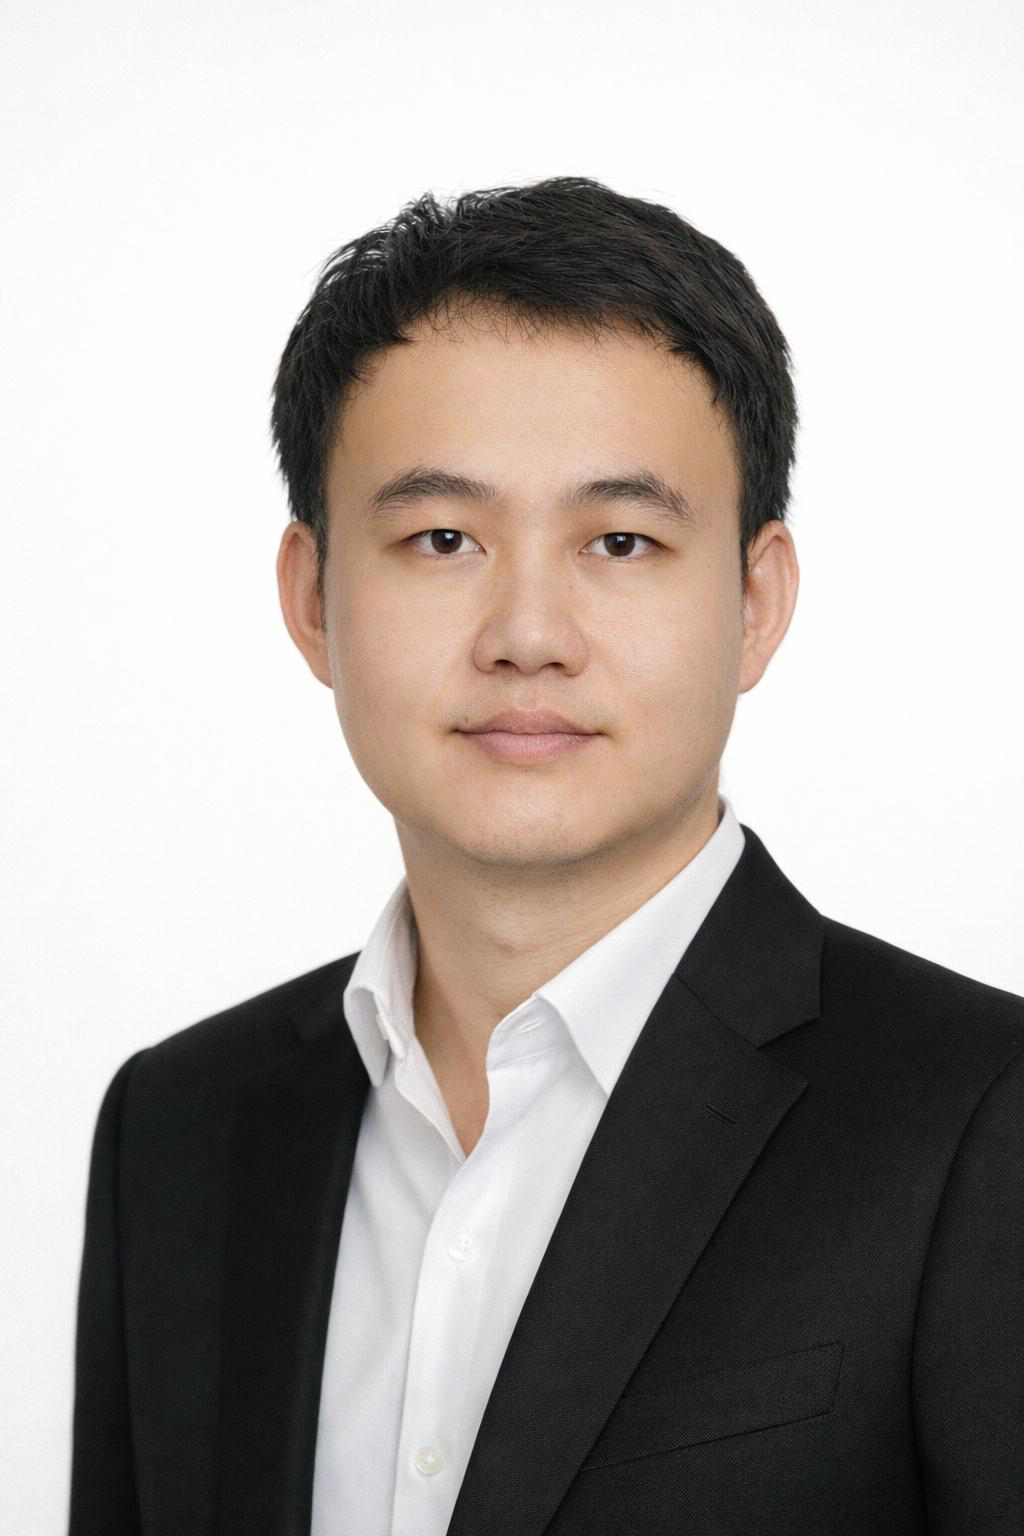
\includegraphics[width=\linewidth]{cv_portrait.png}
\end{minipage}

\medskip
\noindent\textbf{Master's thesis}\\
\emph{Investigating the Impact of Point Cloud Upsampling on
3D Object Detection Performance.}
Implemented preprocessing and evaluation workflows for point-cloud
upsampling on ModelNet40 and KITTI. Compared geometric quality with
PointNet++ classification and PointRCNN/CenterPoint detection results,
and examined detection failures through point-cloud visualizations.
Evaluated downstream detector adaptation to PU-GCN inputs while keeping
the upsampling checkpoint fixed.

\medskip
\noindent\textbf{Seminar project}\\
\emph{GAN-based Generative Modeling for Simulation Data.}
Reviewed the use of generative adversarial networks to generate room
impulse responses for far-field speech recognition. Compared this
approach with analytical room simulation through literature review
and analysis of published experimental results. Examined the role of
synthetic acoustic data under different room conditions, and prepared
a technical report and seminar presentation.

\medskip
\noindent\textbf{Team project --- October 2024--March 2025}\\
\emph{Structure-from-Motion Pipeline.}
Contributed to a pipeline for recovering camera motion and sparse
three-dimensional structure from fisheye image sequences using Python
and OpenCV. Worked on camera calibration, image undistortion and feature
matching using SIFT descriptors, FLANN and RANSAC-based geometric
verification. Visualized feature correspondences, camera geometry and
reconstructed point clouds to check the pipeline outputs.

\bigskip
\noindent
October 2018--January 2023\\
B.Sc.\ in Aerospace Engineering\\
Warsaw University of Technology, Warsaw, Poland

\medskip
\noindent\textbf{Bachelor's thesis}\\
\emph{Monte Carlo Simulation of a Flight After Engine Failure
During the Take-off Process.}
Used Monte Carlo simulation to investigate aircraft flight following
an engine failure during take-off.
\endgroup

    \addcontentsline{toc}{chapter}{Curriculum Vitae}

\end{document}
